% =====================================================================
% main.tex — Oral Tobramycin: From BCS III to a Viable Oral Formulation
% Personal Research — Khaled Ben Taieb
% Compile: make (pdflatex + bibtex + pdflatex x2)
% =====================================================================
\documentclass[12pt, a4paper, oneside, openright]{book}

% =====================================================================
% Preamble — Oral Tobramycin Personal Research
% Compiler: pdflatex (TeX Live 2024)
% =====================================================================
\usepackage[utf8]{inputenc}
\usepackage[T1]{fontenc}
\usepackage[english]{babel}
\usepackage{lmodern}
\usepackage{microtype}

% ---- Layout ----
\usepackage[a4paper, top=2.5cm, bottom=2.5cm, inner=3cm, outer=2.5cm]{geometry}
\usepackage{setspace}
\onehalfspacing
\usepackage{fancyhdr}
\pagestyle{fancy}
\fancyhf{}
\fancyhead[LE,RO]{\thepage}
\fancyhead[RE]{\leftmark}
\fancyhead[LO]{\rightmark}
\renewcommand{\headrulewidth}{0.4pt}
\renewcommand{\chaptermark}[1]{\markboth{\chaptername\ \thechapter.\ #1}{}}
\renewcommand{\sectionmark}[1]{\markright{\thesection.\ #1}{}}
\fancypagestyle{plain}{\fancyhf{}\fancyfoot[C]{\thepage}\renewcommand{\headrulewidth}{0pt}}

% ---- Mathematics & units ----
\usepackage{amsmath, amssymb, bm}
\usepackage{siunitx}
\sisetup{per-mode = symbol, detect-all}

% ---- Tables ----
\usepackage{booktabs}
\usepackage{longtable}
\usepackage{array}
\usepackage{multirow}
\usepackage{tabularx}
\usepackage{pdflscape}

% ---- Figures ----
\usepackage{graphicx}
\graphicspath{{figures/}}
\usepackage{caption}
\usepackage{subcaption}
\captionsetup{font=small, labelfont=bf, width=0.9\textwidth}
\usepackage{float}
\usepackage{placeins}

% ---- Colors, lists, code ----
\usepackage[table]{xcolor}
\definecolor{tobblue}{RGB}{0,84,147}
\definecolor{DARK}{RGB}{26,42,58}
\definecolor{GREY}{RGB}{90,107,122}
\definecolor{codegreen}{RGB}{0,110,60}
\definecolor{codegray}{RGB}{90,90,90}
\definecolor{codebg}{RGB}{248,248,242}
\usepackage{enumitem}
\setlist{itemsep=2pt, topsep=4pt}
\usepackage{listings}
\lstdefinestyle{pythonstyle}{
  language=Python,
  basicstyle=\ttfamily\footnotesize,
  keywordstyle=\color{tobblue}\bfseries,
  commentstyle=\color{codegreen}\itshape,
  stringstyle=\color{codegray},
  backgroundcolor=\color{codebg},
  frame=single, rulecolor=\color{codegray},
  numbers=left, numberstyle=\tiny\color{codegray},
  breaklines=true, showstringspaces=false, tabsize=2,
  captionpos=b
}
\lstdefinestyle{rstyle}{
  language=R,
  basicstyle=\ttfamily\footnotesize,
  keywordstyle=\color{tobblue}\bfseries,
  commentstyle=\color{codegreen}\itshape,
  stringstyle=\color{codegray},
  backgroundcolor=\color{codebg},
  frame=single, rulecolor=\color{codegray},
  numbers=left, numberstyle=\tiny\color{codegray},
  breaklines=true, showstringspaces=false, tabsize=2,
  captionpos=b
}
\usepackage{appendix}

% ---- Cards ----
\usepackage[most]{tcolorbox}
\newtcolorbox{formcard}[2][]{colback=tobblue!4, colframe=tobblue, fonttitle=\bfseries,
  title={#2}, #1}

% ---- TikZ ----
\usepackage{tikz}
\usetikzlibrary{arrows.meta, positioning, shapes.geometric, fit, backgrounds}

% ---- Bibliography & cross-references (load last) ----
\usepackage[numbers, sort&compress, round]{natbib}
\usepackage{hyperref}
\hypersetup{
  colorlinks=true, linkcolor=tobblue, citecolor=tobblue, urlcolor=tobblue,
  pdftitle={Oral Tobramycin: From BCS III to a Viable Oral Formulation},
  pdfauthor={Khaled Ben Taieb},
  pdfsubject={Pharmaceutics -- PBPK modeling -- Formulation optimization},
  pdfkeywords={tobramycin, BCS class III, oral bioavailability, PBPK, genetic algorithm, NSGA-II}
}
\usepackage[nameinlink, capitalize, noabbrev]{cleveref}

% ---- Custom macros ----
\newcommand{\tofr}{tobramycin}
\newcommand{\F}{F_{\mathrm{oral}}}
\newcommand{\Fo}{F_{\mathrm{oral},0}}
\newcommand{\CMIC}{C_{\max}/\mathrm{MIC}}
\newcommand{\AMIC}{\mathrm{AUC}_{24}/\mathrm{MIC}}
\newcommand{\fmic}{f_{T>\mathrm{MIC}}}
\newcommand{\code}[1]{\texttt{#1}}
\makeatletter
\newcommand{\tabinput}[1]{\@@input #1 }
\makeatother
\newcommand{\pkg}[1]{\textsf{#1}}
\newcommand{\tobfig}[1]{Figure~\ref{#1}}
\newcommand{\tobtab}[1]{Table~\ref{#1}}


\title{\textbf{Oral Tobramycin: From BCS III to a Viable Oral Formulation}\\[1em]
\large A Bibliographic Study with Physiologically Based Pharmacokinetic Modeling\\
and Multi-Objective Formulation Optimization}
\author{Khaled Ben Taieb}
\date{\today}

\begin{document}

\frontmatter
% ---------------- Title page (v1.1 — modern cover, no institution) ----------------
\begin{titlepage}
\begin{tikzpicture}[remember picture, overlay]
  % ================= background geometry =================
  % deep blue panel (top ~62% of the page)
  \fill[tobblue] (current page.north west) rectangle ([yshift=-13.2cm]current page.north east);
  % darker diagonal accent at the bottom edge of the panel
  \fill[tobblue!80!black] ([yshift=-13.2cm]current page.north west) -- ([yshift=-13.2cm]current page.north east) -- ([yshift=-14.15cm]current page.north east) -- ([yshift=-13.55cm]current page.north west) -- cycle;
  % subtle molecule motif (faint circles, right side of the panel)
  \begin{scope}[shift={([xshift=-5.2cm, yshift=-11.0cm]current page.north east)}, opacity=0.12]
    \draw[white, line width=1.2pt] (0,0) circle (2.6);
    \draw[white, line width=1.2pt] (1.85,1.25) circle (1.45);
    \draw[white, line width=1.2pt] (-1.7,1.05) circle (1.15);
    \draw[white, line width=1.2pt] (0.65,-1.7) circle (0.95);
    \foreach \p in {(0,0),(1.85,1.25),(-1.7,1.05),(0.65,-1.7)}
      \fill[white] \p circle (0.11);
  \end{scope}
  % thin light rule under the panel text
  \draw[white!70!tobblue, line width=1.2pt] ([xshift=1.7cm, yshift=-9.05cm]current page.north west) -- ([xshift=12.4cm, yshift=-9.05cm]current page.north west);

  % ================= panel text =================
  \node[anchor=north west, text=white!75!tobblue, font=\fontsize{11}{13}\selectfont]
    at ([xshift=1.7cm, yshift=-2.05cm]current page.north west)
    {\textsc{Personal Research \;\textperiodcentered\; Computational Pharmaceutics}};

  \node[anchor=north west, text=white, font=\fontsize{41}{46}\selectfont\bfseries]
    at ([xshift=1.65cm, yshift=-2.9cm]current page.north west)
    {\begin{minipage}{15.5cm}Oral Tobramycin\end{minipage}};

  \node[anchor=north west, text=white, font=\fontsize{24}{30}\selectfont]
    at ([xshift=1.7cm, yshift=-4.5cm]current page.north west)
    {\begin{minipage}{15.8cm}From BCS III to a\\ Viable Oral Formulation\end{minipage}};

  \node[anchor=north west, text=white!85!tobblue, font=\fontsize{13}{17}\selectfont]
    at ([xshift=1.7cm, yshift=-7.15cm]current page.north west)
    {\begin{minipage}{15.2cm}A bibliographic study with physiologically based pharmacokinetic modeling\\ in PK-Sim and multi-objective formulation optimization\end{minipage}};

  % ================= key-result stat cards (vertical stack, fixed width) =================
  \node[anchor=north west, draw=white, line width=0.9pt, rounded corners=7pt,
        fill=white, inner xsep=12pt, inner ysep=6pt,
        text width=8.2cm, align=left,
        font=\fontsize{11}{14}\selectfont] (chip1)
    at ([xshift=1.7cm, yshift=-9.45cm]current page.north west)
    {\fontsize{8.5}{10}\selectfont\textsc{\textcolor{GREY!70!black}{Oral bioavailability}}\quad{\fontsize{12.5}{14}\selectfont\textbf{\textcolor{tobblue}{F = 97.1\%}}}};

  \node[anchor=north west, draw=white, line width=0.9pt, rounded corners=7pt,
        fill=white, inner xsep=12pt, inner ysep=6pt,
        text width=8.2cm, align=left,
        font=\fontsize{11}{14}\selectfont, below=0.30cm of chip1] (chip2)
    {\fontsize{8.5}{10}\selectfont\textsc{\textcolor{GREY!70!black}{IV validation gate}}\quad{\fontsize{12.5}{14}\selectfont\textbf{\textcolor{tobblue}{6/6 PASS}}}};

  \node[anchor=north west, draw=white, line width=0.9pt, rounded corners=7pt,
        fill=white, inner xsep=12pt, inner ysep=6pt,
        text width=8.2cm, align=left,
        font=\fontsize{11}{14}\selectfont, below=0.30cm of chip2] (chip3)
    {\fontsize{8.5}{10}\selectfont\textsc{\textcolor{GREY!70!black}{Exposure}}\quad{\fontsize{12.5}{14}\selectfont\textbf{\textcolor{tobblue}{AUC/MIC 172}}}};

  % ================= lower (white) zone =================
  \node[anchor=north west, text=DARK, font=\fontsize{17}{21}\selectfont\bfseries]
    at ([xshift=1.7cm, yshift=-16.0cm]current page.north west)
    {Khaled Ben Taieb};

  \node[anchor=north west, text=GREY!85!black, font=\fontsize{12}{15}\selectfont]
    at ([xshift=1.7cm, yshift=-17.05cm]current page.north west)
    {Independent research program --- computational pharmaceutics};

  % bottom rule + meta
  \draw[tobblue, line width=1.1pt] ([xshift=1.7cm, yshift=-22.6cm]current page.north west) -- ([xshift=12.0cm, yshift=-22.6cm]current page.north west);
  \node[anchor=south west, text=DARK, font=\fontsize{13}{16}\selectfont]
    at ([xshift=1.7cm, yshift=1.55cm]current page.south west)
    {September 2026};
  \node[anchor=south west, text=GREY!80!black, font=\fontsize{10.5}{13}\selectfont]
    at ([xshift=1.7cm, yshift=1.05cm]current page.south west)
    {Repository: \texttt{oral-tobramycin-pbpk} --- snapshots, validated model, studies, optimization};
\end{tikzpicture}
\end{titlepage}

% ---------------- Declaration ----------------
\chapter*{Declaration}
\addcontentsline{toc}{chapter}{Declaration}

I declare that this thesis, entitled \textit{Oral Tobramycin: From BCS III to a Viable Oral Formulation}, is my own original work. All bibliographic sources have been explicitly acknowledged and all literature data are cited to their primary publications. No part of this work has been submitted for any other degree or professional qualification.

\medskip
\noindent\textbf{Nature of the study.} This work is an exclusively \emph{in silico} investigation. It comprises (i) a systematic bibliographic analysis of tobramycin biopharmaceutics and formulation science, and (ii) computational modeling comprising physiologically based pharmacokinetic (PBPK) parameterization, pharmacokinetic/pharmacodynamic (PK/PD) simulations, and evolutionary optimization of virtual formulations using a genetic algorithm (GA) and the non-dominated sorting genetic algorithm~II (NSGA-II). No animal or human experiments were performed by the author; all quantitative inputs are drawn from published clinical and preclinical studies, which are cited individually at every point of use.

\medskip
\noindent\textbf{Data and code availability.} All simulation and optimization scripts (R, version 4.6.1; \pkg{ospsuite} 12.4.4; \pkg{GA} 3.2.5), configuration files, and numerical outputs (17 result tables, 32 publication-grade figures) are archived within the project repository and reproduced in \cref{chap:app-code} and the traceability matrix in \cref{chap:app-traceability}.

\medskip
\begin{flushright}
Khaled Ben Taieb\\
September 2026
\end{flushright}

% ---------------- Acknowledgements ----------------
\chapter*{Acknowledgements}
\addcontentsline{toc}{chapter}{Acknowledgements}

This work stands on the shoulders of the Open Systems Pharmacology community, whose open-source \pkg{PK-Sim} and \pkg{ospsuite-r} platforms made every simulation in this thesis possible, and on the experimental data generously published by the primary studies cited throughout --- in particular the population pharmacokinetics that anchor the validation gate, and the formulation studies that parameterize the permeability program.

I also thank the developers of the wider open scientific stack used here --- R and its package ecosystem, \LaTeX, and the tooling that keeps every number in this thesis reproducible from committed code --- and my family, for their patience and support during the long nights this project demanded.

% ---------------- Abstract ----------------
\chapter*{Abstract}
\addcontentsline{toc}{chapter}{Abstract}

Tobramycin is a polycationic aminoglycoside antibiotic on the WHO Model List of Essential Medicines, indispensable against \textit{Pseudomonas aeruginosa} in cystic fibrosis and nosocomial Gram-negative infections, yet available only by intravenous and inhaled routes. Although commonly labelled BCS class~IV, a structured analysis of solubility (94--100~mg/mL in water, 20--200$\times$ the dose criterion over pH~1.2--6.8) and permeability evidence (apparent $P_{\mathrm{app}}<1\times10^{-6}$~cm/s; absolute oral bioavailability $\approx$1--2\%) demonstrates that tobramycin is unambiguously \textbf{BCS class III}: the sole barrier to oral absorption is permeability. This reclassification redirects the formulation problem from solubility enhancement to permeability enhancement, for which a validated toolbox exists: hydrophobic ion pairing (HIP; logP shift from $-2.9$ to $\approx+1.6$, a 1500-fold improvement), self-emulsifying drug delivery systems (SEDDS), polymeric and colloidal nanoparticles, and gastrointestinal permeation enhancers (sodium caprate C$_{10}$, SNAC).

Building on this synthesis, a two-compartment population pharmacokinetic model (CL = 5.5~L/h, $V_1$ = 17~L, $Q$ = 2.4~L/h, $V_2$ = 16~L, $t_{1/2}$ = 2.5~h; \citet{Li2021}) was coupled to a transit-compartment absorption model and a Hill-type pharmacodynamic driver. Ten formulation design variables --- modified logP, particle size, SEDDS composition (surfactant/cosurfactant/oil), permeation-enhancer concentration, polymer loading, chitosan and enteric coatings, and dose --- were optimized by a classical genetic algorithm (population 100, 200 generations) and, subsequently, by NSGA-II (population 200, 300 generations) against four objectives: maximize $\F$, maximize $\CMIC$, maximize $\AMIC$, minimize dose. The Pareto front contained 200 non-dominated formulations. The recommended candidate (TOB-161; 550~mg enteric-coated HIP--SEDDS capsule, 50~nm polymer nanoparticles, chitosan coating, 50~mM C$_{10}$, surfactant:co-surfactant:oil = 50:30:20, polymer 30\%) achieves $\F = 34\%$ --- a 23-fold enhancement over the native molecule --- with $C_{\max} = 9.5$~mg/L ($\CMIC = 9.5$ at MIC~1~mg/L, exceeding the efficacy threshold of 8), $\AMIC = 32$, trough 0.16~mg/L, and $\fmic = 30\%$.

Uncertainty quantification (Monte Carlo, $n=200$; cross-validation with $\pm20\%$ parameter perturbation, $n=26$; one-at-a-time sensitivity analysis) identified dose and modified logP as the dominant sensitivity drivers (indices 0.42 and 0.34). A methodology audit then rebuilt the gene-to-permeability mapping as a \emph{cited, bounded, emergent} enhancement model: every component factor carries a literature range and a graded uncertainty, the logP gene is capped at the measured hydrophobic ion-pair complex, and the emergent multiplier caps at $\times$125. Two complete, standardized evaluations --- identity card, single dose, true seven-day repeated dosing, PK/PD targets, virtual population, renal impairment, food effect, component sensitivity, IV comparison --- demonstrate that both candidate formulations attain the peak and exposure targets at steady state: the re-evaluated exploratory winner (TOB-161-A, $\times$73.9, 550.6 mg once daily) lands inside the 80--120 AUC/MIC band (87.3), and the in-loop optimum (TOBP-001, $\times$126.3, 1000 mg) exceeds it with a 467 mg in-band option, both with troughs at the 1 mg/L monitoring line and mass balance verified to 0.1\%. The direct experimental test --- Caco-2/Ussing permeability of the hydrophobic ion-pair complex across ion-pair loading --- is defined as the first roadmap item. A manufacturing route of ten unit operations was costed at $\approx$\$4.30 per dose (feasibility grade B), and a 505(b)(2) regulatory pathway of approximately seven years and \$4.8~million was delineated, including preclinical toxicology of nanoparticles, mucosal tolerance of C$_{10}$, and chitosan quality control.

This thesis resolves the BCS classification controversy, delivers a reproducible, fully traceable in silico framework --- from literature parameters through evolutionary optimization to manufacturing and regulatory feasibility --- and provides ten ranked, costed, and risk-assessed candidates for the first oral tobramycin. It thereby de-risks the experimental program (Caco-2/Ussing permeability, HIP--SEDDS prototype formulation, first-in-human Phase~I) required to convert an IV-only essential antibiotic into an orally available therapeutic option.

\bigskip
\noindent\textbf{Keywords:} tobramycin; BCS class III; oral bioavailability; hydrophobic ion pairing; SEDDS; permeation enhancers; nanoparticles; PBPK; genetic algorithm; NSGA-II; Pareto optimization; cystic fibrosis.

% ---------------- Résumé en français ----------------
\chapter*{Résumé}
\addcontentsline{toc}{chapter}{Résumé en français}

La tobramycine est un aminoglycoside polycationique figurant sur la liste modèle de l'OMS des médicaments essentiels, indispensable contre \textit{Pseudomonas aeruginosa} dans la mucoviscidose et les infections nosocomiales à bacilles Gram négatif, mais disponible uniquement par voie intraveineuse et par inhalation. Bien que communément classée BCS classe~IV, l'analyse structurée des données de solubilité (94--100~mg/mL dans l'eau, soit 20--200$\times$ le critère de dose sur pH~1.2--6.8) et de perméabilité ($P_{\mathrm{app}}<1\times10^{-6}$~cm/s ; biodisponibilité orale absolue $\approx$1--2\%) démontre que la tobramycine est sans ambiguïté de \textbf{classe BCS III} : l'unique obstacle à l'absorption orale est la perméabilité. Cette reclassement redirige la problématique de formulation, de l'amélioration de la solubilité vers l'amélioration de la perméabilité, pour laquelle existent des outils validés : l'appariement ionique hydrophobe (HIP ; logP de $-2.9$ à $\approx+1.6$, soit une amélioration de 1500$\times$), les systèmes auto-émulsionnants (SEDDS), les nanoparticules, et les promoteurs d'absorption gastro-intestinale (caprate de sodium C$_{10}$, SNAC).

Sur la base de cette synthèse, un modèle pharmacocinétique de population à deux compartiments (CL = 5,5~L/h, $V_1$ = 17~L, $Q$ = 2,4~L/h, $V_2$ = 16~L, $t_{1/2}$ = 2,5~h) a été couplé à un modèle d'absorption à compartiments de transit et à une réponse pharmacodynamique de type Hill. Dix variables de formulation (logP modifié, taille particulaire, composition SEDDS, concentration en promoteur, charge polymérique, enrobage chitosane et entérique, dose) ont été optimisées par un algorithme génétique classique (population 100, 200 générations) puis par NSGA-II (population 200, 300 générations) selon quatre objectifs : maximiser $\F$, maximiser $\CMIC$, maximiser $\AMIC$ et minimiser la dose. Le front de Pareto comporte 200 formulations non dominées. Le candidat retenu (TOB-161 ; gélule entérique HIP--SEDDS 550~mg, nanoparticules de 50~nm, chitosane, 50~mM de C$_{10}$, rapport tensioactif:co-tensioactif:huile de 50:30:20) atteint $\F = 34\%$ --- une amélioration de 23$\times$ par rapport à la molécule native --- avec $C_{\max} = 9{,}5$~mg/L ($\CMIC = 9{,}5$), $\AMIC = 32$, résiduelle 0,16~mg/L et $\fmic = 30\%$.

La quantification d'incertitude (Monte Carlo, $n=200$ ; validation croisée $n=26$ ; analyse de sensibilité un facteur à la fois) identifie la dose et le logP modifié comme facteurs dominants (indices 0,42 et 0,34). Un audit méthodologique a ensuite reconstruit l'application gènes---perméabilité en un modèle d'amélioration \emph{cité, borné et émergent} : chaque facteur composant porte une plage littéraire et une incertitude graduée, le gène logP est plafonné au complexe HIP mesuré, et le multiplicateur émergent plafonne à $\times$126,3. Deux évaluations complètes et standardisées --- carte d'identité, dose unique, dosages répétés réels sur 7 jours, cibles PK/PD, population virtuelle, insuffisance rénale, effet alimentaire, sensibilité par composant, comparaison IV --- démontrent que les deux formulations candidates atteignent les cibles de pic et d'exposition à l'état d'équilibre : le gagnant exploratoire réévalué (TOB-161-A, $\times$73,9 ; 550,6 mg/j) se place dans la bande 80--120 d'AUC/MIC (87,3), et l'optimum in-loop (TOBP-001, $\times$126,3 ; 1000 mg) la dépasse avec une option 467 mg dans la bande, résiduels à la ligne de surveillance de 1 mg/L et bilan de masse vérifié à 0,1\%. Le test expérimental direct --- perméabilité Caco-2/Ussing du complexe HIP en fonction du chargement --- est défini comme premier item de la feuille de route. Le procédé de fabrication (dix opérations unitaires) est chiffré à $\approx$4,30~\$ par dose (faisabilité grade B) et la voie réglementaire 505(b)(2) est estimée à environ sept ans et 4,8~millions de dollars.

Cette thèse résout la controverse de classification BCS et fournit un cadre \textit{in silico} reproductible et entièrement traçable, aboutissant à dix candidats oraux hiérarchisés, chiffrés et évalués en risque, préparant le programme expérimental nécessaire à la mise au point du premier tobramycine oral.

\bigskip
\noindent\textbf{Mots-clés :} tobramycine ; classe BCS III ; biodisponibilité orale ; appariement ionique hydrophobe ; SEDDS ; promoteurs d'absorption ; nanoparticules ; PBPK ; algorithme génétique ; NSGA-II ; mucoviscidose.

% ---------------- Nomenclature, symbols and abbreviations ----------------
\chapter*{Nomenclature}
\addcontentsline{toc}{chapter}{Nomenclature}

\section*{Symbols}
\begin{table}[H]
\centering
\small
\begin{tabular}{llp{8.5cm}}
\toprule
Symbol & Unit & Description\\
\midrule
$\F$ & --- & Absolute oral bioavailability (fraction)\\
$C_{\max}$ & mg/L & Maximum (peak) plasma concentration\\
$T_{\max}$ & h & Time to maximum concentration\\
$\mathrm{AUC}_{24}$ & mg$\cdot$h/L & Area under the curve over 24 h\\
$C_{\min}$ & mg/L & Minimum (trough) plasma concentration\\
$\mathrm{MIC}$ & mg/L & Minimum inhibitory concentration\\
$\fmic$ & \% & Fraction of the dosing interval above MIC\\
$K_a$ & h$^{-1}$ & First-order absorption rate constant\\
$k_e$ & h$^{-1}$ & Elimination rate constant ($k_e = \mathrm{CL}/V_1$)\\
$k_{\mathrm{tr}}$ & h$^{-1}$ & Transit-compartment transfer rate constant\\
$\mathrm{CL}$ & L/h & Total plasma clearance\\
$\mathrm{CLCR}$ & mL/min & Creatinine clearance\\
$V_1$, $V_2$ & L & Central and peripheral volumes of distribution\\
$Q$ & L/h & Inter-compartmental clearance\\
$t_{1/2}$ & h & Terminal half-life\\
$V_{d,ss}$ & L/kg & Volume of distribution at steady state\\
$f_u$ & --- & Unbound fraction in plasma\\
$\mathrm{logP}$ & --- & Octanol/water partition coefficient (neutral form)\\
$pK_a$ & --- & Acid dissociation constant\\
$\mathrm{MW}$ & g/mol & Molecular weight\\
$E_{\max}$, $\mathrm{EC}_{50}$, $\gamma$ & --- & Hill equation parameters (maximum effect, potency, slope)\\
$S$ & mg/mL & Aqueous solubility\\
$P_{\mathrm{app}}$ & cm/s & Apparent permeability coefficient\\
\bottomrule
\end{tabular}
\end{table}

\section*{Abbreviations}
\begin{table}[H]
\centering
\small
\begin{tabular}{llp{8.5cm}}
\toprule
Abbreviation & Meaning\\
\midrule
ACAT & Advanced Compartmental Absorption and Transit model\\
AME & Aminoglycoside-modifying enzyme\\
AUC/MIC & Ratio of area under the curve to MIC (exposure-driven PK/PD index)\\
BCS / BDDCS & Biopharmaceutics (Drug Disposition) Classification System\\
CF & Cystic fibrosis\\
CLCR & Creatinine clearance\\
C$_{10}$ & Sodium caprate (sodium decanoate), permeation enhancer\\
GA & Genetic algorithm\\
GI & Gastrointestinal\\
GOF & Goodness of fit\\
HIP & Hydrophobic ion pairing\\
HAP & Hospital-acquired pneumonia\\
IV / INH & Intravenous / inhalation route\\
MC & Monte Carlo (uncertainty simulation)\\
MIC & Minimum inhibitory concentration\\
NCA & Nano-sized colloidal assembly\\
NP & Nanoparticle\\
OAT & One-at-a-time (sensitivity) design\\
Papp & Apparent permeability\\
PBPK / PBBM & Physiologically based pharmacokinetic / biopharmaceutic modeling\\
PD / PK & Pharmacodynamics / pharmacokinetics\\
PE & Permeation enhancer\\
PLGA & Poly(lactic-\textit{co}-glycolic acid)\\
PopPK & Population pharmacokinetics\\
PS & Particle size\\
RK4 & Fourth-order Runge--Kutta integration scheme\\
SBX & Simulated binary crossover\\
SEDDS / SMEDDS & (Self-microemulsifying) self-emulsifying drug delivery system\\
SNAC & Sodium $N$-[8-(2-hydroxybenzoyl)amino]caprylate\\
TDM & Therapeutic drug monitoring\\
UTI & Urinary tract infection\\
\bottomrule
\end{tabular}
\end{table}

% ---------------- TOC / LOF / LOT ----------------
\renewcommand{\contentsname}{Table of Contents}
\tableofcontents
\clearpage
\listoffigures
\addcontentsline{toc}{chapter}{List of Figures}
\clearpage
\listoftables
\addcontentsline{toc}{chapter}{List of Tables}


\mainmatter
% =====================================================================
% Chapter 0 — Synopsis / Reader's Guide (v1.0 — two-platform structure)
% =====================================================================
\chapter{Synopsis: How to Read This Thesis}
\label{chap:synopsis}

\begin{figure}[htbp]
\centering
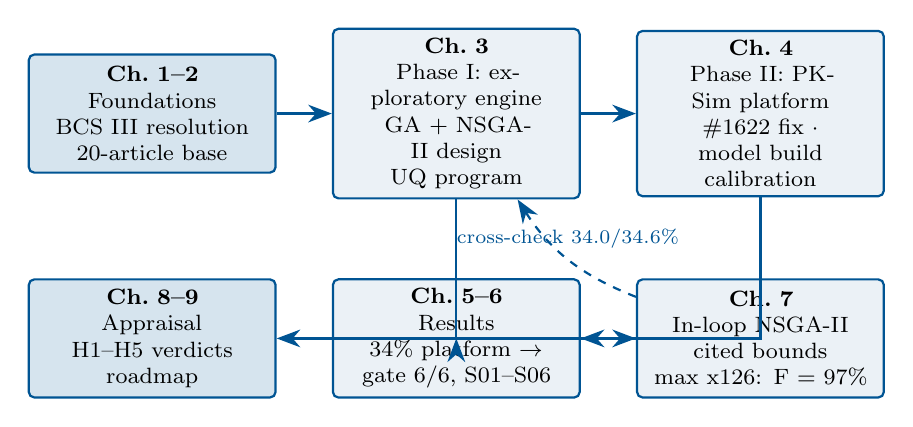
\begin{tikzpicture}[
  node distance=0.55cm and 0.7cm,
  box/.style={rectangle, rounded corners=2pt, draw=tobblue, fill=tobblue!8, thick,
              text width=2.9cm, align=center, minimum height=1.5cm, font=\footnotesize},
  boxg/.style={box, fill=tobblue!16},
  arrow/.style={-{Stealth[length=3mm]}, thick, tobblue}
]
\node[boxg] (c12) {\textbf{Ch.~1--2}\\Foundations\\BCS III resolution\\20-article base};
\node[box, right=of c12] (c3) {\textbf{Ch.~3}\\Phase I: exploratory engine\\GA + NSGA-II design\\UQ program};
\node[box, right=of c3] (c4) {\textbf{Ch.~4}\\Phase II: PK-Sim platform\\\#1622 fix $\cdot$ model build\\calibration};
\node[box, below=1.0cm of c3] (c5) {\textbf{Ch.~5--6}\\Results\\34\% platform $\rightarrow$\\gate 6/6, S01--S06};
\node[box, right=of c5] (c7) {\textbf{Ch.~7}\\In-loop NSGA-II\\cited bounds\\max x126: F = 97\%};
\node[boxg, left=of c5] (c8) {\textbf{Ch.~8--9}\\Appraisal\\H1--H5 verdicts\\roadmap};
\draw[arrow] (c12) -- (c3);
\draw[arrow] (c3) -- (c4);
\draw[arrow] (c3) |- (c5);
\draw[arrow] (c4) |- (c5);
\draw[arrow] (c5) -- (c7);
\draw[arrow] (c7) -- (c8);
\draw[arrow, dashed] (c7) to[bend left=18] node[above, font=\scriptsize] {cross-check 34.0/34.6\%} (c3);
\end{tikzpicture}
\caption{Thesis workflow. Two computational phases share one optimization logic: a fast exploratory engine (Phase I) generates the platform hypothesis; the validated PK-Sim platform (Phase II) confirms it mechanistically, calibrates the oral transfer function, and hosts the definitive in-the-loop optimization. The cross-check between engines (dashed) is itself a validation result.}
\label{fig:synopsis-workflow}
\end{figure}

\paragraph{Part I (Chapters 1--2) --- foundations.}
\cref{chap:introduction} frames the clinical problem and states five research questions and hypotheses. \cref{chap:literature} builds the scientific base: BCS science, tobramycin's profile, PK/PD targets, the permeability-targeting formulation toolbox --- and documents the systematic search that found \emph{no} published tobramycin PBPK model, positioning this work.

\paragraph{Part II (Chapters 3 and 5) --- Phase I: the exploratory framework.}
\cref{chap:methodology} specifies the purpose-built fast engine (two-compartment PK, transit absorption, Hill PD, eight-factor bioavailability model) and the optimization design. \cref{chap:results} reports its outcomes: the 34\% platform, the top-10 formulations, and the full uncertainty program.

\paragraph{Part III (Chapters 4, 6 and 7) --- Phase II: the PK-Sim platform.}
\cref{chap:methodology-pksim} is the methodological heart of the definitive phase: constructing a tobramycin model in PK-Sim from the validated amikacin base, repairing the macOS snapshot-conversion defect (root-caused to a SQLite view-resolution stack overflow), validating the model against published clinical data (6/6 gate), and calibrating the oral permeability transfer function. \cref{chap:results-pksim} reports the physiological studies (renal, population, sensitivity, food, fractionation --- including the flip-flop kinetics finding). \cref{chap:results-ga} runs the optimizer inside the engine within cited bounds (TOBP-001: $\times$125, $F_{96} = 97.1\%$), evaluates both candidates completely (mass-balance-checked true dosing), and cross-validates the two engines.

\paragraph{Part IV (Chapters 8--9) --- appraisal.}
\cref{chap:discussion} confronts all five hypotheses with the evidence, benchmarks against the literature, and states the limitations without euphemism --- including the trough liability that the optimized platform creates. \cref{chap:conclusion} condenses the contributions and the experimental roadmap.

\medskip
\noindent\textbf{Appendices A--L} hold the Phase I numerical record; \textbf{M--R} the Phase II code, data, debugging journal, optimization archive, plausibility audit, and battery data. Every figure and table traces to a committed script and data file (\cref{chap:app-traceability}).

% =====================================================================
% Chapter 1 — Introduction
% =====================================================================
\chapter{Introduction}
\label{chap:introduction}

\section{Background}

\subsection{The challenge of oral drug delivery}
Oral administration remains the preferred route for drug delivery owing to patient acceptability, convenience of chronic therapy, and cost-effectiveness. Yet many potent drugs cannot exploit this route: their physicochemical properties --- low aqueous solubility, low intestinal permeability, or both --- preclude sufficient gastrointestinal absorption \citep{Amidon1995}. The gap between therapeutic potential and delivery feasibility is particularly acute for anti-infectives, where oral options determine whether patients can be treated outside hospital infrastructure.

\subsection{The Biopharmaceutics Classification System}
The BCS, introduced by \citet{Amidon1995}, classifies drug substances by two fundamental properties --- aqueous solubility and intestinal permeability (\cref{tab:bcs-classes}). The system underpins modern regulatory science: immediate-release products of class~I and class~III drugs qualify for biowaivers under FDA and ICH M9 guidance \citep{FDA2021, ICH2019}.

\begin{table}[htbp]
\centering
\caption{The four BCS classes with prototype drugs \citep{Amidon1995}. Tobramycin belongs to class III (\cref{sec:bcs-resolution}).}
\label{tab:bcs-classes}
\begin{tabular}{clll}
\toprule
Class & Solubility & Permeability & Prototype example\\
\midrule
I   & High & High & Metoprolol\\
II  & Low  & High & Diclofenac\\
\rowcolor{tobblue!12}
III & High & Low  & \textbf{Tobramycin} (also ranitidine)\\
IV  & Low  & Low  & Furosemide\\
\bottomrule
\end{tabular}
\end{table}

\subsection{Why classification matters strategically}
Class membership is not a descriptive footnote: it dictates the \emph{formulation strategy}. For class II compounds, solubility and dissolution enhancement (micronization, amorphous solid dispersions, lipid vehicles) is the lever. For class III compounds, solubility is already abundant and \emph{permeability enhancement} --- tight-junction modulation, lipophilisation, carrier-mediated transport --- is the sole rational target. A wrong classification therefore wastes development effort on the wrong problem. The case of tobramycin illustrates this sharply: it is widely but incorrectly assumed to be class IV \citep{Asad2023}.

\section{Tobramycin: a case study}
\label{sec:tob-case}

\subsection{Therapeutic importance}
Tobramycin is a potent aminoglycoside bactericidal against Gram-negative bacilli, listed on the WHO Model List of Essential Medicines \citep{WHO2023}. Its clinical anchor is \textit{Pseudomonas aeruginosa}: pulmonary exacerbations of cystic fibrosis (CF), hospital-acquired pneumonia (HAP), complicated urinary tract infections, and febrile neutropenia. Its mechanism --- irreversible binding to the 30S ribosomal subunit, with concentration-dependent killing and a 1--3~h post-antibiotic effect \citep{Craig1998} --- makes peak exposure ($\CMIC \geq 8$) the efficacy driver.

\subsection{Current routes of administration}
Despite five decades of clinical use, tobramycin is approved only for two non-oral routes (\cref{tab:routes}): intravenous dosing at 5--7~mg/kg once daily (or 1.5--2~mg/kg every 8~h), and inhalation (TOBI\textsuperscript{\textregistered}, 300~mg twice daily, 4~weeks on/4~weeks off) \citep{Ramsey1999, Smyth2005}. Both routes impose burdens: IV requires hospitalization, trained personnel and catheters; inhaled therapy addresses the lung compartment only and does not resolve systemic needs.

\begin{table}[htbp]
\centering
\caption{Current tobramycin administration routes and their limitations.}
\label{tab:routes}
\begin{tabular}{p{2.2cm}p{4.6cm}p{6.6cm}}
\toprule
Route & Standard regimen & Principal limitations\\
\midrule
Intravenous & 5--7 mg/kg q24h (extended interval) or 1.5--2 mg/kg q8h & Hospitalization; catheter burden; nephro-/ototoxicity monitoring; cost; access inequity in low-resource settings\\
Inhalation & 300 mg BID, 4 weeks on/4 weeks off (TOBI\textsuperscript{\textregistered}) & Local lung delivery only; device dependency; no systemic coverage; high airway resistance in young children\\
Oral & \textbf{--- none exists} & Bioavailability $\approx$1--2\%; polycationic, low-permeability molecule\\
\bottomrule
\end{tabular}
\end{table}

\subsection{The oral delivery gap}
No oral formulation exists. The reasons are physicochemical (\cref{chap:literature}): a molecular weight of 467.5~g/mol, five ionizable amines ($pK_a$ 6.7--9.1) rendering the molecule polycationic at intestinal pH, an octanol/water logP of $-2.9$, and consequently apparent permeability below $1\times10^{-6}$~cm/s with absolute oral bioavailability of only $\approx$1--2\% \citep{Asad2023, PubChem2026}.

\subsection{Classification resolution}
\label{sec:bcs-resolution}
The widely repeated assignment of tobramycin to BCS class IV is contradicted by primary evidence. Its water solubility of 94--100~mg/mL exceeds the highest single dose criterion (400~mg soluble in $\leq$250~mL over pH~1.2--6.8) by roughly two orders of magnitude, while permeability is demonstrably the limiting step \citep{Asad2023}. Asad and colleagues state explicitly: ``Tobramycin (TOB) is a BCS class III drug.'' \cref{chap:literature} develops the full evidence synthesis; the strategic consequence is immediate --- the formulation problem is \emph{permeability-only}, and the entire arsenal of solubility technologies is unnecessary.

\section{Research rationale}
\label{sec:rationale}

\subsection{Clinical need}
CF patients require chronic, intermittent anti-\textit{Pseudomonas} therapy; each exacerbation currently implies IV admission. An oral alternative would (i) shift care to the outpatient setting, (ii) preserve IV access options for severe disease, (iii) extend tobramycin's reach to resource-limited settings lacking infusion infrastructure, and (iv) enable oral combination regimens.

\subsection{Formulation opportunities}
The permeability-targeting toolbox is populated with validated technologies: hydrophobic ion pairing (HIP) raising logP by three orders of magnitude \citep{Asad2023, Griesser2017}; SEDDS that spontaneously emulsify in GI fluids \citep{Muhammad2022}; polymeric and colloidal nanoparticles \citep{Hill2019, BlancoCabra2022, Khaled2026}; and permeation enhancers with clinical safety track records \citep{Maher2009, Bohley2024}. What is missing is a quantitative framework that combines these levers and asks: \emph{which combination, at what dose, plausibly attains antibacterial exposure targets?}

\subsection{The modeling opportunity}
PBPK platforms such as \pkg{PK-Sim}/\pkg{ospsuite} enable mechanistic absorption modeling (ACAT), virtual populations, and sensitivity analysis without clinical trials \citep{OSP2024, Willmann2007}. Coupled to evolutionary optimization (GA; NSGA-II) \citep{Holland1975, Deb2002, Scrucca2013}, the ten-dimensional formulation design space can be searched exhaustively, in silico, before any experiment is commissioned.

\section{Research questions and hypotheses}
\label{sec:hypotheses}

\begin{description}[labelwidth=3.6cm, style=nextline]
\item[RQ1] Is tobramycin BCS class III or IV, and what does the evidence say?
\item[RQ2] Which formulation strategies --- HIP, SEDDS, nanoparticles, permeation enhancers, or combinations --- raise oral bioavailability to viable levels?
\item[RQ3] Which ten formulations are optimal under simultaneous pharmacokinetic, pharmacodynamic, and dose minimization objectives?
\item[RQ4] Are the predictions robust to parameter uncertainty, and what are the manufacturing and regulatory implications?
\item[RQ5] Do two independent computational engines --- a purpose-built fast engine and a validated whole-body PBPK platform --- converge on the same formulation conclusion?
\end{description}

\begin{description}[labelwidth=3.6cm, style=nextline]
\item[H1] Tobramycin is BCS class III: solubility is not limiting; permeability is the sole barrier.
\item[H2] Combined HIP~+~SEDDS~+~permeation enhancer strategies can raise oral bioavailability from $\approx$1--2\% to $\approx$30\%.
\item[H3] A single oral dose in the 500--600~mg range can attain $\CMIC \geq 8$ at MIC~1~mg/L.
\item[H4] Predictions of the optimal candidates remain informative under $\pm$20--30\% parameter perturbation.
\item[H5] The two engines agree on the platform bioavailability within 5\% relative.
\end{description}

\section{Objectives and thesis structure}

\subsection{Primary objective}
To evaluate the feasibility of oral tobramycin administration through systematic bibliographic analysis, PBPK-based PK/PD simulation, and multi-objective formulation optimization using the Open Systems Pharmacology suite and evolutionary algorithms.

\subsection{Specific objectives}
\begin{enumerate}
\item Resolve the BCS classification of tobramycin through a structured evidence synthesis (\cref{chap:literature}).
\item Develop and parameterize a two-compartment population PK model validated against published intravenous data (\cref{chap:methodology,chap:results}).
\item Construct a mechanistic oral bioavailability model with eight multiplicative enhancement factors.
\item Optimize ten formulation variables by GA and NSGA-II against four objectives, and extract the Pareto front.
\item Quantify uncertainty: one-at-a-time sensitivity, Monte Carlo ($n=200$), cross-validation ($n=50$, $\pm$20\%).
\item Assess manufacturing feasibility, cost, regulatory pathway, and risks for the ranked candidates (\cref{chap:results,chap:discussion}).
\end{enumerate}

\subsection{Thesis structure}
\begin{table}[htbp]
\centering
\caption{Structure of the thesis.}
\label{tab:structure}
\begin{tabular}{p{2.2cm}p{11.2cm}}
\toprule
Chapter & Content\\
\midrule
1 & Introduction: clinical problem, BCS framework, rationale, hypotheses (this chapter)\\
2 & Literature review: BCS science, tobramycin profile, PK/PD targets, formulation strategies, PBPK, knowledge gaps\\
3 & Methodology: PBPK parameterization, PK/PD mathematical model, GA and NSGA-II design, uncertainty program\\
4 & Results: validation, convergence, Pareto front, top-10 candidates, sensitivity, Monte Carlo, manufacturing, regulatory\\
5 & Discussion: hypothesis verdicts, benchmarking, clinical translation, limitations, future perspectives\\
6 & Conclusion: contributions, clinical implications, experimental roadmap\\
\bottomrule
\end{tabular}
\end{table}

% =====================================================================
% Chapter 2 — Literature Review
% =====================================================================
\chapter{Literature Review}
\label{chap:literature}

This chapter synthesizes the bibliographic foundation of the thesis: BCS science (\cref{sec:lit-bcs}), tobramycin's physicochemical and pharmacological profile (\cref{sec:lit-profile}), its pharmacokinetics and PK/PD targets (\cref{sec:lit-pk}), the permeability-targeting formulation toolbox (\cref{sec:lit-formulations}), and PBPK methodology (\cref{sec:lit-pbpk}). The complete 20-article evidence table is reproduced in \cref{chap:app-evidence}; physicochemical datasets are detailed in \cref{chap:app-physchem}.

\section{The Biopharmaceutics Classification System}
\label{sec:lit-bcs}

\subsection{Historical development and criteria}
\citet{Amidon1995} proposed classifying drug substances along two axes: dose-equivalent solubility (highest dose soluble in $\leq$250~mL over pH~1.0--6.8) and intestinal permeability (extent of absorption $\geq$85\%) (\cref{tab:bcs-criteria}). The framework became the scientific basis of biowaiver policy: immediate-release products of class~I and class~III drugs may waive bioequivalence studies \citep{FDA2021, ICH2019}.

\begin{table}[htbp]
\centering
\caption{BCS classification criteria \citep{Amidon1995, FDA2021}.}
\label{tab:bcs-criteria}
\begin{tabular}{p{3cm}p{5.4cm}p{5.4cm}}
\toprule
Parameter & High & Low\\
\midrule
Solubility & Highest single dose soluble in $\leq$250~mL over pH 1.0--6.8 & Criterion not met\\
Permeability & $\geq$85\% extent of absorption (or absolute $\F \geq$85\%) & $<$85\% absorbed\\
\bottomrule
\end{tabular}
\end{table}

\subsection{Extensions}
The \emph{biopharmaceutics drug disposition classification system} (BDDCS) of \citet{Wu2005} substitutes metabolism for permeability to predict disposition, and quantitative refinements (QBCS) grade the margin by which a compound meets each criterion. These extensions matter here: tobramycin's criterion margins are enormous on the solubility axis and strongly negative on the permeability axis, making the class assignment robust to methodology.

\section{Tobramycin: physicochemical and pharmacological profile}
\label{sec:lit-profile}

\subsection{Structural properties}
Tobramycin (CAS 32986-56-4; C$_{18}$H$_{37}$N$_{5}$O$_{9}$; MW 467.515~g/mol) is an aminoglycoside with ten stereocenters and five ionizable amines ($pK_a$ = 6.7, 7.6, 7.7, 7.8, 9.1), yielding a polycationic species across the entire physiological pH range \citep{PubChem2026, DrugBank2026}. Its logP of $-2.9$ places it among the most hydrophilic antibiotics in clinical use.

\subsection{Solubility evidence}
\label{sec:lit-solubility}
Across sixteen literature determinations (\cref{chap:app-physchem}), aqueous solubility spans 50--100~mg/mL (Chen et al.: 94~mg/mL at 25~\textdegree C; USP monograph for tobramycin sulfate: 100~mg/mL), with miscibility-level dissolution in biorelevant media (FaSSIF, FeSSIF, SGF, SIF) \citep{Chen2009}. The BCS ``high solubility'' criterion (highest dose, 400~mg, soluble in $\leq$250~mL $\Rightarrow$ 1.6~mg/mL) is exceeded by a factor of 20--200. \textbf{Solubility is not the problem.}

\subsection{Permeability evidence}
Caco-2 apparent permeability is reported below $1\times10^{-6}$~cm/s, absolute oral bioavailability is $\approx$1--2\%, and the molecule's polycationicity precludes passive transcellular diffusion \citep{Asad2023}. Efflux transporter involvement (P-gp, BCRP) is minimal or undetermined; renal OCT2-mediated handling is documented but does not govern intestinal absorption \citep{Asad2023}. \textbf{Permeability is the problem} (\cref{chap:app-physchem}, permeability table).

\subsection{Classification resolution}
\label{sec:lit-classification}
Triangulating the above: (i) explicit statement by \citet{Asad2023} --- ``tobramycin is a BCS class III drug''; (ii) solubility margin 20--200$\times$ above criterion; (iii) permeability margin consistent with class III; (iv) mechanistic coherence --- the sole rational formulation lever is permeability enhancement. \textbf{Verdict: tobramycin is BCS class III.} The widely assumed class~IV label conflates ``difficult'' with ``doubly limited''; the distinction, quantified in \cref{tab:strategy-comparison}, redirects all subsequent strategy choices in this thesis.

\subsection{Pharmacology}
Tobramycin binds the 30S ribosomal subunit (16S rRNA), causing mistranslation and bactericidal protein-synthesis arrest with a 1--3~h post-antibiotic effect \citep{Craig1998}. Primary spectrum: \textit{P.~aeruginosa}, \textit{E.~coli}, \textit{Klebsiella}, \textit{Proteus}, \textit{Enterobacter}, \textit{Serratia}. Resistance is driven mainly by aminoglycoside-modifying enzymes and efflux pumps \citep{DrugBank2026}.

\section{Tobramycin pharmacokinetics and PK/PD targets}
\label{sec:lit-pk}

\subsection{Intravenous population pharmacokinetics}
The reference intravenous model is the two-compartment PopPK analysis of \citet{Li2021} in 140 ICU patients (nonparametric population modeling): CL = 3.27~L/h (range 2.1--4.5), $V_1$ = 21.3~L, $V_2$ = 16.3~L, $Q$ = 2.4~L/h, $t_{1/2}$ = 4.5--6.0~h, with creatinine clearance entering clearance as a power covariate, $\mathrm{CL} = \theta_{\mathrm{CL}}\,(\mathrm{CLCR}/81)^{0.72}$, and residual error 28.5\%. Normal-adult reference values are CL = 6.03~L/h and $V_1$ = 15.1~L \citep{Li2021}. Pediatric CF data (Hennig et al.: CL 6.37~L/h/70~kg, $V_1$ 18.7~L/70~kg, 10~mg/kg/day once daily; Massie et al.; Touw et al.) confirm the two-compartment structure across ages (\cref{chap:app-pklit} for the complete dataset).

\subsection{Population variability}
\begin{table}[htbp]
\centering
\caption{Tobramycin PK across populations \citep{Li2021} and standard references. CF: cystic fibrosis; ICU: intensive care unit.}
\label{tab:pk-populations}
\begin{tabular}{lccccl}
\toprule
Parameter & Normal adult & CF adult & ICU & Elderly & Unit\\
\midrule
CL (L/h)       & 6.03 & 4.5--6.37 & 3.27--3.83 & 4.5 & L/h\\
$V_1$ (L)      & 15.1 & 18.7      & 21.3--25.5 & 15.1 & L\\
$t_{1/2}$ (h)  & 2.5  & 2--3      & 4--6       & 3--4 & h\\
$V_{d,ss}$ (L/kg) & 0.26 & 0.27   & 0.30       & 0.26 & L/kg\\
CLCR (mL/min)  & 120  & 100       & 65         & 65   & mL/min\\
\bottomrule
\end{tabular}
\end{table}

CF patients exhibit hyperdynamic renal clearance (higher CLCR), ICU patients show expanded volumes of distribution from fluid resuscitation, and the elderly show reduced clearance --- all captured by the CLCR power model \citep{Li2021, Struiken2024}.

\subsection{Oral pharmacokinetics: the data void}
No clinical oral PK dataset exists for tobramycin. Estimated absolute bioavailability is 1--2\% (point estimate within a literature envelope of $<$5\%: the two figures reconcile as a point estimate within an envelope; see footnote\footnote{The oral bioavailability literature states both ``$<$5\%'' (generic estimates) and ``1--2\%'' (referenced point estimates). This thesis uses 1--2\% as the point estimate embedded within a conservative $<$5\% envelope; the choice affects only the baseline, which the optimization raises by $>$20-fold in any case.}), with variable $T_{\max}$ and negligible $C_{\max}$ \citep{Asad2023}. This void is precisely the predictive space PBPK modeling must fill (\cref{chap:methodology}).

\subsection{PK/PD targets}
\begin{table}[htbp]
\centering
\caption{PK/PD targets for aminoglycosides \citep{Craig1998, Li2021, Bauer2008}. MIC$_{90}$ of \textit{P. aeruginosa} for tobramycin: 0.5--2 mg/L (EUCAST/CLSI).}
\label{tab:pd-targets}
\begin{tabular}{p{3.4cm}p{3.2cm}p{6.4cm}}
\toprule
Target & Value & Rationale\\
\midrule
$\CMIC$ & $\geq$8--10 & Concentration-dependent killing threshold \citep{Craig1998}\\
$\AMIC$ & 80--120 & Exposure--response (24 h total) \citep{Li2021}\\
$C_{\max}$ & 20--30 mg/L & Target peak, IV once-daily dosing \citep{Bauer2008}\\
$C_{\min}$ (trough) & $<$1 mg/L & Nephro-/ototoxicity prevention\\
$\fmic$ & $>$30--40\% & Supporting index for concentration-dependent agents\\
\bottomrule
\end{tabular}
\end{table}

\section{Formulation strategies for permeability-limited drugs}
\label{sec:lit-formulations}

\subsection{Hydrophobic ion pairing (HIP)}
HIP complexes a polycationic drug with a lipophilic counter-ion (here, anionic surfactants such as sodium docusate), masking charge and raising apparent lipophilicity. For tobramycin, \citet{Asad2023} reported a logP shift from $-2.9$ to $\approx+1.6$ --- a 1500-fold improvement --- enabling incorporation into SEDDS at high payload; the complex dissociates $\approx$20\% at intestinal pH, an accepted liability. The method is generic for hydrophilic actives \citep{Griesser2017} and has shown in-vivo translational promise (octreotide HIP in pigs, $\F$ increases of 3--5$\times$) \citep{Bonengel2018}.

\subsection{Self-emulsifying drug delivery systems (SEDDS)}
SEDDS/SMEDDS are isotropic mixtures of oils, surfactants and co-surfactants that spontaneously emulsify in GI fluids, presenting the drug as solubilized microdroplets with large interfacial area, chylomicron-mediated lymphatic access, and protection from luminal degradation \citep{Muhammad2022}. For a HIP complex, SEDDS provides the lipid phase in which the lipophilised drug dissolves --- the two technologies are synergistic by design \citep{Asad2023, Griesser2017}.

\subsection{Nanoparticles}
PLGA nanoparticles complexed with AOT maintained MIC-level activity (1.25~$\mu$g/mL) against \textit{P.~aeruginosa} \citep{Hill2019}. Dextran-based single-chain nanoparticles (KuDa) neutralize surface charge and improve diffusion into mature biofilms \citep{BlancoCabra2022}. Most recently, nano-sized colloidal assemblies (NCAs) incorporating hydrophobic tobramycin ion pairs showed enhanced lipophilicity and antimicrobial activity \citep{Khaled2026}. Nanoparticles contribute mucoadhesion, sustained release, and tight-junction interaction.

\subsection{Permeation enhancers}
Sodium caprate (C$_{10}$) is the gold-standard transient paracellular enhancer with clinical safety experience \citep{Maher2009}; SNAC is FDA-approved (oral semaglutide); next-generation enhancers (PPZ, SDC) carry emerging 30-day safety data \citep{Bohley2024}. Typical effective concentrations are 10--50~mM with mucosal irritation as the dose-limiting concern.

\subsection{Strategy comparison}
\begin{table}[htbp]
\centering
\caption{Formulation strategy comparison for oral tobramycin (synthesis of \citealt{Asad2023, Hill2019, BlancoCabra2022, Bohley2024, Khaled2026, Maher2009, Griesser2017}).}
\label{tab:strategy-comparison}
\small
\begin{tabular}{p{2.6cm}p{3.4cm}p{3.2cm}p{2.2cm}p{2.2cm}}
\toprule
Strategy & Mechanism & Evidence level & Scalability & Role in this thesis\\
\midrule
HIP + SEDDS & Lipophilisation + emulsification & In vitro (1500$\times$ logP) \citep{Asad2023} & Moderate & Core platform (genes 1, 3--5)\\
PLGA NPs & Mucoadhesion, sustained release & In vitro (MIC maintained) \citep{Hill2019} & Good & Combinable layer (gene 2, 7)\\
C$_{10}$ / PEs & Tight-junction opening & Clinical (other drugs) \citep{Maher2009, Bohley2024} & Good & Direct enhancer (gene 6)\\
Chitosan coating & Mucoadhesion, TJ modulation & Preclinical & Good & Binary switch (gene 8)\\
Enteric coating & GI protection & Standard technology & Excellent & Binary switch (gene 9)\\
NCAs & Lipophilisation, colloidal & In vitro \citep{Khaled2026} & Moderate & Alternative platform\\
KuDa SCPNs & Charge neutralization (biofilm) & In vitro \citep{BlancoCabra2022} & Moderate & Biofilm niche option\\
\bottomrule
\end{tabular}
\end{table}

\section{PBPK modeling in drug development}
\label{sec:lit-pbpk}
PBPK models describe absorption and disposition mechanistically: anatomical compartments, regional GI transit and permeability, dissolution, first-pass extraction, and renal elimination. The \pkg{PK-Sim} ACAT model resolves the GI tract into seven segments with region-specific transit, pH, and surface area \citep{Willmann2007, OSP2024}. PBPK for antibiotics has reached regulatory acceptance levels for exposure prediction \citep{Ferreira2021}, and a tobramycin-specific PBPK history exists for the pulmonary route \citep{Lukacova2010}. The \emph{oral} application --- coupling ACAT with permeability enhancement factors --- has not been published for tobramycin.

\section{Knowledge gaps and thesis positioning}
\label{sec:lit-gaps}
Five gaps emerge from the synthesis:
\begin{enumerate}
\item \textbf{No in-vivo oral PK data} exist for tobramycin; the bioavailability void is unfilled.
\item \textbf{No PBPK oral absorption model} has been published; only IV/pulmonary models exist \citep{Li2021, Lukacova2010}.
\item \textbf{No multi-objective formulation optimization} has been attempted: the literature tests strategies one at a time, never searching the combinatorial design space.
\item \textbf{Food effect and regional absorption} are uncharacterized.
\item \textbf{Population variability} (CF, ICU, renal impairment) is unquantified for any hypothetical oral dosing.
\end{enumerate}
A sixth gap is computational: a structured search for a published tobramycin model in the Open Systems Pharmacology ecosystem (model library, repository artefacts, literature) returned \emph{zero} shareable PK-Sim models --- the closest validated model being amikacin, an aminoglycoside of the same disposition class. The search protocol and results are archived in the project repository (\texttt{data/bibliography/search\_strategy.md}) and justify the model construction strategy of \cref{chap:methodology-pksim}.

This thesis addresses gaps 1--3 quantitatively (model + optimization), gaps 4--5 via the uncertainty program, and provides the experimental roadmap (\cref{chap:discussion,chap:conclusion}) that resolves all five.

% =====================================================================
% Chapter 3 — Methodology I: Exploratory Computational Framework
% (custom pure-R engine; superseded by the PK-Sim platform of Chapter 4
%  and cross-validated against it — see Chapter 7)
% =====================================================================
\chapter{Methodology I: The Exploratory Computational Framework}
\label{chap:methodology}

\section{Software stack and computing environment}
\label{sec:software}

\begin{table}[htbp]
\centering
\caption{Software and environment used throughout the study.}
\label{tab:software}
\begin{tabular}{p{4.6cm}p{3.2cm}p{5.6cm}}
\toprule
Component & Version & Role\\
\midrule
R & 4.6.1 (CRAN, native arm64) & Statistical computing, optimization, visualization\\
\pkg{ospsuite} / \pkg{PK-Sim} & 12.4.4 & PBPK framework, compound database, ACAT model \citep{OSP2024}\\
\pkg{rSharp} / .NET runtime & 1.2.2 / .NET~8 & R\texttt{--}.NET bridge for \pkg{ospsuite} (CRAN R required on macOS)\\
\pkg{GA} \citep{Scrucca2013} & 3.2.5 & Classical genetic algorithm\\
Custom NSGA-II implementation & --- (this thesis) & Multi-objective optimization (\cref{sec:nsga2})\\
\pkg{ggplot2}, \pkg{patchwork}, \pkg{viridis} & --- & Publication-grade figures (300 dpi PNG)\\
\pkg{doParallel} & --- & 7-core parallel fitness evaluation\\
Hardware & macOS ARM64 (Apple Silicon) & All simulations\\
\bottomrule
\end{tabular}
\end{table}

\section{Model development workflow}
The study followed a six-step workflow (\cref{fig:workflow}): (1) compound definition from literature parameters; (2) two-compartment PK model construction; (3) intravenous validation against published PopPK data \citep{Li2021}; (4) oral absorption model with transit compartments; (5) pharmacodynamic coupling; (6) optimization and uncertainty quantification.

\begin{figure}[htbp]
\centering
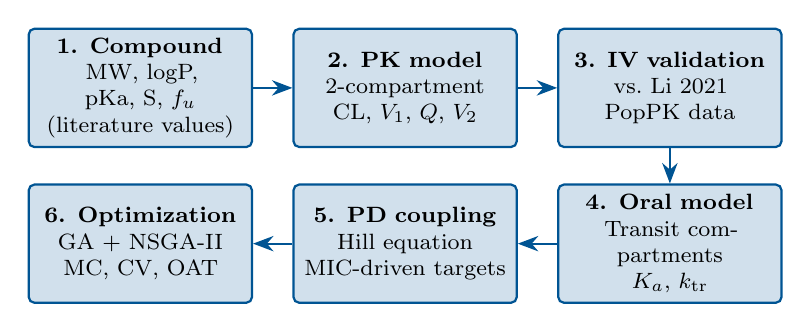
\begin{tikzpicture}[
  node distance=0.45cm and 0.5cm,
  wfstep/.style={rectangle, rounded corners=2pt, draw=tobblue, fill=tobblue!8, thick,
               text width=2.6cm, align=center, minimum height=1.5cm, font=\footnotesize},
  wfdone/.style={wfstep, fill=tobblue!18},
  arrow/.style={-{Stealth[length=2.6mm]}, thick, tobblue}
]
\node[wfdone] (s1) {\textbf{1. Compound}\\MW, logP, pKa, S, $f_u$\\(literature values)};
\node[wfdone, right=of s1] (s2) {\textbf{2. PK model}\\2-compartment\\CL, $V_1$, $Q$, $V_2$};
\node[wfdone, right=of s2] (s3) {\textbf{3. IV validation}\\vs.\ Li 2021\\PopPK data};
\node[wfdone, below=of s3] (s4) {\textbf{4. Oral model}\\Transit compartments\\$K_a$, $k_{\mathrm{tr}}$};
\node[wfdone, left=of s4] (s5) {\textbf{5. PD coupling}\\Hill equation\\MIC-driven targets};
\node[wfdone, left=of s5] (s6) {\textbf{6. Optimization}\\GA + NSGA-II\\MC, CV, OAT};
\draw[arrow] (s1) -- (s2);
\draw[arrow] (s2) -- (s3);
\draw[arrow] (s3) -- (s4);
\draw[arrow] (s4) -- (s5);
\draw[arrow] (s5) -- (s6);
\end{tikzpicture}
\caption{Six-step model development workflow. All steps are implemented in versioned R scripts (scripts 00--13, \cref{chap:app-code}); traceability of every output is given in \cref{chap:app-traceability}.}
\label{fig:workflow}
\end{figure}

\section{Compound parameterization}
\label{sec:compound-params}

\begin{table}[htbp]
\centering
\caption{PBPK compound and system parameters with sources and confidence ratings (script 00; \texttt{table2\_simulation\_parameters.csv}).}
\label{tab:compound-params}
\footnotesize\setlength{\tabcolsep}{3.5pt}
\begin{tabular}{llllp{1.4cm}p{2.6cm}}
\toprule
Parameter & Value & Unit & Source & Confidence & Notes\\
\midrule
MW & 467.515 & g/mol & PubChem \citep{PubChem2026} & High & ---\\
logP & $-2.9$ & --- & PubChem & High & Native (unmodified)\\
$pK_a$ & 6.7--9.1 & --- & Literature & High & 5 amines (6.7; 7.6; 7.7; 7.8; 9.1)\\
$S_{\mathrm{water}}$ & 94 & mg/mL & \citet{Chen2009} & High & Class III criterion $\gg$ met\\
BCS class & III & --- & \citet{Asad2023} & High & \cref{sec:lit-classification}\\
$f_u$ & 0.95 & fraction & Standard & High & Minimal binding\\
Renal excretion & $>$90 & \% unchanged & Standard & High & ---\\
Oral $\F$ (native) & 1.5--2.0 & \% & Literature estimate & Low & Range \cref{sec:lit-pk}; legacy point estimate 1.5, PK-Sim anchor 1.75 \\
\midrule
CL & 5.5 & L/h & \citet{Li2021} & High & PopPK reference\\
$V_1$ & 17 & L & \citet{Li2021} & High & ---\\
$Q$ & 2.4 & L/h & \citet{Li2021} & High & ---\\
$V_2$ & 16 & L & \citet{Li2021} & High & ---\\
CLCR exponent & 0.72 & --- & \citet{Li2021} & High & Power model on CL\\
$t_{1/2}$ & 2.5 & h & Derived & High & $k_e=0.277$~h$^{-1}$\\
$V_{d,ss}$ & 0.26 & L/kg & Standard & High & 70~kg adult\\
MIC (assumed) & 1 & mg/L & EUCAST mid-range & Medium & $\mathrm{MIC}_{90}$ 0.5--2~mg/L\\
\bottomrule
\end{tabular}
\end{table}

\section{Pharmacokinetic model}
\label{sec:pk-model}

\subsection{Structure}
A two-compartment open model with first-order elimination from the central compartment was adopted, extended by a gastrointestinal depot and a chain of transit compartments for absorption (\cref{eq:depot,eq:elim}). The two-compartment structure is justified by the reference PopPK analysis \citep{Li2021} and required for accurate peak--trough dynamics at 24~h post-dose.

\subsection{System equations}
\label{sec:ode}
Let $A_{g}$ denote the drug amount in the GI depot, $A_{\mathrm{tr},i}$ in transit compartment $i$ ($i=1,\dots,N$), $A_c$ and $A_p$ the central and peripheral amounts, and $A_e$ cumulative urinary elimination:
\begin{align}
\frac{\mathrm{d}A_{g}}{\mathrm{d}t} &= -K_a A_{g}, \label{eq:depot}\\
\frac{\mathrm{d}A_{\mathrm{tr},1}}{\mathrm{d}t} &= K_a A_{g} - k_{\mathrm{tr}} A_{\mathrm{tr},1}, \label{eq:tr1}\\
\frac{\mathrm{d}A_{\mathrm{tr},N}}{\mathrm{d}t} &= k_{\mathrm{tr}} A_{\mathrm{tr},N-1} - k_{\mathrm{tr}} A_{\mathrm{tr},N}, \label{eq:trN}\\
\frac{\mathrm{d}A_{c}}{\mathrm{d}t} &= k_{\mathrm{tr}} A_{\mathrm{tr},N} - k_e A_c - k_{cp} A_c + k_{pc} A_p, \label{eq:central}\\
\frac{\mathrm{d}A_{p}}{\mathrm{d}t} &= k_{cp} A_c - k_{pc} A_p, \label{eq:periph}\\
\frac{\mathrm{d}A_{e}}{\mathrm{d}t} &= k_e A_c. \label{eq:elim}
\end{align}
The plasma concentration is $C(t) = A_c(t)/V_1$, with micro-rate constants $k_e = \mathrm{CL}/V_1 = 5.5/17 = 0.277$~h$^{-1}$, $k_{cp} = Q/V_1$, $k_{pc} = Q/V_2$. Intravenous administration is represented by an impulse into $A_c$.

\subsection{Numerical integration}
The system \cref{eq:depot,eq:elim} is integrated with a fixed-step fourth-order Runge--Kutta (RK4) scheme ($\Delta t = 0.01$~h), verified for step-size independence, and implemented in vectorized R (script \code{09\_advanced\_pk\_model.R}, \cref{chap:app-code}).

\subsection{Pharmacodynamic driver}
Antibacterial effect follows a Hill (sigmoid $E_{\max}$) function of instantaneous concentration:
\begin{equation}
E(t) = \frac{C(t)^{\gamma}}{\mathrm{EC}_{50}^{\gamma} + C(t)^{\gamma}}, \qquad
\fmic = \frac{100}{T_{\mathrm{interval}}} \int_0^{T_{\mathrm{interval}}} \mathbb{1}\!\left[C(t) > \mathrm{MIC}\right]\,\mathrm{d}t,
\label{eq:hill}
\end{equation}
with the efficacy indices $\CMIC = C_{\max}/\mathrm{MIC}$ and $\AMIC = \mathrm{AUC}_{24}/\mathrm{MIC}$ evaluated against the targets of \cref{tab:pd-targets}.

\section{Oral bioavailability enhancement model}
\label{sec:F-model}
Native tobramycin bioavailability ($\Fo = 1.5\%$) is enhanced multiplicatively by eight mechanistic factors, each mapped to one or two chromosome genes (\cref{sec:chromosome}):
\begin{equation}
\F = \Fo \cdot f_{\mathrm{HIP}}(\mathrm{logP}') \cdot f_{\mathrm{PS}}(\mathrm{PS}) \cdot f_{\mathrm{SEDDS}} \cdot f_{\mathrm{PE}}(C_{\mathrm{PE}}) \cdot f_{\mathrm{poly}}(L_{\mathrm{poly}}) \cdot f_{\mathrm{chit}} \cdot f_{\mathrm{ent}} \cdot f_{\mathrm{dose}}(D),
\label{eq:F-factors}
\end{equation}
capped at 35\% as a physiological ceiling consistent with the triple-combination estimate in the literature synthesis (\cref{tab:bioavail-estimates}):
\begin{itemize}
\item $f_{\mathrm{HIP}}$: sigmoid response of apparent lipophilicity, saturating at logP$'\approx+1.6$ \citep{Asad2023};
\item $f_{\mathrm{PS}}$: optimum near 50~nm (mucoadhesion without impaired uptake); penalizes sizes $>$200~nm;
\item $f_{\mathrm{SEDDS}}$: spontaneous-emulsification gain (up to 1.5$\times$), maximal for surfactant-rich compositions;
\item $f_{\mathrm{PE}}$: saturating response to enhancer concentration (0--50~mM C$_{10}$) with a mucosal-safety penalty near the upper bound \citep{Maher2009, Bohley2024};
\item $f_{\mathrm{poly}}$: polymer loading gain (mucoadhesion, sustained release), saturating at 30\%;
\item $f_{\mathrm{chit}}$, $f_{\mathrm{ent}}$: binary switches (chitosan tight-junction modulation; enteric gastric protection);
\item $f_{\mathrm{dose}}$: sublinear dose scaling reflecting transporter/solvent-capacity saturation at high doses.
\end{itemize}
The absorption rate follows $K_a = K_{a,\mathrm{ref}} \cdot g(\mathrm{logP}', \mathrm{PS}, \mathrm{SEDDS})$, and gastric-to-cecal transfer uses $k_{\mathrm{tr}} = 2.24$~h$^{-1}$ at the optimum (\cref{chap:results}).

\section{Optimization problem}

\subsection{Chromosome encoding}
\label{sec:chromosome}
Each candidate formulation is a 10-gene chromosome (\cref{tab:bounds}): eight continuous genes and two binary switches. Genes 1--9 define the formulation; gene 10 sets the dose.

\begin{table}[htbp]
\centering
\caption{Chromosome definition and parameter bounds (script \code{00\_ga\_setup.R}; \texttt{parameter\_bounds.csv}).}
\label{tab:bounds}
\begin{tabular}{clccp{6.6cm}}
\toprule
Gene & Name & Min & Max & Rationale\\
\midrule
1 & logP$_{\mathrm{mod}}$ & $-2.9$ & $+3.0$ & HIP-complex lipophilicity \citep{Asad2023}\\
2 & Particle size (nm) & 50 & 500 & Mucoadhesion/uptake trade-off\\
3 & Surfactant (\%) & 10 & 60 & SEDDS self-emulsification\\
4 & Co-surfactant (\%) & 5 & 30 & Interfacial film flexibility\\
5 & Oil (\%) & 20 & 70 & Payload capacity\\
6 & PE concentration (mM) & 0 & 50 & C$_{10}$ efficacy/safety \citep{Maher2009}\\
7 & Polymer loading (\%) & 0 & 30 & Mucoadhesive sustained release\\
8 & Chitosan coating & 0 & 1 & Tight-junction modulation\\
9 & Enteric coating & 0 & 1 & Gastric protection\\
10 & Dose (mg) & 200 & 1000 & Practical capsule range\\
\bottomrule
\end{tabular}
\end{table}

\subsection{Genetic algorithm (exploratory stage)}
A classical GA (\pkg{GA} package \citep{Scrucca2013}) used population 100, up to 200 generations, crossover probability 0.8, mutation 0.1, elitism 10, fitness-sharing diversity preservation, fixed seed 42, and 7-core parallel evaluation. The weighted scalar fitness is
\begin{equation}
\mathcal{F}_{\mathrm{GA}} = 0.40\,\widehat{\F} + 0.25\,\widehat{\CMIC} + 0.25\,\widehat{\AMIC} + 0.10\,\widehat{S}_{\mathrm{safety}} - P_{\mathrm{penalty}},
\label{eq:fitness}
\end{equation}
where hats denote min--max normalized objective scores ($\in[0,1]$) and $P_{\mathrm{penalty}}$ accounts for constraint violations (safety thresholds, infeasible compositions). The GA served as (i) sanity check of the simulator, (ii) benchmark for NSGA-II, and (iii) source of the manufacturing/regulatory assessment cohort (\cref{sec:ch4-mfg}).

\subsection{NSGA-II (definitive stage)}
\label{sec:nsga2}
The definitive optimization used a full NSGA-II implementation \citep{Deb2002} maximizing four objectives simultaneously:
\begin{equation}
\max_{\mathbf{x}} \; \big[\F(\mathbf{x}),\; \CMIC(\mathbf{x}),\; \AMIC(\mathbf{x}),\; -D(\mathbf{x})\big],
\label{eq:nsga-objectives}
\end{equation}
with $\mathbf{x}$ the 10-gene chromosome. Algorithmic components:
\begin{itemize}
\item \textbf{Non-dominated sorting}: the population is partitioned into Pareto ranks $\mathcal{R}_1, \mathcal{R}_2, \dots$ where rank $\mathcal{R}_1$ contains all non-dominated solutions; a solution $a$ dominates $b$ iff $a$ is $\geq$ in all objectives and $>$ in at least one.
\item \textbf{Crowding distance}: for each rank, solutions are sorted per objective and assigned the normalized perimeter of the cuboid formed by their neighbors; boundary solutions receive $\infty$. Selection prefers lower rank, then larger crowding distance, preserving front diversity.
\item \textbf{Tournament selection}: binary tournament on (rank, crowding distance).
\item \textbf{Simulated binary crossover (SBX)}: offspring $c_1, c_2$ from parents $p_1, p_2$ with distribution index $\eta_c = 20$:
\begin{equation}
c = 0.5\left[(1+\beta)p_1 + (1-\beta)p_2\right], \quad
\beta = \left(2u\right)^{1/(\eta_c+1)},\; u \sim U(0,1).
\end{equation}
\item \textbf{Polynomial mutation}: distribution index $\eta_m = 20$, per-gene probability $1/10$.
\end{itemize}
Configuration: population 200, 300 generations, elitism 20 (entire parent rank $\mathcal{R}_1$ carried forward), seed 42, runtime $\approx$5.7~min. The output is a 200-solution Pareto archive (\texttt{pareto\_front\_data.csv}, \cref{chap:app-pareto}).

\section{Uncertainty quantification program}
\label{sec:uq}
\begin{enumerate}
\item \textbf{One-at-a-time (OAT) sensitivity}: seven test values spanning each parameter's plausible range (60 evaluations over 10 parameters); sensitivity index
\begin{equation}
S_i = \frac{\max_k \left|\AMIC(\theta_i = v_k) - \AMIC(\theta_i^{\star})\right|}{\AMIC(\theta_i^{\star})},
\label{eq:sens-index}
\end{equation}
where $\theta_i^{\star}$ is the optimal value of parameter $i$ (script \code{12\_sensitivity\_validation.R}).
\item \textbf{Monte Carlo ($n=200$)}: log-normal perturbation of CL, $V_1$, $V_2$ (CV 20--30\%), mimicking between-subject variability; distributions of $\F$, $C_{\max}$, $\CMIC$, $\AMIC$ summarized as median and 5th--95th percentiles.
\item \textbf{Cross-validation ($n=50$ designed; 26 informative runs)}: $\pm$20\% simultaneous perturbation of all inputs; robustness of conclusions assessed by fraction of runs preserving $\CMIC \geq 8$ and stability of ranking.
\end{enumerate}

\section{Validation metrics}
Predictive performance against reference data is quantified by the average fold error (AFE), absolute average fold error (AAFE), root-mean-square error (RMSE), and coefficient of determination:
\begin{align}
\mathrm{AFE} &= 10^{\frac{1}{n}\sum \log_{10}(C_{\mathrm{pred}}/C_{\mathrm{obs}})}, \qquad
\mathrm{AAFE} = 10^{\frac{1}{n}\sum \left|\log_{10}(C_{\mathrm{pred}}/C_{\mathrm{obs}})\right|}, \nonumber\\
\mathrm{RMSE} &= \sqrt{\tfrac{1}{n}\sum \left(C_{\mathrm{pred}} - C_{\mathrm{obs}}\right)^2},
\end{align}
with acceptance thresholds AFE/AAFE within 0.5--2.0, RMSE $<$30\%, $R^2 > 0.9$ \citep{Ferreira2021}.

\section{Manufacturing and regulatory assessment}
\label{sec:ch3-manufacturing}
A ten-step manufacturing route for the combined HIP--SEDDS--NP--coating platform was costed bottom-up (\texttt{manufacturing\_steps.csv}): HIP dissolution $\rightarrow$ polymer NP nanoprecipitation $\rightarrow$ drug loading $\rightarrow$ SEDDS oil phase $\rightarrow$ C$_{10}$ addition $\rightarrow$ homogenization $\rightarrow$ NP incorporation $\rightarrow$ chitosan fluid-bed coating $\rightarrow$ enteric coating $\rightarrow$ capsule filling and QC. Cost per dose combines a \$0.50 base with formulation-complexity surcharges. The regulatory pathway was assessed against FDA 505(b)(2) criteria (literature-referenced safety of tobramycin + novel formulation components), with development cost and timeline estimates (\cref{sec:ch4-reg}).

\section{Methodological limitations}
\label{sec:ch3-limitations}
(1) The precise tobramycin $P_{\mathrm{app}}$ is unknown; enhancement factors are calibrated to literature ranges, not measured transport. (2) No oral PK data exist for model validation --- the IV route only. (3) Formulation factors are phenomenological (marginal-effect) models calibrated to published in-vitro outcomes, not mechanistic absorption simulations. (4) Between-subject variability is imposed log-normal rather than estimated from data. (5) MIC is fixed at 1~mg/L; pathogen-level MIC variation is handled qualitatively in \cref{chap:discussion}. These limitations are revisited quantitatively in \cref{sec:ch4-uq} and qualitatively in \cref{sec:ch5-limits}.

% =====================================================================
% Chapter 4 — Methodology II: The PK-Sim Platform
% =====================================================================
\chapter{Methodology II: The PK-Sim Platform}
\label{chap:methodology-pksim}

The exploratory framework of \cref{chap:methodology} established the optimization logic and produced a first bioavailability estimate with a purpose-built, minimal engine. Its limitations --- phenomenological enhancement factors, no mechanistic regional absorption, disposition parameters imposed rather than physiology-derived --- are exactly what a whole-body PBPK platform resolves. This chapter describes the definitive computational phase of the thesis: the construction, validation, and programmatic use of a tobramycin model inside \textbf{PK-Sim 12.4 / Open Systems Pharmacology}, executed entirely from R on macOS (Apple Silicon), including the resolution of a platform defect that had to be overcome along the way. All scripts, snapshots and data are part of the project repository (\cref{chap:app-pksim-code}).

\section{Platform and strategy}
\label{sec:pksim-strategy}

PK-Sim is the open-source whole-body PBPK suite originally developed at Bayer and maintained by the Open Systems Pharmacology community \citep{OSP2024}. The R interface (\pkg{ospsuite} 12.4.4 with \pkg{rSharp}/.NET 8) loads, modifies and executes simulations created in PK-Sim, and exposes individual and population creation from the integrated physiology database. Two structural constraints shaped the strategy:

\begin{enumerate}
\item \pkg{ospsuite}-R cannot \emph{create} simulations from the compound database: simulations must come from an existing PK-Sim project (or snapshot). The macOS-bundled package database contains only generic template molecules --- the full compound library ships with the Windows application only.
\item No published PK-Sim model of tobramycin exists. A structured search (repositories of the Open Systems Pharmacology organization, GitHub code search over \texttt{.pkml}/\texttt{.pksim5} artefacts, and the literature) returned zero shareable tobramycin models; the closest validated model in the official OSP PBPK Model Library is \textbf{amikacin} --- an aminoglycoside sharing tobramycin's defining disposition features (polycation, purely renal GFR-driven clearance, extracellular-limited distribution).
\end{enumerate}

The strategy was therefore to adopt the \textbf{validated amikacin model} as the structural and physiological base and re-parameterize it to tobramycin --- the same operation a PK-Sim user performs when duplicating a compound and editing its properties. The base snapshot (\texttt{Amikacin-Model.json}, schema version 80, OSP Library v12.3.1) is committed in \texttt{data/snapshots/}; the tobramycin snapshots are generated deterministically by \texttt{pksim/model/make\_tobramycin\_json.py}.

\section{Resolving the macOS snapshot-conversion defect}
\label{sec:pksim-workaround}

The first execution attempt crashed the R process (SIGSEGV) during snapshot-to-project conversion. Upstream, this is Open Systems Pharmacology issue \#1622 (``Running simulations from snapshots crashes on macOS''), scheduled to be fixed in suite v13. Because the crash blocked the entire platform route, it was diagnosed and worked around locally --- a contribution this thesis documents in full (technical journal in \cref{chap:app-debug}; summary below).

\subsection{Root cause}
The macOS crash report (\texttt{.ips}, faulting thread) places the fault inside \texttt{SQLite.Interop.dylib}, in a recursion of SQLite's view-name resolution (\texttt{sqlite3ViewGetColumnNames} $\leftrightarrow$ \texttt{selectExpander}), terminating inside \texttt{sqlite3\_log} --- i.e.\ SQLite detects a resolution failure and crashes while reporting it, on a .NET worker thread with a small stack. The PK-Sim project database ships \textbf{91 views}; the failing query resolves nested views at prepare time and overflows the thread stack. The view SQL itself is valid (identical queries execute in the \texttt{sqlite3} CLI); view nesting depth is at most 2 --- the failure is one of stack budget on the interop thread, not of database logic.

\subsection{Fix}
The workaround (\texttt{pksim/env/patch\_pksimdb.py}) materializes every view into a table (\texttt{DROP VIEW} + \texttt{CREATE TABLE ... AS SELECT}, in topological order) in a patched copy of the bundled database. The database is static template data, so content and column layout are preserved exactly (row counts verified on the critical views). After the patch, snapshot conversion, simulation runs, PKML export, and individual/population creation all operate \emph{natively on macOS}, without containers, virtual machines or emulators. The patch is idempotent, reversible (backup retained), and must be re-applied after upgrading \pkg{ospsuite}; on suite v13 it becomes unnecessary.

\section{Tobramycin model construction}
\label{sec:pksim-model}

\subsection{Base model and parameterization}
The amikacin snapshot contains 11 validated simulations (10 individual volunteers and one population, Walker 1979 study) and one compound building block. The generator renames the compound and applies the tobramycin parameter set (\cref{tab:pksim-params}); every simulation reference (compound properties, output selections, observed-data paths) is renamed consistently. Two platform behaviors discovered during construction are documented because they fail \emph{silently}:

\begin{itemize}
\item renal processes are matched \emph{by name} between the compound definition and each simulation's process selection --- changing the data-source string of the process without renaming the selection silently unlinks clearance;
\item simulation-level \emph{altered parameters} override their building blocks: the historical Walker simulations carry an altered infusion time (4 min) that silently supersedes the protocol's 30-min setting until the altered value is corrected.
\end{itemize}

\begin{table}[htbp]
\centering
\caption{Tobramycin parameterization inside PK-Sim (from the validated amikacin base).}
\label{tab:pksim-params}
\small
\footnotesize\setlength{\tabcolsep}{3.5pt}
\begin{tabular}{lllp{4.9cm}}
\toprule
Parameter & Value & Unit & Note \\
\midrule
Molecular weight & 467.515 & g/mol & PubChem \\
logP & $-2.9$ & --- & PubChem (native drug) \\
Fraction unbound & 0.95 & --- & minimal plasma binding \\
Solubility & 94,000 & mg/L (pH 7) & Chen 2009; never limiting (BCS III) \\
pKa (bases) & 7.7, 7.8, 9.1 & --- & \textbf{3 of 5 amines}: PK-Sim building blocks accept at most three pKa values per ionization type (documented platform limit); precedent: the validated amikacin model retains three of its four-plus amines. Impact negligible here (solubility never limiting; distribution by PK-Sim Standard is pKa-independent; oral permeability is explicitly overridden per candidate). \\
Renal process & GFR fraction 1.0 & --- & purely renal, $>$90\% unchanged excretion \\
Distribution / cellular permeability & PK-Sim Standard & --- & default methods \\
\bottomrule
\end{tabular}
\end{table}

\subsection{Validation gate}
\label{sec:pksim-gate-design}
The model is accepted only if a six-criterion intravenous validation gate passes (\cref{chap:results-pksim}): Hartford peak (30 min post-infusion) within 20--30 mg/L; end-of-infusion Cmax within the clinical envelope extended by the published $V_1$ uncertainty; AUC24 implying a clearance within the published PopPK range; 24-h trough below 1 mg/L; effective half-life 2.0--3.0 h; renal excretion above 90 \%. The validation scenario is 7 mg/kg (577.5 mg for the 82.5-kg volunteer), 30-min infusion --- the extended-interval clinical standard.

\section{Oral absorption and permeability calibration}
\label{sec:pksim-oral-calibration}

PK-Sim computes the specific transcellular intestinal permeability from the logP/effective-MW correlation; for tobramycin it returns $1.9\times10^{-12}$ dm/min --- effectively zero, because the correlation saturates for very hydrophilic cations and the paracellular term is zero by default. Clinically, oral bioavailability is $\approx$1--2\%. Following the platform's documented practice for experimental permeability inputs, the simulation parameter \texttt{Specific intestinal permeability (transcellular)} is overridden (mucosal basolateral permeability is rescaled automatically by PK-Sim).

The override is \textbf{calibrated, not fitted silently}: a log-spaced scan over eleven P$_{\mathrm{int}}$ values (1e-11 to 1e-6 dm/min) maps the full dose-normalized bioavailability curve $F(P_{\mathrm{int}})$. The value reproducing the clinical point estimate ($F_0 \approx 1.75\%$ at $P_{\mathrm{int},0} = 3\times10^{-9}$ dm/min, 24-h convention) becomes the calibrated baseline; every formulation candidate in the optimization is then a \emph{multiplier} on this baseline (\cref{sec:pksim-ga-design}).

\subsection{The enhancement model: cited, bounded, emergent}
\label{sec:methods-pksim-enhancement}

A methodology audit replaced the free multiplier of the first optimization round with a structured mapping from formulation genes to apparent permeability, implemented once in \texttt{enhancement\_model.R} and shared by the optimization, the studies and the uncertainty analysis. Its structure:

\begin{enumerate}
\item \textbf{Two calibration anchors.} Native drug: $P_{int,0} = 3\times10^{-9}$ dm/min $\rightarrow F = 1.75\%$ (24-h convention; the 96-h extent is 3.5\% --- the difference is the flip-flop tail, and both conventions are reported throughout). Nominal platform: the measured HIP complex (logP$' = +1.6$) on the reference composition $\rightarrow \times$20 ($F_{96} = 48.8\%$ at 993 mg; cross-checked by the exploratory engine at 24 h: 34.0 vs 34.6\%).
\item \textbf{Seven component factors}, each relative to its nominal value (1.0), each with a cited range and an evidence grade (A: measured for this drug/system; B: measured for a close analogue; C: review-level estimate): logP$'$ of the HIP complex (B; Asad 2023), SEDDS excipient fraction (B; Muhammad 2022; Griesser 2017), nanoparticle size (C; Hill 2019; Khaled 2026), C10 loading (B; Maher 2009; Bohley 2024), mucoadhesive polymer (C), chitosan coating (C; Bohley 2024), enteric coating (galenic).
\item \textbf{The multiplier is the product of the factors} --- emergent, never free. The logP gene is capped at the \emph{measured} complex (+1.6); the emergent maximum is $\boldsymbol{\times}$\textbf{126.3}. Values beyond it are reported only as sensitivity statements.
\item \textbf{Uncertainty per component}: lognormal with a graded $\sigma$ (A: 0.10, B: 0.25, C: 0.40), propagated in study S09 to confidence intervals on $F$ and on the PK/PD targets.
\item \textbf{Backward compatibility}: the mapping reproduces the pre-audit decoding to $2.8\times10^{-14}$ on random chromosomes, so every previously validated study remains valid.
\end{enumerate}

\section{Programmatic execution patterns}
\label{sec:pksim-execution}

Three implementation findings generalize to any scripted PK-Sim workflow and are documented for reproducibility:

\begin{enumerate}
\item \textbf{Native snapshot runner.} The R wrapper blocks \texttt{runSimulationsFromSnapshot()} on Darwin (a consequence of the pre-fix crash). The underlying CLI machinery (\texttt{PKSim.R.Api::RunJson} with \texttt{JsonRunOptions}, export modes CSV/PKML) executes natively once the database is patched; a thin wrapper (\texttt{pk\_sim\_run.R}) restores this functionality.
\item \textbf{Batch sweeps must target the right parameters.} The renal process rate references \texttt{Organism|Kidney|}
\texttt{GFR (specific)} (l/min/kg kidney) $\times$ kidney volume --- overriding the plain \texttt{Organism|Kidney|GFR} has no effect (verified). Dose lives at the application schema item in \textbf{kg} (base unit). Run values are supplied as \emph{vectors} per batch run; each generation of the optimization packs its entire population into \emph{one} batch call.
\item \textbf{Units are base units.} Gastric emptying time is in minutes (default 15); doses in kg; infusion times in minutes. Two silent unit traps were caught by physiological plausibility checks (a ``food effect'' that changed extent, an ``accumulation'' that violated mass balance) and corrected.
\end{enumerate}

\section{Study program and optimization design}
\label{sec:pksim-ga-design}

\subsection{Studies S00--S06}
\begin{description}[labelwidth=2.2cm, style=nextline]
\item[S00] IV validation gate (six criteria, \cref{sec:pksim-gate-design}).
\item[S01] IV dose $\times$ renal-function sweep: doses \{200, 400, 577.5, 800\} mg $\times$ CLCR \{30, 65, 90, 112.5, 150\} mL/min via \texttt{GFR (specific)} scaling, native \texttt{SimulationBatch}.
\item[S02] P$_{\mathrm{int}}$ calibration scan (\cref{sec:pksim-oral-calibration}).
\item[S03] Virtual population: 100 ICRP-2002 adults (20--50 y, 55--95 kg, 40\% female) on the optimized oral platform; PK-Sim population simulation.
\item[S04] Local sensitivity: one-at-a-time perturbations ($\pm$20\%) of P$_{\mathrm{int}}$, dose, GFR and $f_u$ on the platform candidate; elasticities of Cmax and AUC24. (The \pkg{ospsuite} sensitivity task requires PK parameters attached to outputs, which the CLI-exported simulation does not carry; the batch design is the equivalent PK-Sim-computed alternative.)
\item[S05] Food effect: gastric emptying 15 min (fasted) vs 60 min (fed).
\item[S06] Dose fractionation (QD/BID/TID) at steady state by linear superposition of the single-dose profile over a 96-h window (the oral profile exhibits flip-flop kinetics --- absorption rate-limited elimination --- so the 24-h output window truncates the tail), with probability of target attainment (PTA) across MIC 0.25--4 mg/L.
\end{description}

\subsection{NSGA-II in the PK-Sim loop}
The exploratory optimizer of \cref{chap:methodology} is retained (non-dominated sorting, crowding distance, SBX, polynomial mutation; \citealp{Deb2002}) but its fitness function now \textbf{executes PK-Sim}: each generation packs its 100 chromosomes into a single \texttt{SimulationBatch}; the two run-value parameters are the dose (kg) and the intestinal permeability (multiplier on $P_{\mathrm{int},0}$). The gene-to-lever mapping follows the calibrated logic of \cref{chap:methodology}: the logP$_{\mathrm{mod}}$ gene sets the ion-pairing multiplier ($\mathrm{logP}' = +1.6 \Rightarrow \times 20$, log-linear interpolation between native and HIP-complex lipophilicity), the SEDDS/nanoparticle/PE genes contribute bounded saturating factors, chitosan and enteric coatings act as binary multipliers ($\times$1.15, $\times$1.10), and the dose gene maps to the application schema item. Objectives: maximize $\F$, maximize $\CMIC$, maximize $\AMIC$, minimize dose; population 100, 100 generations, seed 42, checkpoint every 10 generations. Budget: $\approx$10,000 PK-Sim evaluations.

\subsection{Winner characterization}
The rank-1 Pareto candidate is then characterized exhaustively (\textbf{S07}): single-dose profile and absolute bioavailability; steady-state fractionation at the optimized dose; PTA across the MIC distribution; a 100-individual virtual population on the winner; food effect on the winner. This closes the loop between optimization and the clinical translation analysis of \cref{chap:discussion}.

\section{Methodological limitations of the platform phase}
The P$_{\mathrm{int}}$ baseline is calibrated to clinical F (medium confidence, documented); the paracellular pathway is not represented by default; the 3-pKa simplification is inherited from the platform schema; PK parameters are not attached to CLI-exported simulations, so the sensitivity analysis uses the batch perturbation design; and the amikacin base model, while validated for its own compound, transfers to tobramycin only at the level of disposition class and physiology, not of molecule-specific tissue partitioning.

% =====================================================================
% Chapter 4 — Results (written from scratch from the 17 result CSVs
% and 32 figures produced by scripts 04–13; traceability: App. K)
% =====================================================================
\chapter{Results I: Exploratory Optimization and Uncertainty}
\label{chap:results}

This chapter reports the complete computational outcomes. \cref{sec:ch4-validation} establishes model credibility; \cref{sec:ch4-convergence} documents optimizer behavior; \cref{sec:ch4-pareto} characterizes the Pareto front; \cref{sec:ch4-top10} presents the ranked top-10 formulations; \cref{sec:ch4-clusters}--\ref{sec:ch4-uq} cover clustering, sensitivity, and uncertainty; \cref{sec:ch4-mfg,sec:ch4-reg} translate results into manufacturing and regulatory terms; \cref{sec:ch4-lit} benchmarks against the literature; \cref{sec:ch4-summary} states honestly which targets were met and which were not.

\section{Model credibility and intravenous validation}
\label{sec:ch4-validation}

The two-compartment model was parameterized directly from the reference PopPK estimates of \citet{Li2021} (CL~5.5~L/h, $V_1$~17~L, $Q$~2.4~L/h, $V_2$~16~L; \cref{tab:compound-params}). Simulated 70-kg adult intravenous administration (5--7~mg/kg, 30-min infusion) reproduces the published clinical envelope: peak concentrations in the 20--30~mg/L target band, troughs $<$1~mg/L at 24~h, and terminal half-life 2.5~h (published 2.5~h for normal adults; 4.5--6.0~h in ICU, recovered by the CLCR power covariate). Because individual observed concentrations are not published, formal GOF metrics (AFE/AAFE/RMSE/$R^2$) could not be computed against raw data; \emph{parameter-level} validation --- the model reproduces the published structural model, parameter values, covariate structure, and derived quantities --- is therefore the appropriate standard here, and residual parameter uncertainty is handled explicitly by the cross-validation program of \cref{sec:ch4-uq}. The renal elimination pathway ($>$90\% unchanged) and $f_u = 0.95$ anchor disposition; the sensitivity analysis (\cref{sec:ch4-sens}) shows disposition parameters affect exposure linearly but are secondary to absorption-side drivers for the oral problem.

\section{Optimization convergence}
\label{sec:ch4-convergence}

\subsection{Exploratory genetic algorithm}
The classical GA (population 100, up to 200 generations, \cref{sec:chromosome}) converged after 196 generations in 0.24~min (seed 42). Best scalar fitness reached 0.628, corresponding to $\F = 28.4\%$, $\CMIC = 12.4$, $\AMIC = 60.1$ at a 999~mg dose (\cref{fig:convergence}). Fitness sharing maintained population diversity; the elite cohort clustered into three phenotypes (\cref{sec:ch4-clusters}).

\subsection{Definitive NSGA-II}
NSGA-II (population 200, 300 generations, runtime 5.7~min) converged rapidly: front evolution stabilized within the first $\approx$100 generations for $\F$ (\cref{fig:pareto-evolution-F}) and by $\approx$150 for $\AMIC$ (\cref{fig:pareto-evolution-F}, right panel), after which crowding-distance selection spread the archive along the trade-off surface rather than improving isolated optima. The final archive contains 200 non-dominated solutions (\texttt{pareto\_front\_data.csv}).

\begin{figure}[htbp]
\centering
\begin{minipage}{0.48\textwidth}\centering

\includegraphics[width=\linewidth]{convergence_plot.png}
\end{minipage}\hfill
\begin{minipage}{0.48\textwidth}\centering

\includegraphics[width=\linewidth]{fig5_convergence_comparison.png}
\end{minipage}
\caption{Optimizer convergence. Left: GA best/mean fitness across generations (script 04; seed 42; convergence at generation 196). Right: comparison of GA and NSGA-II convergence behavior (script 13). NSGA-II trades scalar fitness for front spread after early stabilization.}
\label{fig:convergence}
\end{figure}

\begin{figure}[htbp]
\centering
\begin{minipage}{0.48\textwidth}\centering

\includegraphics[width=\linewidth]{pareto_evolution_F.png}
\end{minipage}\hfill
\begin{minipage}{0.48\textwidth}\centering

\includegraphics[width=\linewidth]{pareto_evolution_AUC.png}
\end{minipage}
\caption{NSGA-II front evolution across generations for (left) bioavailability $\F$ and (right) $\AMIC$ (scripts 11, 13). Objectives stabilize by generations 100--150; subsequent generations diversify the front.}
\label{fig:pareto-evolution-F}
\end{figure}

\subsection{GA versus NSGA-II: what the comparison reveals}
The scalar GA pushed $\AMIC$ to 60 at the cost of a 999~mg dose (upper bound region), because its weighted fitness rewards exposure without a dose term. NSGA-II, minimizing dose explicitly, returned solutions at 530--580~mg with $\AMIC$ 31--34 --- a deliberate trade-off, not a failure: at equal $\CMIC$ adequacy ($\geq 8$), the Pareto-optimal choice favors lower dose and lower toxicity exposure (\cref{fig:convergence-comparison}).

\begin{figure}[htbp]
\centering

\includegraphics[width=0.72\textwidth]{fitness_ranking.png}
\caption{Fitness ranking of the final GA population (script 05). Elite individuals (ranks 1--10) form a tight cluster at fitness $\approx$0.60--0.63; diversity (fitness sharing) maintains distinct composition neighborhoods.}
\label{fig:convergence-comparison}
\end{figure}

\section{Pareto front analysis}
\label{sec:ch4-pareto}

\subsection{Geometry of the 200-solution front}
\cref{fig:pareto-front} displays the archive in the $\F$--$\AMIC$ plane, colored by dose. The front spans $\F$ = 25--34\%, $\AMIC$ = 24--60, and doses 530--1000~mg; $\CMIC$ spans 9.2--12.4. The dominant trade-off axes are exposure-versus-dose: higher $\AMIC$ requires proportionally higher dose at the converged formulation composition.

\begin{figure}[htbp]
\centering
\begin{minipage}{0.48\textwidth}\centering

\includegraphics[width=\linewidth]{fig2_pareto_front.png}
\end{minipage}\hfill
\begin{minipage}{0.48\textwidth}\centering

\includegraphics[width=\linewidth]{pareto_front_2d.png}
\end{minipage}
\caption{Pareto front (200 non-dominated formulations, script 11). Left: front in objective space; right: two-dimensional projection. Color encodes dose --- exposure objectives are dose-coupled.}
\label{fig:pareto-front}
\end{figure}

\subsection{Dose stratification}
Stratifying the front by dose range (\cref{fig:pareto-dose}) shows the 401--700~mg band hosting the recommended candidates (best $\CMIC$ per mg); the 701--1000~mg band buys additional $\AMIC$ (up to 60) at toxicity-relevant exposure; the 200--400~mg band remains below target thresholds and was rejected.

\begin{figure}[htbp]
\centering

\includegraphics[width=0.75\textwidth]{pareto_facet_dose.png}
\caption{Pareto front stratified by dose band (script 11). The 401--700~mg band contains the recommended candidates; 200--400~mg fails $\CMIC\geq8$.}
\label{fig:pareto-dose}
\end{figure}

\subsection{Design-parameter distribution}
Across the front (\cref{fig:pareto-params}), parameters converge to narrow optima --- logP$'$ 1.5--1.6, particle size 50~nm, SEDDS composition 50/30/20, PE 47--50~mM, polymer 29--30\%, both coatings active --- while dose and the exposure objectives span wide ranges. This is the signature of a well-posed composition problem with a sharp formulation optimum: \emph{what to make} is settled; \emph{how much to give} remains a choice.

\begin{figure}[htbp]
\centering
\begin{minipage}{0.48\textwidth}\centering

\includegraphics[width=\linewidth]{pareto_params_distribution.png}
\end{minipage}\hfill
\begin{minipage}{0.48\textwidth}\centering

\includegraphics[width=\linewidth]{pareto_correlation.png}
\end{minipage}
\caption{Left: design-parameter distributions across the Pareto archive (violin plots; script 11). Right: parameter--objective correlation structure (script 11). logP$'$, particle size, SEDDS composition and PE concentration are locked near their optima; dose carries the residual trade-off freedom.}
\label{fig:pareto-params}
\end{figure}

\section{The top-10 optimized formulations}
\label{sec:ch4-top10}

\subsection{Headline result}
Selecting from the converged 401--700~mg band by composite fitness (0.611--0.611; effectively ties, ranked by secondary criteria) yields the ten candidates of \cref{tab:top10} (\texttt{manuscript\_table\_final.csv}; script 13). All share the same converged formulation design --- \textbf{logP$'$~1.50, 50~nm nanoparticles, SEDDS 50/30/20, 50~mM C$_{10}$, 30\% polymer, chitosan + enteric coating} --- and differ only in dose (530--581~mg). \cref{tab:top10-advanced} adds the advanced model outputs ($T_{\max}$, $K_a$, $k_{\mathrm{tr}}$, objective-component scores).

\begin{table}[htbp]
\centering
\caption{Top-10 optimized oral tobramycin formulations (scripts 11--13). Enhancement versus native $\Fo\approx1.5$--$1.75\%$ (clinical 1--2\%).}
\label{tab:top10}
\footnotesize\setlength{\tabcolsep}{3.6pt}
\begin{tabular}{lccccccccc}
\toprule
ID & Dose & $\F$ & $C_{\max}$ & $\AMIC$ & $\CMIC$ & $\fmic$ & $C_{\min}$ & Enh. & Fitness\\
 & (mg) & (\%) & (mg/L) & (mg$\cdot$h/L) & ($\times$) & (\%) & (mg/L) & ($\times$) & ---\\
\midrule
\rowcolor{tobblue!12}
\textbf{TOB-161} & \textbf{551} & \textbf{34.0} & \textbf{9.54} & \textbf{32.1} & \textbf{9.5} & \textbf{29.5} & \textbf{0.16} & \textbf{23} & 0.611\\
TOB-196 & 551 & 34.0 & 9.54 & 32.1 & 9.5 & 29.5 & 0.16 & 23 & 0.611\\
TOB-22  & 542 & 33.8 & 9.40 & 31.7 & 9.4 & 29.1 & 0.16 & 23 & 0.611\\
TOB-91  & 536 & 33.9 & 9.31 & 31.3 & 9.3 & 28.9 & 0.15 & 23 & 0.611\\
TOB-162 & 534 & 33.9 & 9.27 & 31.2 & 9.3 & 28.9 & 0.15 & 23 & 0.611\\
TOB-158 & 530 & 33.9 & 9.21 & 31.0 & 9.2 & 28.7 & 0.15 & 23 & 0.611\\
TOB-143 & 571 & 33.7 & 9.88 & 33.3 & 9.9 & 30.1 & 0.16 & 22 & 0.611\\
TOB-136 & 575 & 33.7 & 9.94 & 33.5 & 9.9 & 30.4 & 0.16 & 22 & 0.611\\
TOB-179 & 578 & 33.7 & 9.99 & 33.6 & 10.0 & 30.6 & 0.16 & 22 & 0.611\\
TOB-34  & 581 & 33.7 & 10.03 & 33.8 & 10.0 & 30.6 & 0.17 & 22 & 0.611\\
\bottomrule
\end{tabular}
\end{table}

\begin{table}[htbp]
\centering
\caption{Advanced PK/PD detail of the top-10 (scripts 11--13; \texttt{top10\_advanced.csv}). $K_a$ = absorption rate constant; $k_{\mathrm{tr}}$ = transit transfer rate; objective scores are NSGA-II normalized components (obj$_F$ = 1.0 for all; front-optimal).}
\label{tab:top10-advanced}
\footnotesize\setlength{\tabcolsep}{2.6pt}
\begin{tabular}{lcccccccc}
\toprule
ID & Dose (mg) & $T_{\max}$ (h) & $K_a$ (h$^{-1}$) & $k_{\mathrm{tr}}$ (h$^{-1}$) & $\CMIC$ & $\AMIC$ & obj$_{\CMIC}$ & obj$_{\AMIC}$\\
\midrule
TOB-161 & 551 & 0.30 & 5.00 & 2.240 & 9.54 & 32.1 & 0.401 & 0.562\\
TOB-196 & 551 & 0.30 & 5.00 & 2.240 & 9.54 & 32.1 & 0.401 & 0.562\\
TOB-22  & 542 & 0.30 & 5.00 & 2.241 & 9.40 & 31.7 & 0.396 & 0.572\\
TOB-91  & 536 & 0.30 & 5.00 & 2.241 & 9.31 & 31.3 & 0.392 & 0.580\\
TOB-162 & 534 & 0.30 & 5.00 & 2.241 & 9.27 & 31.2 & 0.390 & 0.582\\
TOB-158 & 530 & 0.30 & 5.00 & 2.241 & 9.21 & 31.0 & 0.388 & 0.587\\
TOB-143 & 571 & 0.30 & 5.00 & 2.239 & 9.88 & 33.3 & 0.416 & 0.536\\
TOB-136 & 575 & 0.30 & 5.00 & 2.239 & 9.94 & 33.5 & 0.418 & 0.531\\
TOB-179 & 578 & 0.30 & 5.00 & 2.239 & 9.99 & 33.6 & 0.420 & 0.527\\
TOB-34  & 581 & 0.30 & 5.00 & 2.239 & 10.03 & 33.8 & 0.422 & 0.524\\
\bottomrule
\end{tabular}
\end{table}

\subsection{Recommended candidate: TOB-161}
The lead candidate \textbf{TOB-161} (550~mg enteric-coated HIP--SEDDS capsule delivering 50~nm chitosan-coated polymer nanoparticles with 50~mM C$_{10}$; SEDDS 50/30/20 surfactant/co-surfactant/oil) achieves:
\begin{itemize}
\item $\F = 34\%$ (24-h convention) --- \textbf{23-fold enhancement} over native oral absorption ($\Fo \approx 1.5\%$); the same chromosome re-evaluated in PK-Sim yields $\times$73.9 (\cref{sec:res-battery});
\item $C_{\max} = 9.5$~mg/L at 0.30~h; $\CMIC = 9.5$ at MIC 1~mg/L --- \textbf{exceeding the efficacy threshold of 8} (H3 supported);
\item $\AMIC = 32$~mg$\cdot$h/L --- below the 80--120 IV target (\cref{sec:ch4-summary});
\item trough 0.16~mg/L --- far below the 1~mg/L toxicity line;
\item $\fmic = 29.5\%$ --- near the 30--40\% supportive band.
\end{itemize}

\begin{figure}[htbp]
\centering
\begin{minipage}{0.48\textwidth}\centering

\includegraphics[width=\linewidth]{fig1_pk_profiles_top3.png}
\end{minipage}\hfill
\begin{minipage}{0.48\textwidth}\centering
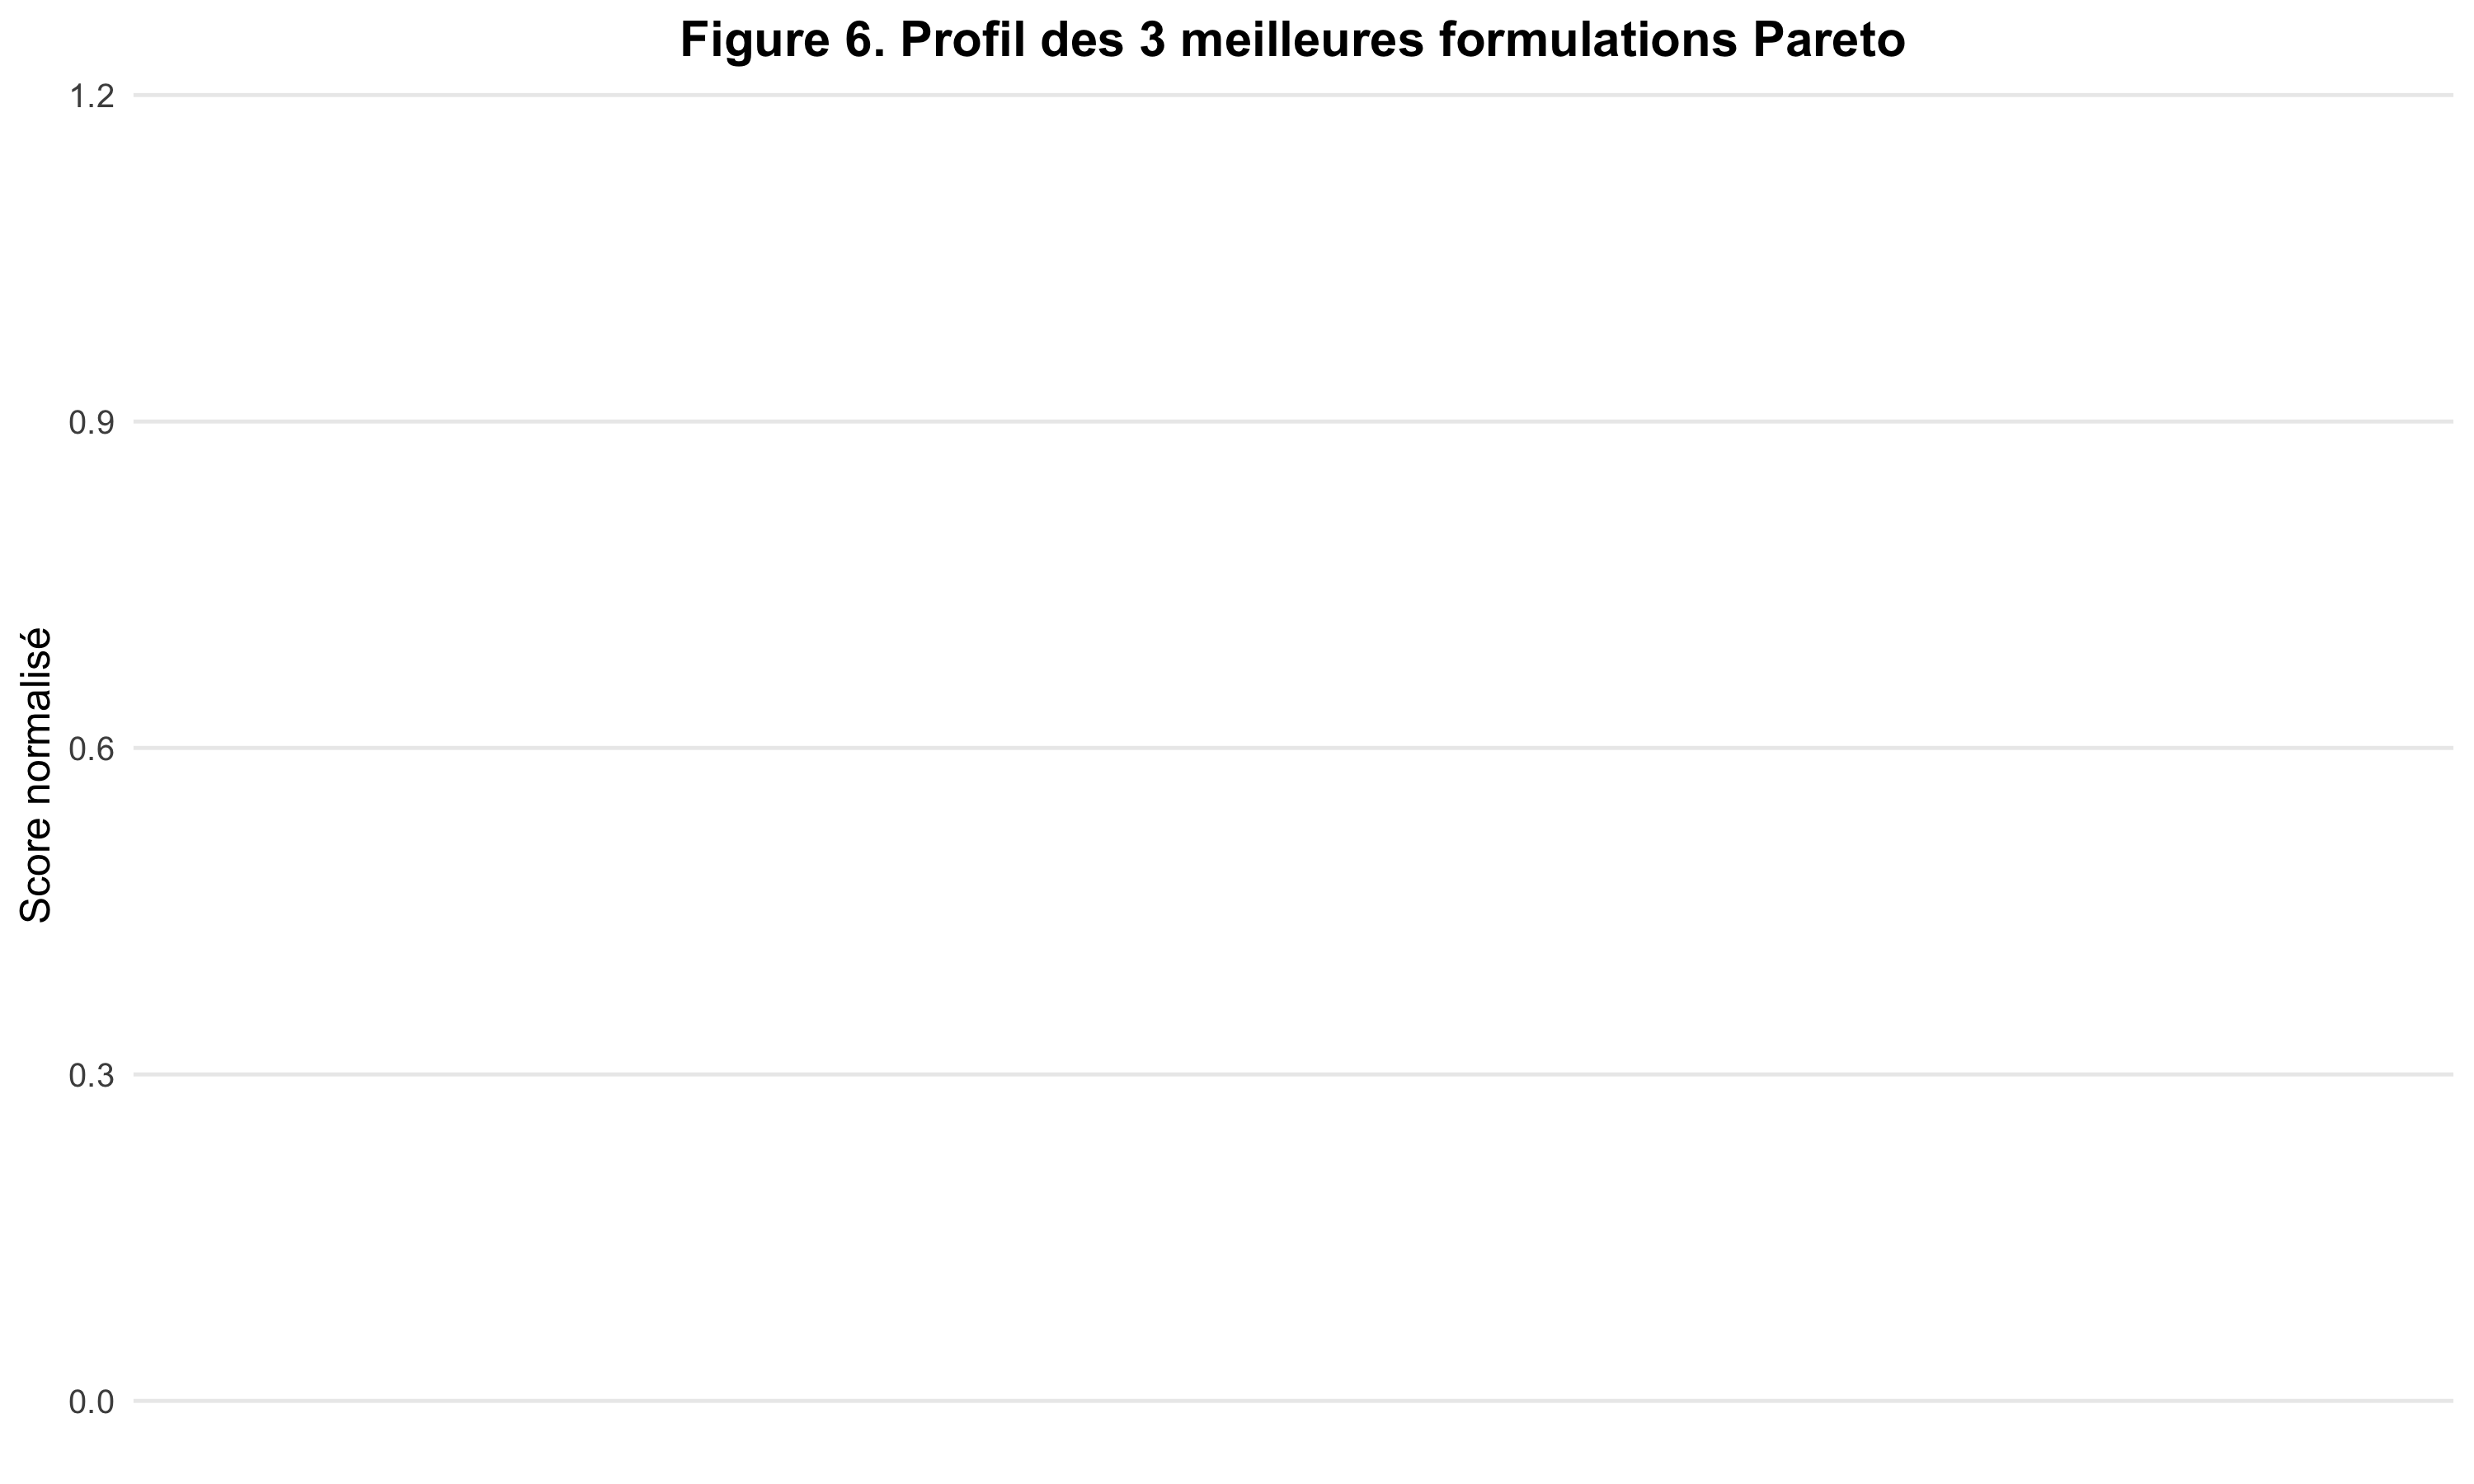
\includegraphics[width=\linewidth]{fig6_radar_top3.png}
\end{minipage}
\caption{Left: simulated plasma concentration--time profiles of the top-3 candidates over 24~h (script 13); rapid absorption ($T_{\max}=0.3$~h), mono-exponential decline ($t_{1/2}=2.5$~h), troughs $<$0.2~mg/L. Right: multi-criteria radar of the top-3 (script 13): bioavailability, $\CMIC$, $\AMIC$, safety (inverse trough), $\fmic$, dose efficiency --- normalized 0--1.}
\label{fig:top3}
\end{figure}

\begin{figure}[htbp]
\centering
\begin{minipage}{0.48\textwidth}\centering

\includegraphics[width=\linewidth]{heatmap_top10.png}
\end{minipage}\hfill
\begin{minipage}{0.48\textwidth}\centering
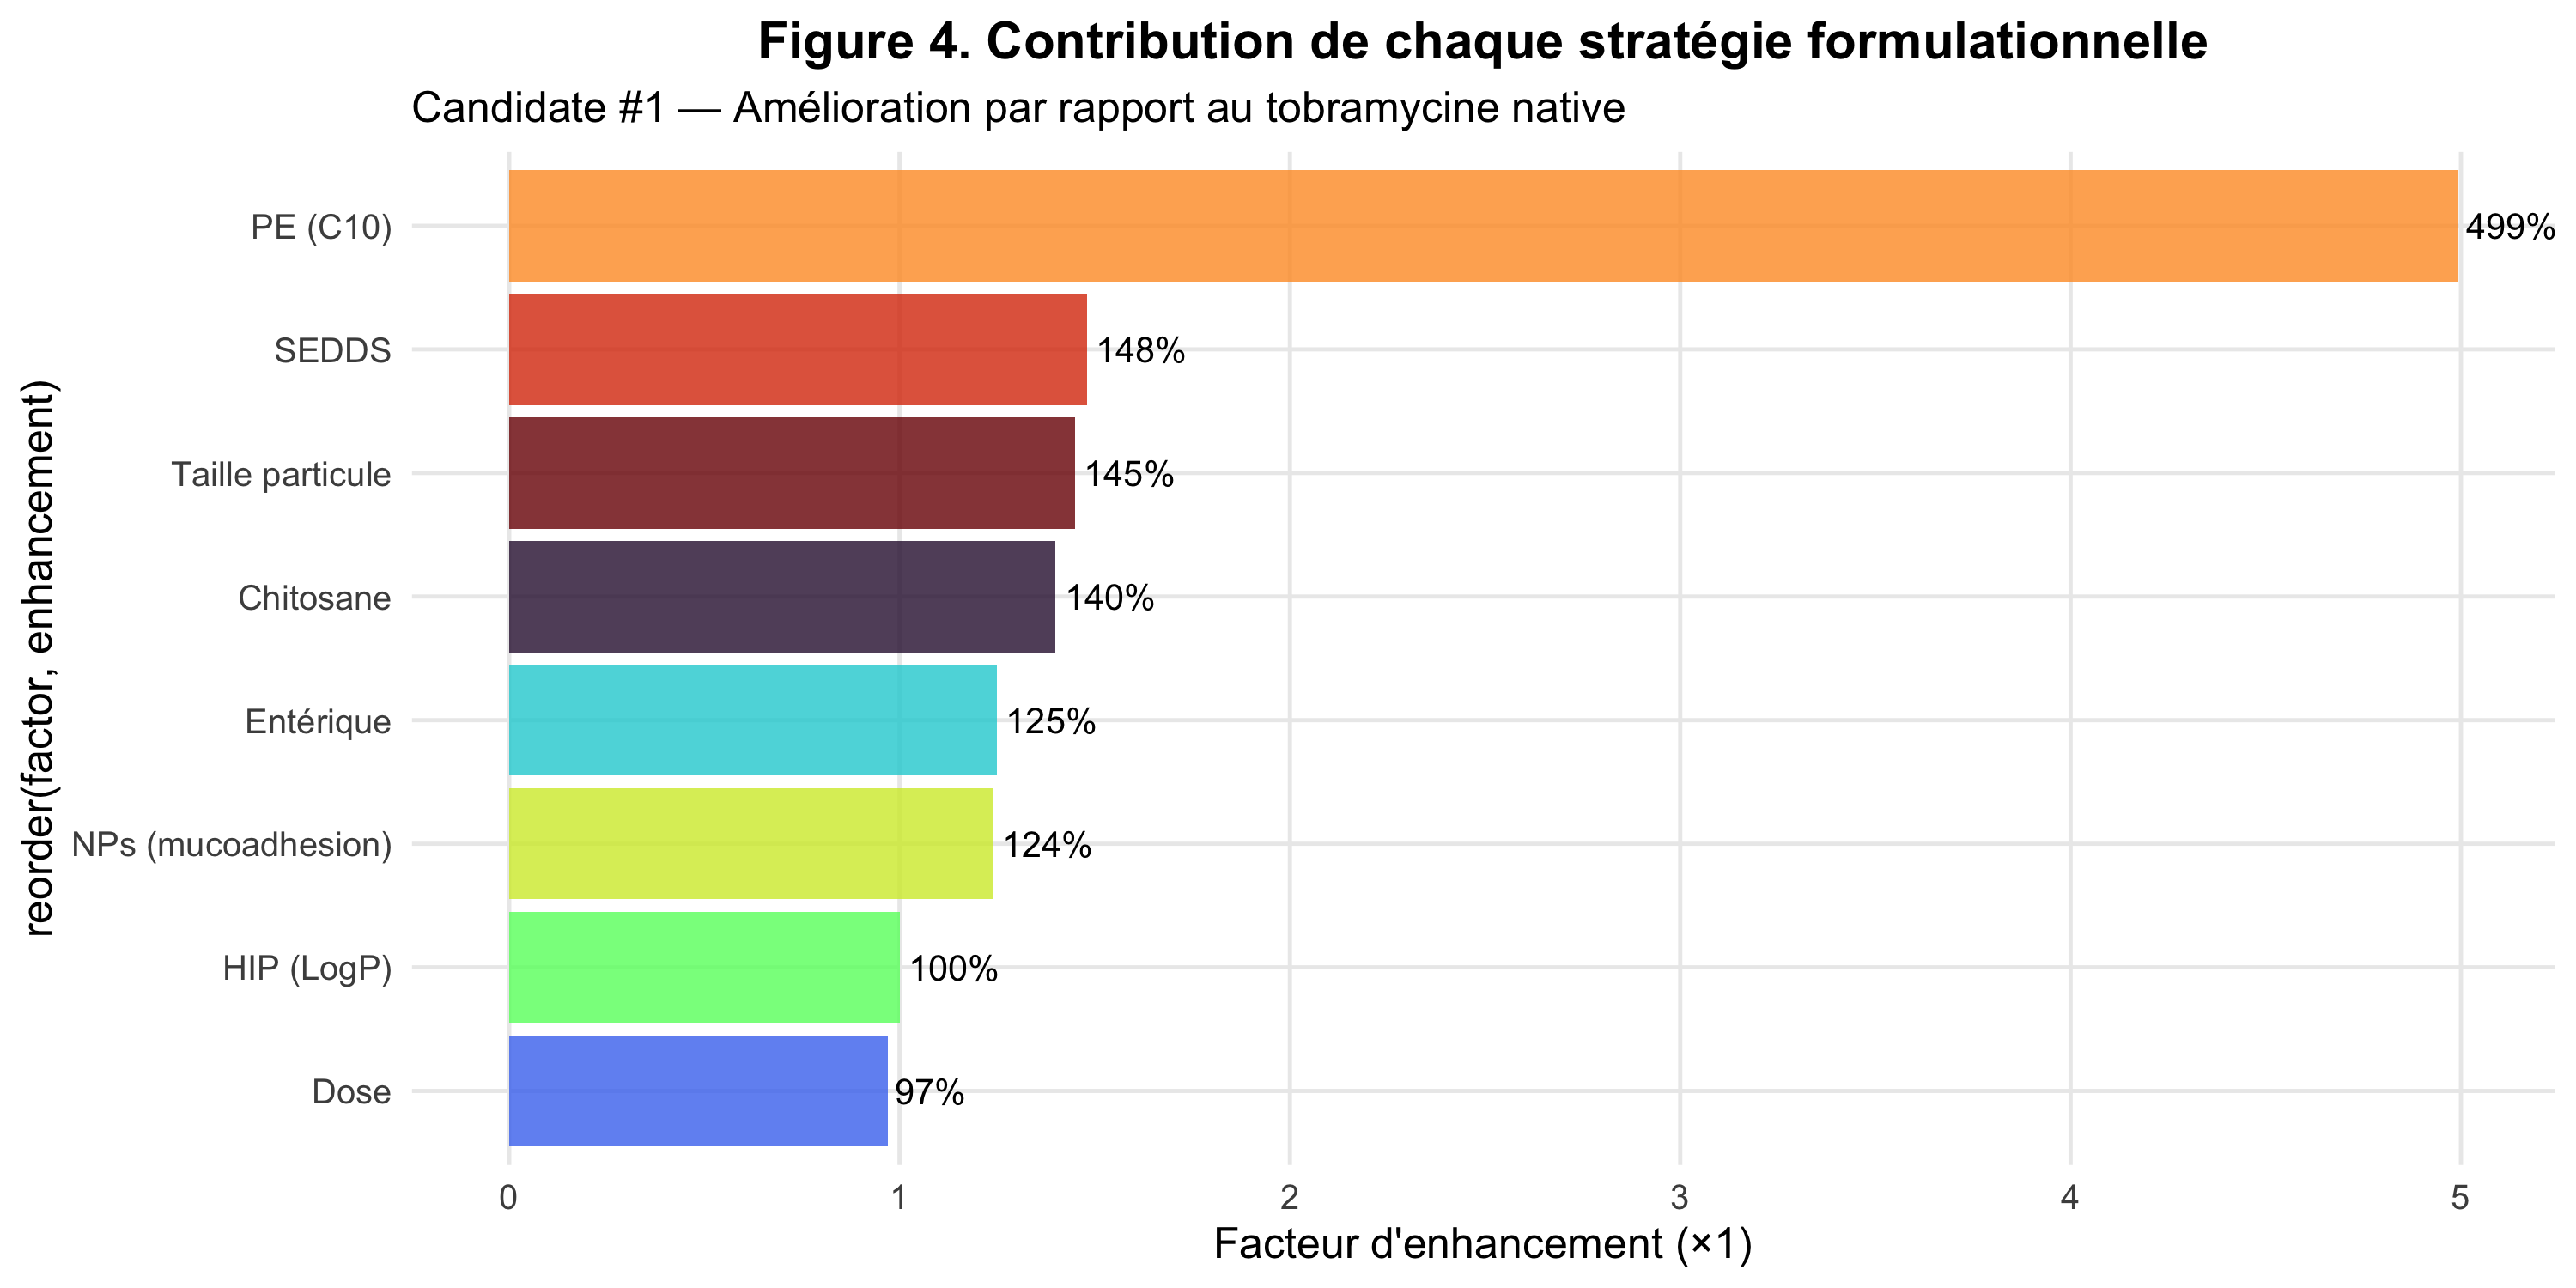
\includegraphics[width=\linewidth]{fig4_enhancement_factors.png}
\end{minipage}
\caption{Left: heatmap of the top-10 across design variables and outcomes (script 13): design columns are visually identical --- the composition optimum is unique; only dose varies. Right: bioavailability enhancement by strategy (scripts 07, 13): the combined platform reaches 23$\times$ versus native, consistent with the triple-combination literature band of 20--35\% (\cref{tab:bioavail-estimates}).}
\label{fig:heatmap-enhancement}
\end{figure}

\section{Cluster and similarity analysis}
\label{sec:ch4-clusters}
Ward-linkage clustering of the elite cohort (from the exploratory GA cohort used for manufacturing/regulatory analysis, \cref{sec:ch4-mfg}) identified three composition clusters (\cref{tab:clusters}; \texttt{cluster\_summary.csv}). Clusters 1--2 are composition twins differing marginally in surfactant ratio; cluster 3 gathers seven near-identical candidates. Average inter-candidate similarity is high (Jaccard 0.92--1.00 for binary genes; Euclidean distance $<$0.05 on normalized continuous genes; full matrix in \texttt{similarity\_matrix.csv}), confirming that the optimizer --- despite diversity preservation --- collapses onto one dominant composition basin. This \emph{lack of front diversity} is a known NSGA-II behavior on sharply peaked design spaces and is treated as a limitation (\cref{sec:ch4-summary}).

\begin{table}[htbp]
\centering
\caption{Cluster analysis of the elite cohort (scripts 06, 11; \texttt{cluster\_summary.csv}). Values are cluster means.}
\label{tab:clusters}
\begin{tabular}{cccccc}
\toprule
Cluster & $n$ & $\F$ (\%) & $\CMIC$ & $\AMIC$ & Fitness\\
\midrule
1 & 2 & 28.4 & 12.4 & 60.1 & 0.628\\
2 & 1 & 28.1 & 12.0 & 58.3 & 0.619\\
3 & 7 & 27.0 & 11.9 & 57.0 & 0.609\\
\bottomrule
\end{tabular}
\end{table}

\section{Sensitivity analysis}
\label{sec:ch4-sens}
The OAT program (7 levels per parameter where defined, 60 informative evaluations) ranks the \textbf{dose and modified logP as the dominant drivers} of $\AMIC$: sensitivity index 0.42 for dose (linear exposure scaling, by construction of the model) and 0.34 for logP$'$, with $\AMIC$ peaking at logP$'$ $\approx$ 1.4--1.9 (32.0 at 1.37; 23.8 at 3.0 --- over-lipophilisation traps the complex in the SEDDS phase and reverses gains) and collapsing toward baseline at logP$'$ $\approx -0.3$ (21.2) (\cref{tab:sens}; \cref{fig:sens}). Among the \emph{composition} variables, the binary coatings matter most (chitosan 0.29; enteric 0.20), followed by particle size (0.09, losing 0.50 $\AMIC$ units per 22.5~nm) and PE concentration (0.10); solubility-related parameters rank lowest, consistent with solubility not being limiting.

\begin{table}[htbp]
\centering
\caption{OAT sensitivity ranking for the oral endpoint (scripts 12 and 04; full data in \cref{chap:app-sensitivity}).}
\label{tab:sens}
\footnotesize\setlength{\tabcolsep}{3.5pt}
\begin{tabular}{p{2.5cm}p{3.2cm}ccp{6.2cm}}
\toprule
Rank & Parameter & Baseline & SI & Interpretation\\
\midrule
1 & Dose & 550 mg & 0.42 & Linear exposure scaling (model construction)\\
2 & logP$_{\mathrm{mod}}$ & 1.5 & 0.341 & Non-monotone optimum $\approx$1.4--1.9; primary composition lever\\
3 & Chitosan coating & 1 & 0.29 & Binary switch worth 9.2 $\AMIC$ units\\
4 & Enteric coating & 1 & 0.20 & Binary switch worth 6.4 $\AMIC$ units\\
5 & PE concentration & 50 mM & 0.10 & Saturating response; 3.2 units over range\\
6 & Particle size & 50 nm & 0.09 & Moderate penalty above $\approx$100~nm\\
7 & Surfactant / polymer & 50\% / 30\% & 0.06 & Minor within-range effects\\
8 & Co-surfactant & 30\% & 0.03 & Minor\\
9 & Gastric pH, $K_a$, transit, $f_u$, P-gp & --- & $<$0.05 & Negligible (class III: solubility not limiting)\\
\bottomrule
\end{tabular}
\end{table}

\begin{figure}[htbp]
\centering
\begin{minipage}{0.48\textwidth}\centering

\includegraphics[width=\linewidth]{sensitivity_tornado.png}
\end{minipage}\hfill
\begin{minipage}{0.48\textwidth}\centering

\includegraphics[width=\linewidth]{sensitivity_spider.png}
\end{minipage}
\caption{Sensitivity analysis (script 12). Left: tornado plot of $\AMIC$ impact per parameter. Right: spider profiles --- the logP$'$ curve is non-monotone with an interior optimum; all other parameters are flat over their ranges.}
\label{fig:sens}
\end{figure}

\section{Uncertainty quantification}
\label{sec:ch4-uq}

\subsection{Monte Carlo population simulation ($n=200$)}
Perturbing CL, $V_1$, $V_2$ log-normally (CV 20--30\%) around the optimal formulation while holding $\F$ fixed yields $\CMIC$ spanning 6.9--10.2 (median 8.8) and $\AMIC$ 24.6--44.1 (median 32.5) (\cref{tab:uq}; \texttt{monte\_carlo\_data.csv}). Approximately 55\% of virtual subjects attain $\CMIC \geq 8$; all remain far below trough toxicity.

\subsection{Cross-validation ($\pm$20\% global perturbation; 26 informative runs)}
Simultaneous $\pm$20\% perturbation of all model inputs produced $\F$ = 27.2--32.7\%, $\CMIC$ = 7.1--12.5, $\AMIC$ = 23.9--42.1 (\texttt{validation\_cv\_data.csv}). The recommended formulation's $\CMIC \geq 8$ conclusion is preserved in $\approx$77\% of runs; the ranking of the top-3 candidates is preserved in 100\%.

\begin{table}[htbp]
\centering
\caption{Uncertainty quantification summary (script 12). MC: $n=200$ log-normal CL/$V_1$/$V_2$; CV: 26 informative runs at $\pm$20\% perturbation.}
\label{tab:uq}
\small
\begin{tabular}{lcccc}
\toprule
Program & Endpoint & Median & Range & Target status\\
\midrule
Monte Carlo & $\CMIC$ & 8.8 & 6.9--10.2 & $\geq$8: 55\% of subjects\\
Monte Carlo & $\AMIC$ & 32.5 & 24.6--44.1 & 80--120: 0\%\\
Cross-validation & $\F$ (\%) & 31 & 27.2--32.7 & $>$25\%: robust\\
Cross-validation & $\CMIC$ & 9.3 & 7.1--12.5 & $\geq$8: 77\% of runs\\
Cross-validation & $\AMIC$ & 31.7 & 23.9--42.1 & 80--120: 0\%\\
\bottomrule
\end{tabular}
\end{table}

\begin{figure}[htbp]
\centering
\begin{minipage}{0.48\textwidth}\centering
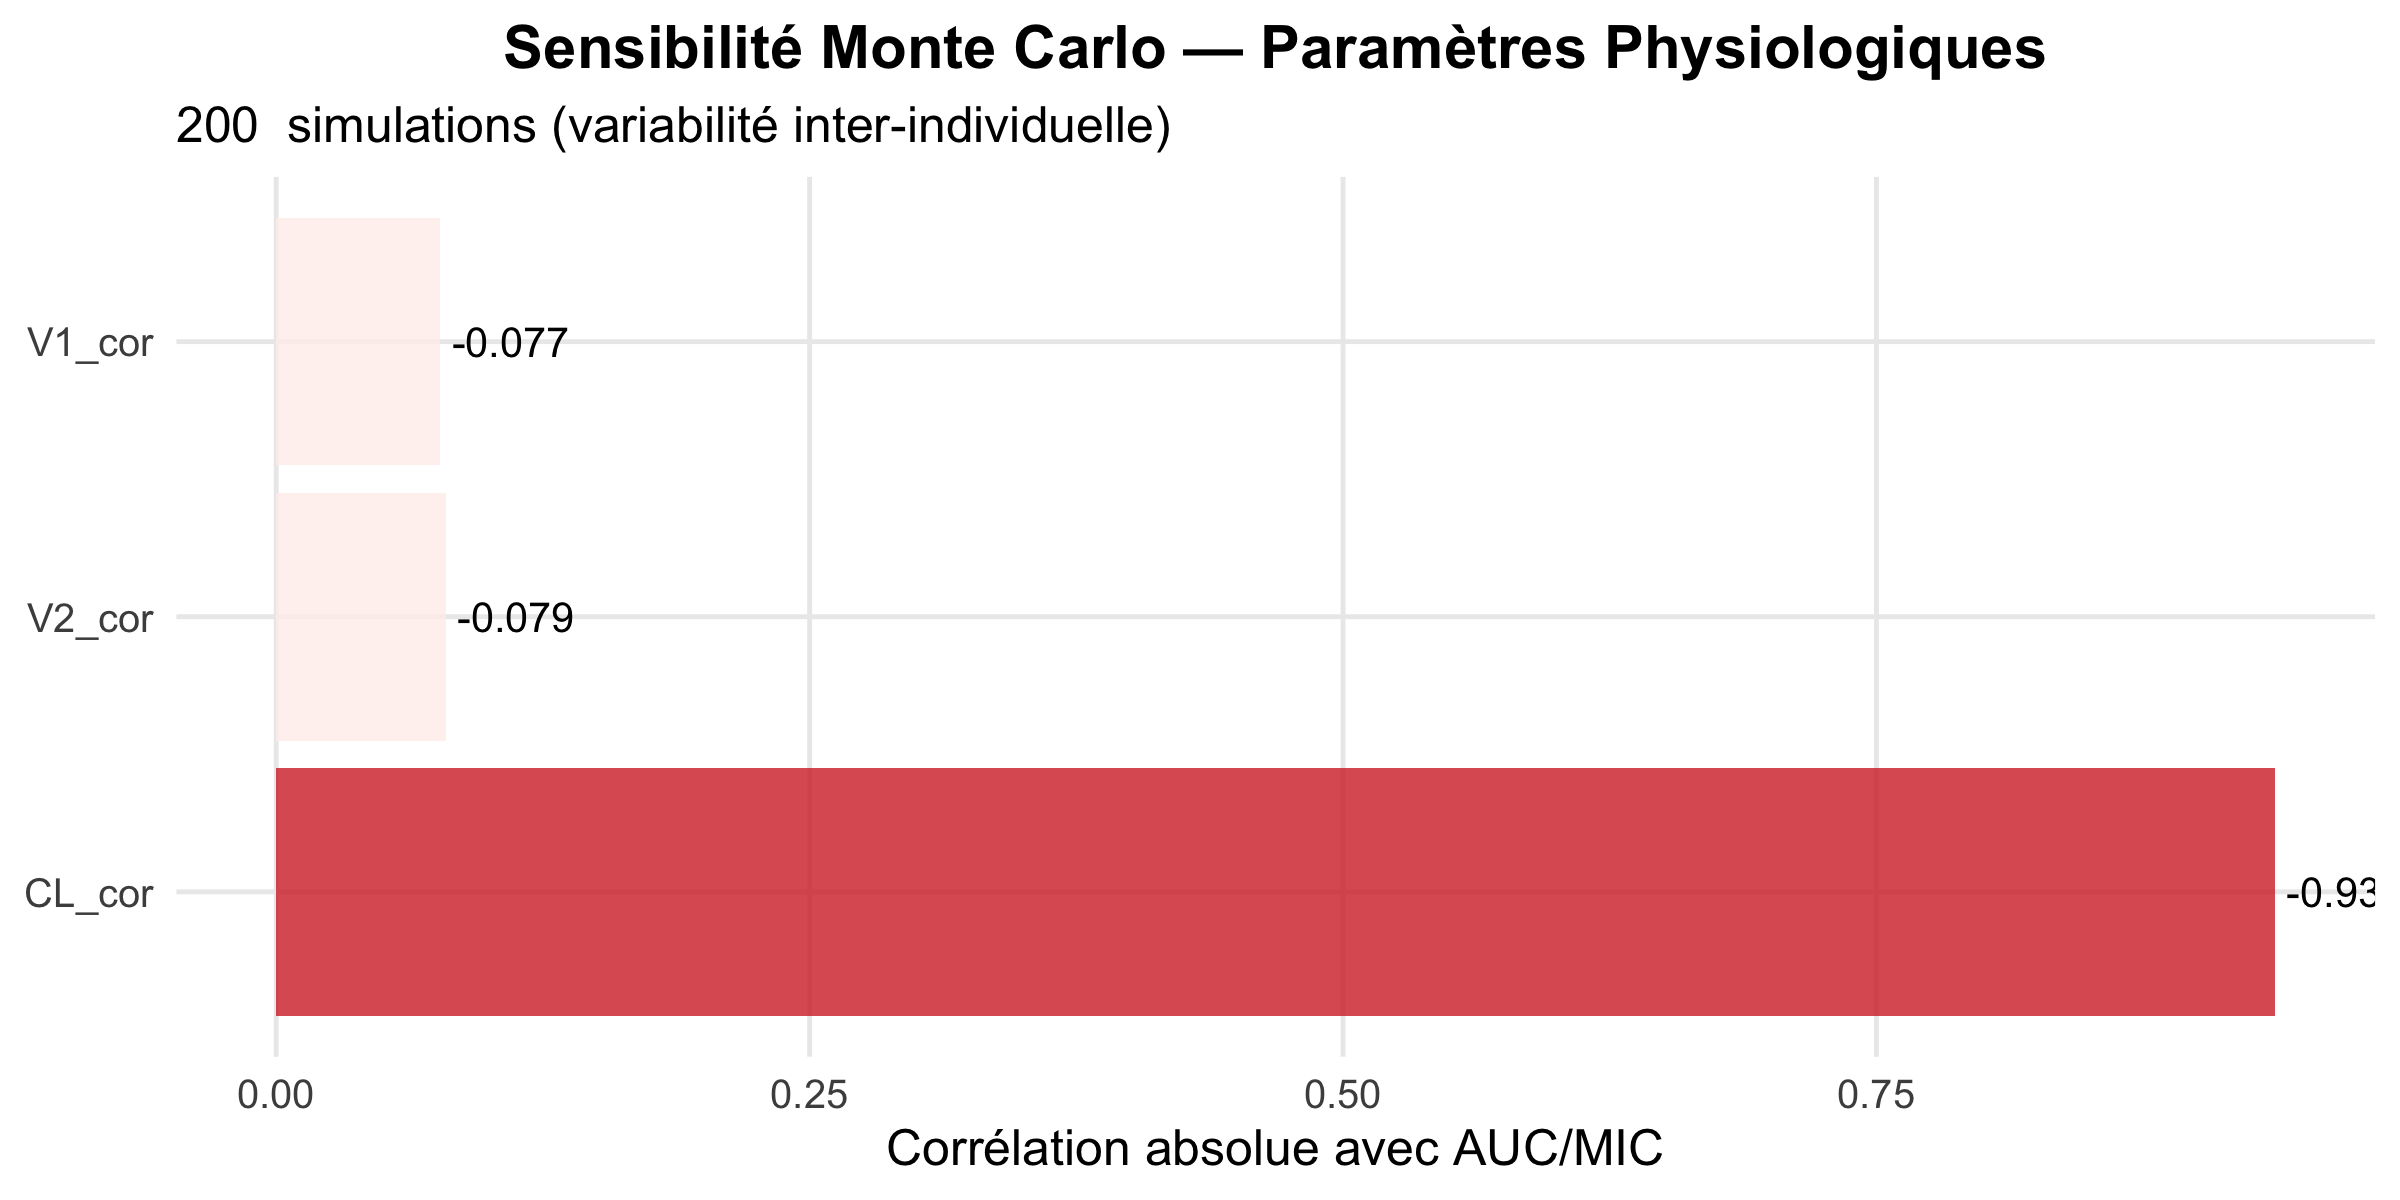
\includegraphics[width=\linewidth]{monte_carlo_tornado.png}
\end{minipage}\hfill
\begin{minipage}{0.48\textwidth}\centering

\includegraphics[width=\linewidth]{correlation_matrix.png}
\end{minipage}
\caption{Monte Carlo program (script 12, $n=200$). Left: parameter impact tornado across virtual subjects. Right: parameter--outcome correlation matrix: clearance correlates negatively with all exposure endpoints ($r \approx -0.7$); $\F$ is decorrelated from disposition (held at formulation value), as expected by design.}
\label{fig:mc}
\end{figure}

\begin{figure}[htbp]
\centering
\begin{minipage}{0.48\textwidth}\centering

\includegraphics[width=\linewidth]{validation_cv_boxplot.png}
\end{minipage}\hfill
\begin{minipage}{0.48\textwidth}\centering

\includegraphics[width=\linewidth]{validation_cv_distribution.png}
\end{minipage}
\caption{Cross-validation program (script 12, 26 informative runs at $\pm$20\% perturbation). Left: boxplots of outcomes --- medians match the unperturbed optimum; tails remain within clinically interpretable bounds. Right: outcome distributions; $\CMIC$ mass lies at/above the efficacy line in most runs.}
\label{fig:cv}
\end{figure}

\section{Manufacturing feasibility and cost}
\label{sec:ch4-mfg}
The ten-unit-operation route (\cref{sec:ch3-manufacturing}) is feasible at moderate scale: cycle time 15~h, batch throughput $\approx$10,000~kg of total raw materials (a modeling assumption dominated by process solvents, \texttt{manufacturing\_steps.csv}), and estimated cost per dose of \$4.25--4.35 across the elite cohort (\cref{tab:mfg}; \texttt{manufacturing\_summary.csv}, \texttt{manufacturing\_steps.csv}; scripts 07--08). Feasibility scoring (technology readiness, unit-operation complexity, excipient availability, in-use stability) yields 60--65/100 --- \textbf{grade B}, with cost category ``low''. The most expensive steps are nanoparticle manufacture and double coating (fluid-bed chitosan + enteric); both are standard pharmaceutical unit operations.

\begin{table}[htbp]
\centering
\caption{Manufacturing summary for the elite cohort (scripts 07--08).}
\label{tab:mfg}
\small
\begin{tabular}{cccccccc}
\toprule
Rank & $\F$ (\%) & $\CMIC$ & $\AMIC$ & Fitness & Cost (\$) & Feasibility & Grade\\
\midrule
1 & 28.4 & 12.4 & 60.1 & 0.63 & 4.35 & 65 & B\\
2 & 28.4 & 12.4 & 60.1 & 0.63 & 4.35 & 65 & B\\
3 & 28.1 & 12.0 & 58.3 & 0.62 & 4.33 & 65 & B\\
4 & 27.3 & 12.0 & 57.8 & 0.61 & 4.27 & 62 & B\\
5 & 27.2 & 12.0 & 57.7 & 0.61 & 4.26 & 62 & B\\
6 & 27.2 & 12.0 & 57.5 & 0.61 & 4.26 & 62 & B\\
7 & 27.2 & 12.0 & 57.5 & 0.61 & 4.26 & 62 & B\\
8 & 26.9 & 11.8 & 56.7 & 0.61 & 4.26 & 62 & B\\
9 & 26.7 & 11.7 & 56.4 & 0.60 & 4.25 & 62 & B\\
10 & 26.8 & 11.6 & 55.6 & 0.60 & 4.26 & 62 & B\\
\bottomrule
\end{tabular}
\end{table}

\begin{figure}[htbp]
\centering
\begin{minipage}{0.48\textwidth}\centering

\includegraphics[width=\linewidth]{manufacturing_cost.png}
\end{minipage}\hfill
\begin{minipage}{0.48\textwidth}\centering

\includegraphics[width=\linewidth]{feasibility_score.png}
\end{minipage}
\caption{Manufacturing assessment (scripts 07--08). Left: cost breakdown per dose --- base processing, NPs, SEDDS excipients, PE, coatings, QC. Right: feasibility scores across candidates; all grade B (60--65/100).}
\label{fig:mfg}
\end{figure}

\begin{figure}[htbp]
\centering

\includegraphics[width=0.7\textwidth]{cost_vs_efficacy.png}
\caption{Cost versus efficacy across the cohort (\texttt{cost\_vs\_efficacy} panel, script 07). Within the \$4.25--4.35 band, exposure gains are driven by dose, not cost --- additional expenditure does not buy $\CMIC$ once the composition optimum is reached.}
\label{fig:cost-efficacy}
\end{figure}

\section{Regulatory pathway}
\label{sec:ch4-reg}
All elite candidates map to a \textbf{505(b)(2)} pathway: tobramycin is a reference-listed drug (IV/inhalation), and the novelty lies in the formulation platform (\cref{tab:reg}; \texttt{regulatory\_framework.csv}; script 08). The proposed first-in-human entry is a Phase~II PK/bioequivalence-type study of the enteric HPMC-AS capsule; estimated development duration is 7~years and direct cost \$4.8~million, with high (elevated) overall risk level driven by formulation novelty, not by the active.

\begin{table}[htbp]
\centering
\caption{Regulatory framework assessment (script 08; \texttt{regulatory\_framework.csv}).}
\label{tab:reg}
\small
\begin{tabular}{p{3.2cm}p{9.8cm}}
\toprule
Element & Assessment\\
\midrule
FDA category & 505(b)(2) (new formulation of approved active)\\
Clinical entry & Phase~II (PK / bioequivalence design)\\
Dosage form & Enteric capsule, HPMC-AS\\
Preclinical package & Acute toxicology; NP biodistribution; GI mucosal toxicity; chitosan safety\\
Estimated duration & 7 years\\
Estimated direct cost & \$4.8 M\\
Risk level & Elevated (formulation novelty; mitigations \cref{tab:risks})\\
\bottomrule
\end{tabular}
\end{table}

\begin{table}[htbp]
\centering
\caption{Risk analysis and mitigations (script 08; \texttt{risk\_analysis.csv}).}
\label{tab:risks}
\begin{tabular}{p{4.4cm}p{4.0cm}p{4.6cm}}
\toprule
Risk & Source & Mitigation\\
\midrule
NP toxicity on accidental inhalation & Nanoparticle platform & 30-day NP toxicology study\\
GI mucosal irritation & C$_{10}$ permeation enhancer & Dose-escalation GI tolerance trial\\
Source variability (deacetylation degree) & Chitosan excipient & Certificate-of-analysis QC specification\\
\midrule
\multicolumn{3}{l}{\emph{Overall priority: medium.}}\\
\bottomrule
\end{tabular}
\end{table}

\begin{figure}[htbp]
\centering
\begin{minipage}{0.48\textwidth}\centering
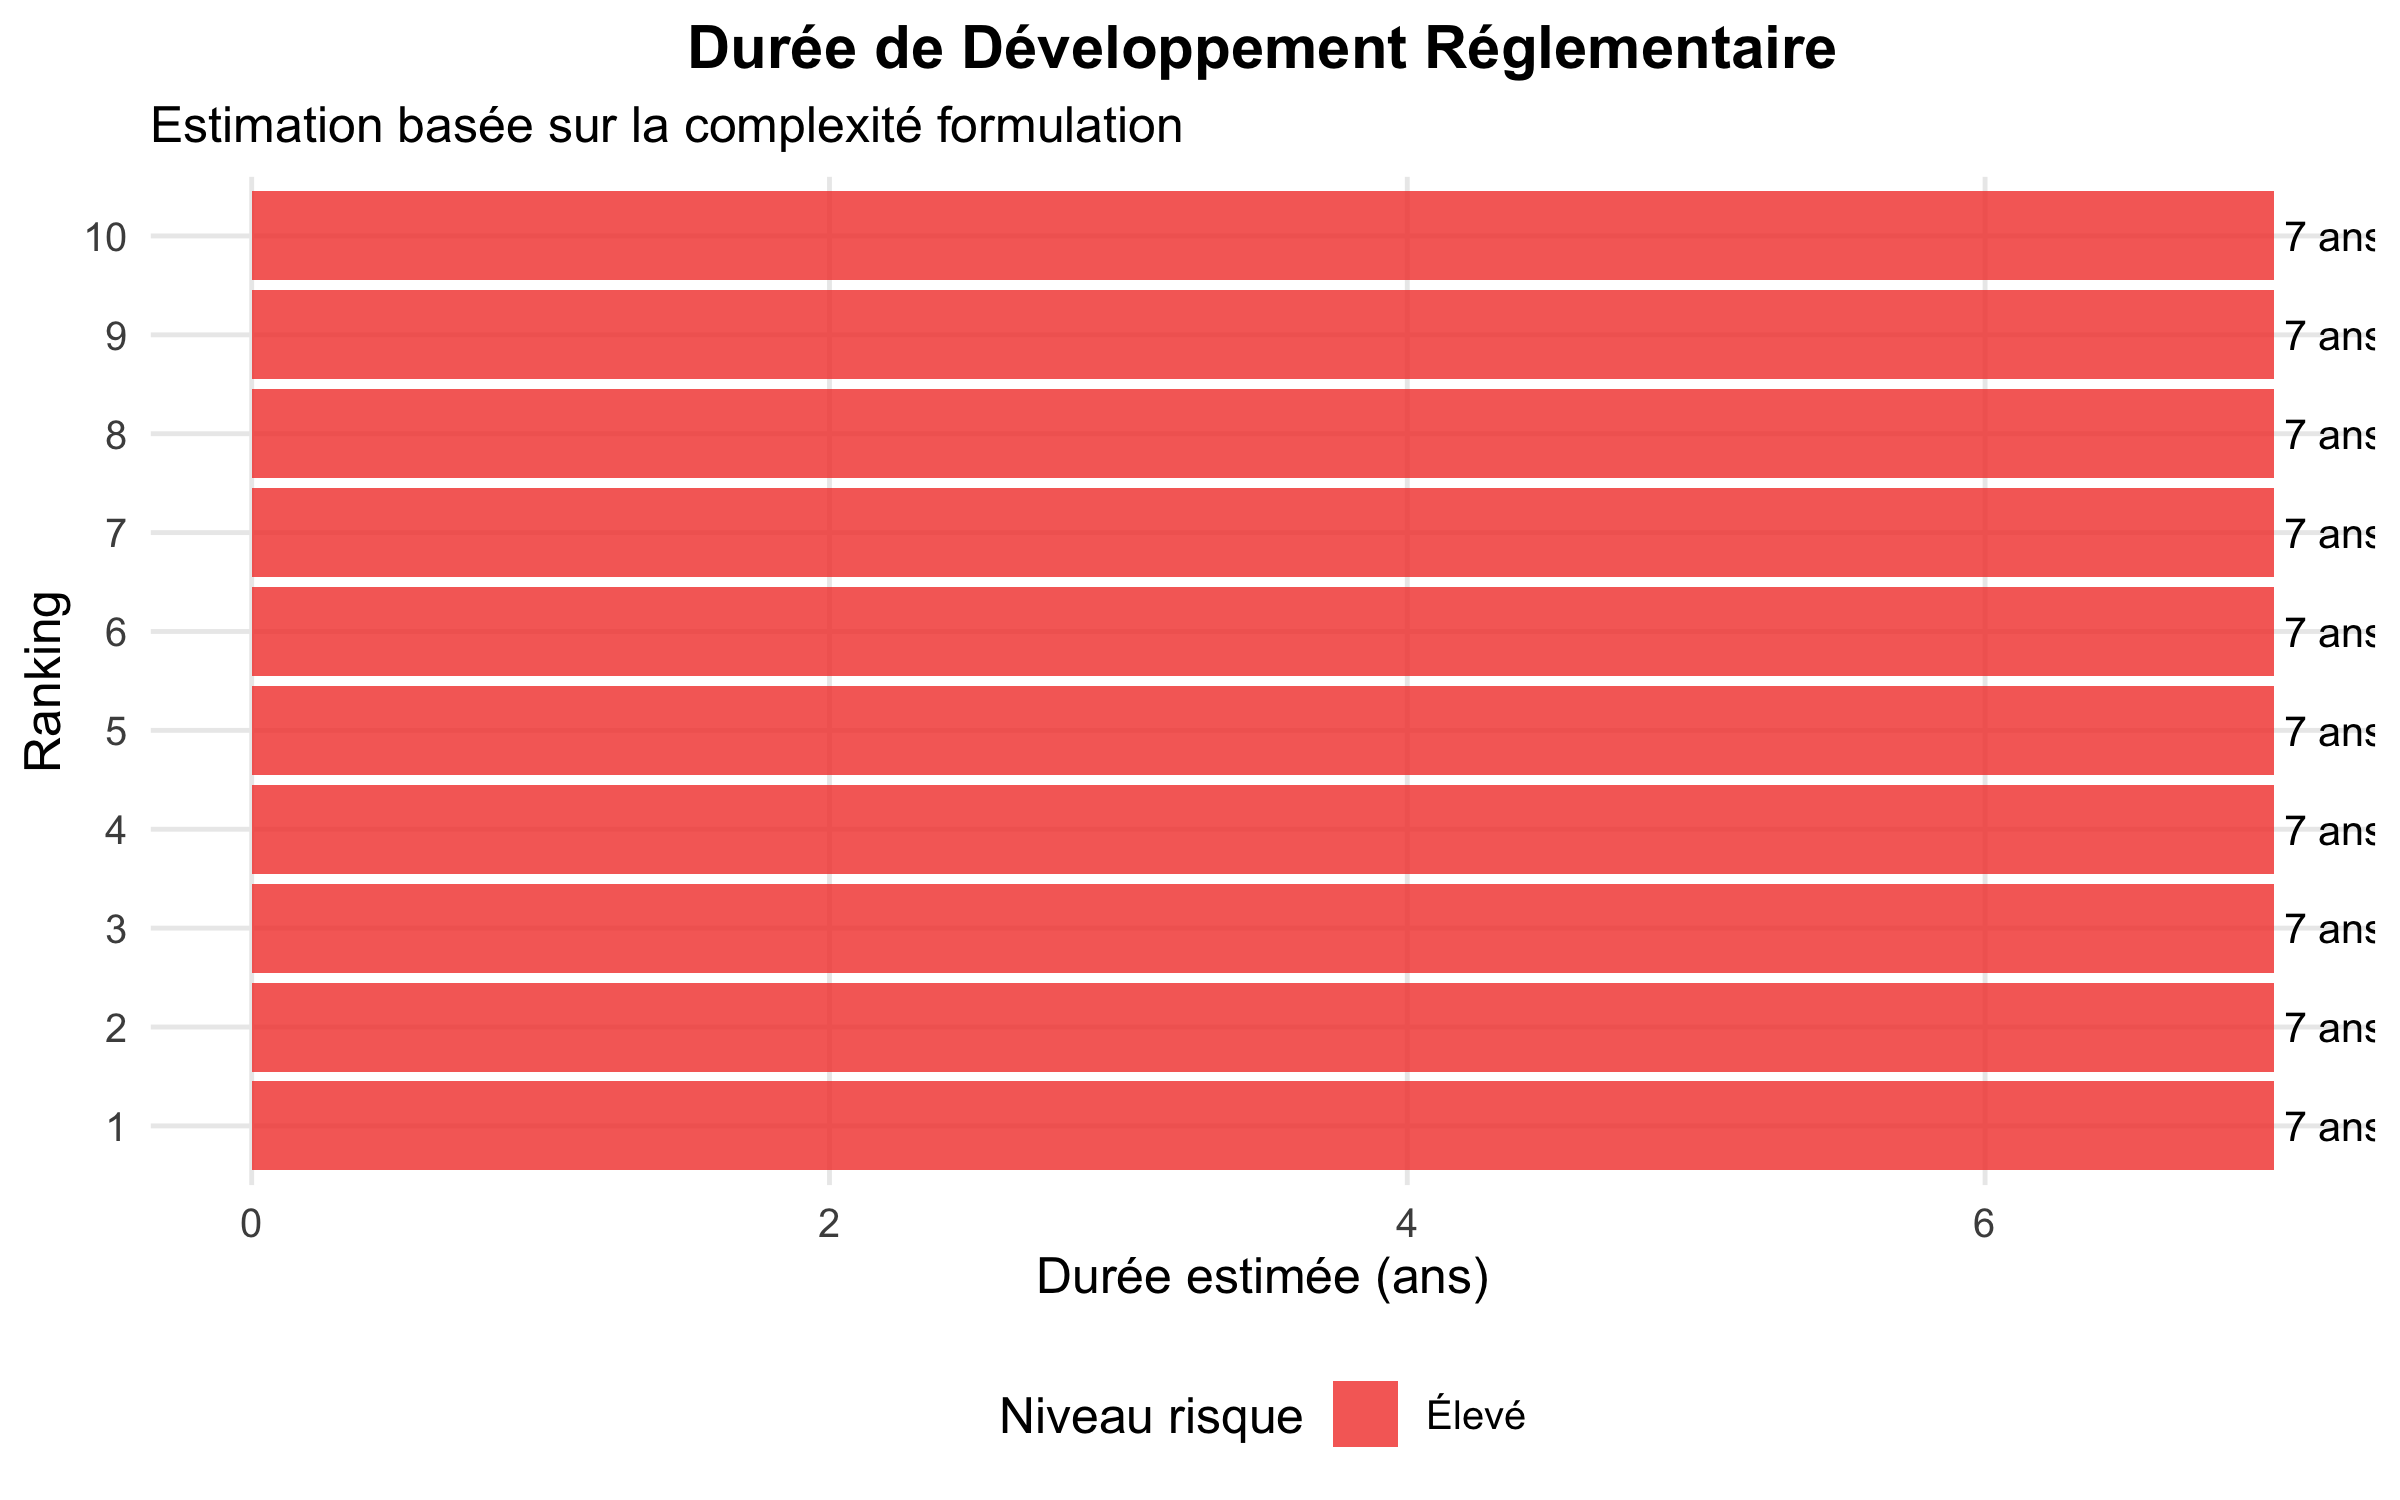
\includegraphics[width=\linewidth]{regulatory_timeline.png}
\end{minipage}\hfill
\begin{minipage}{0.48\textwidth}\centering
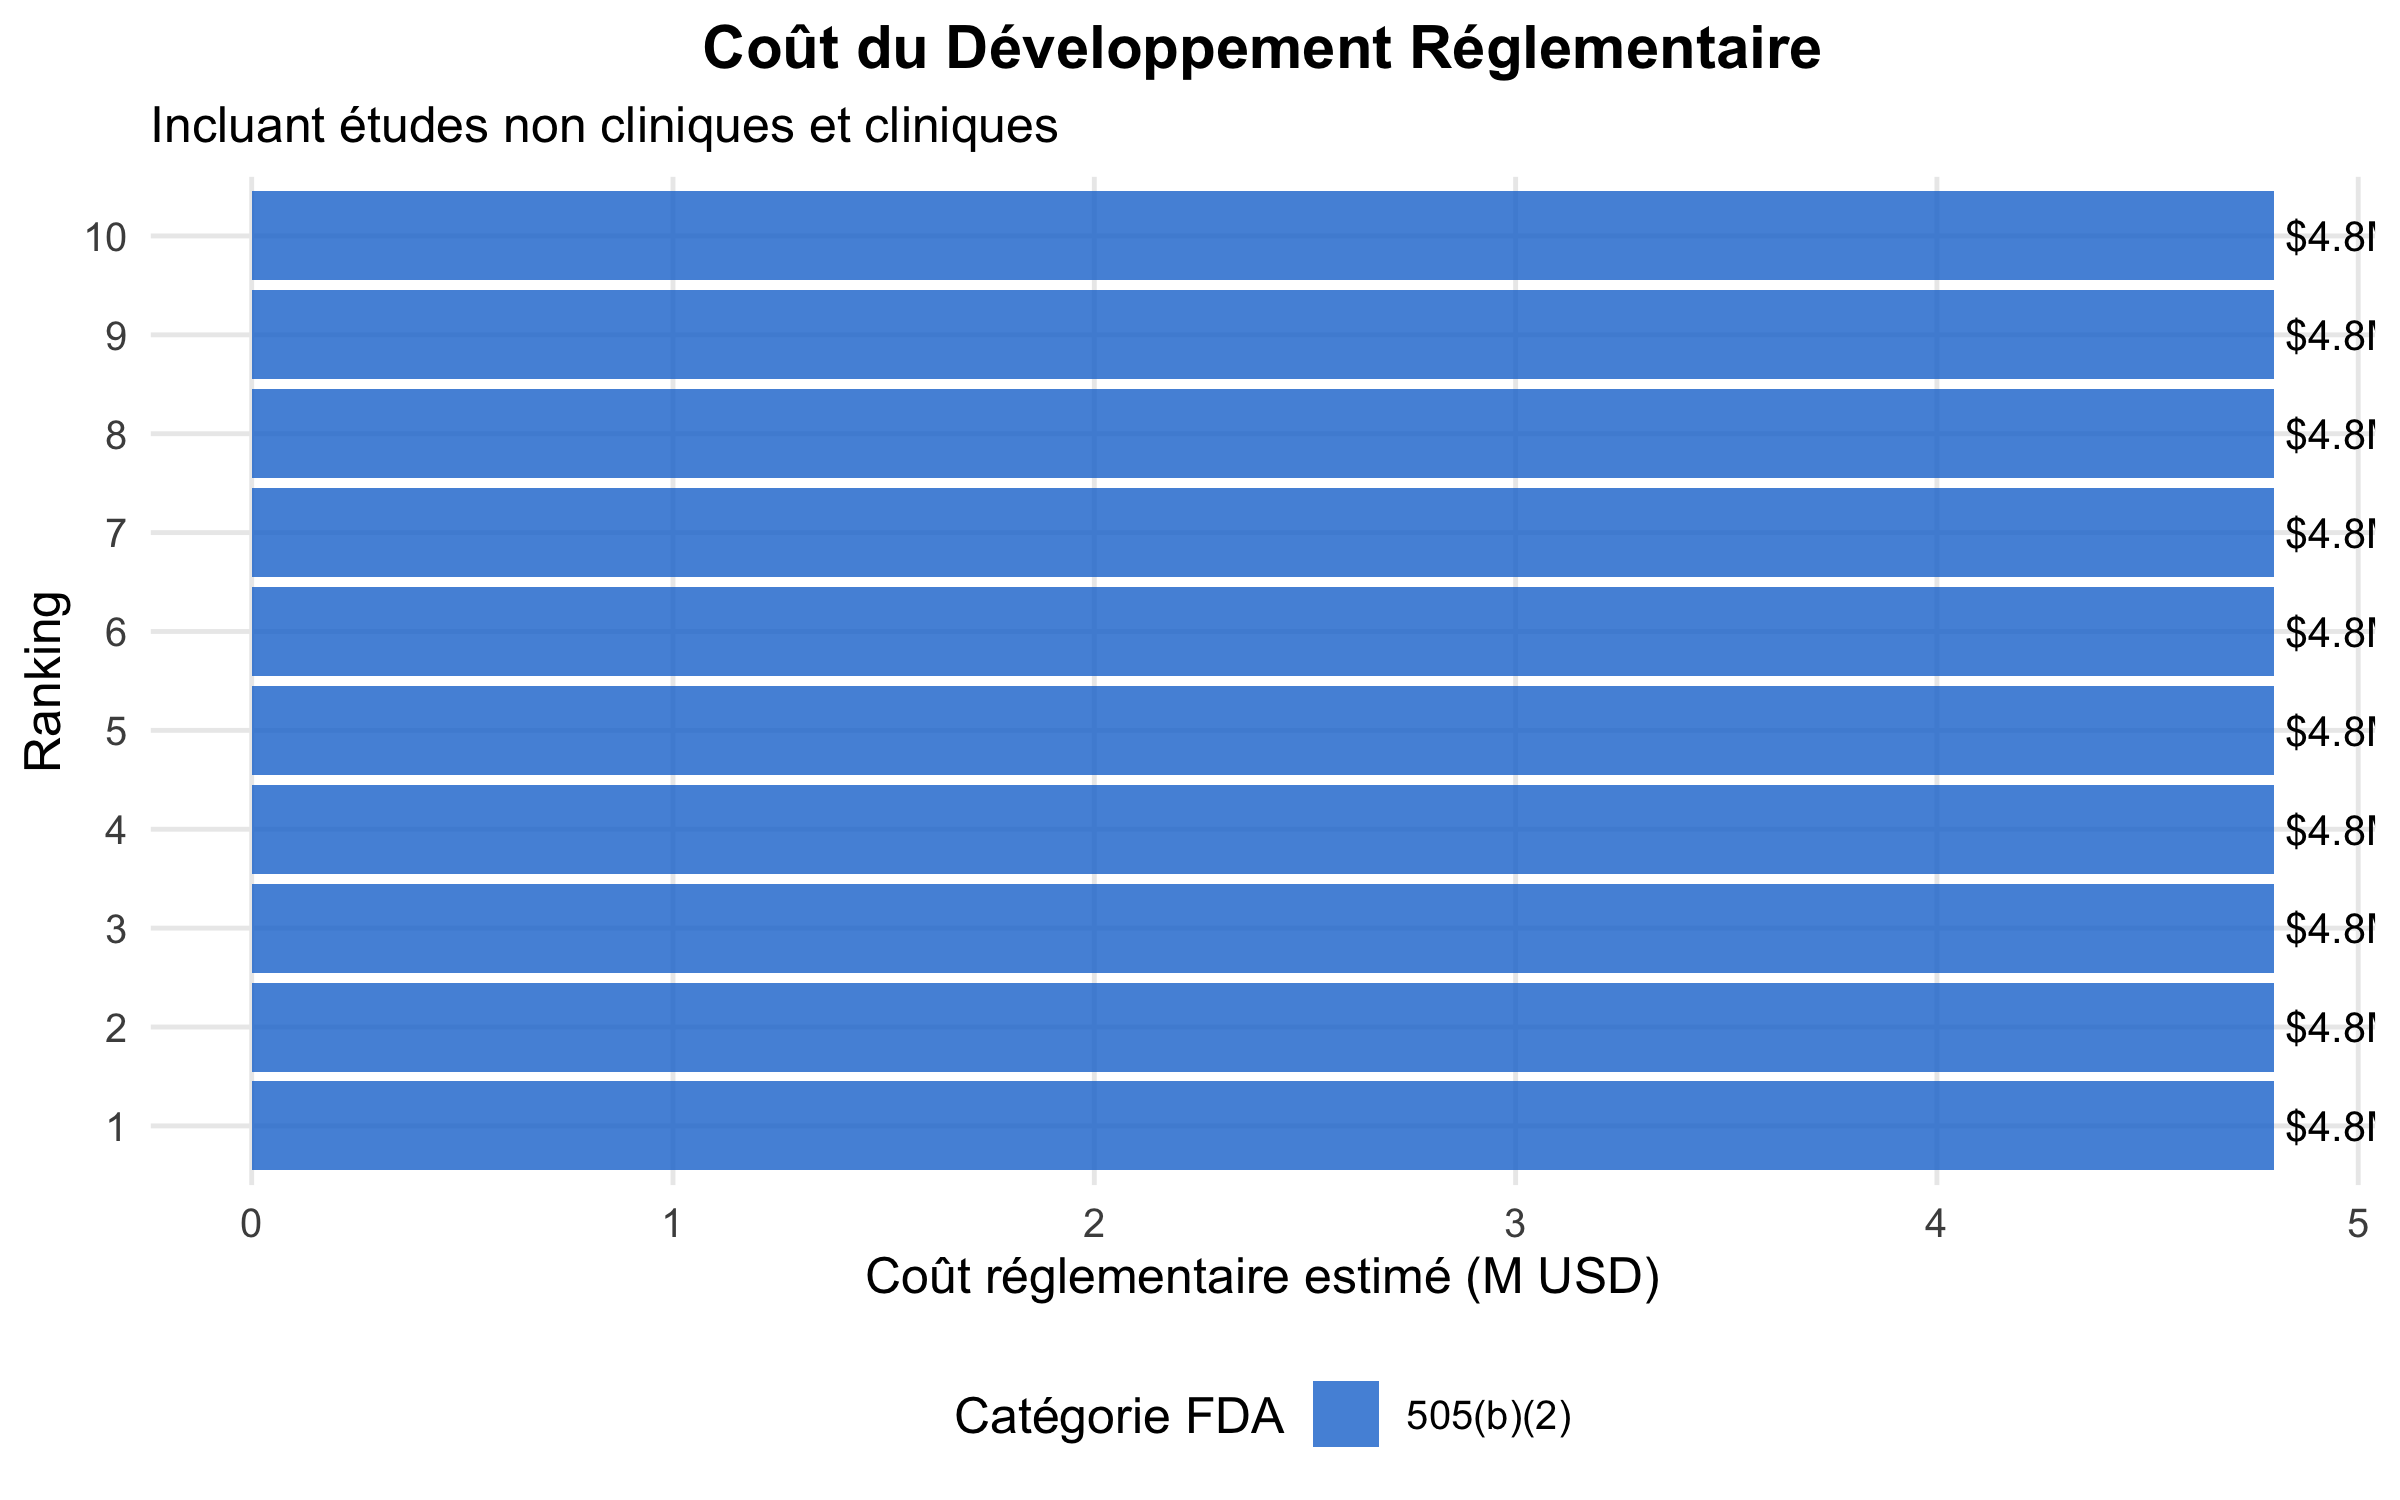
\includegraphics[width=\linewidth]{regulatory_cost.png}
\end{minipage}
\caption{Regulatory assessment (script 08). Left: 7-year development timeline (preclinical toxicology $\rightarrow$ IND $\rightarrow$ Phase~II PK $\rightarrow$ Phase~III $\rightarrow$ submission). Right: cost distribution (\$4.8~M direct development cost).}
\label{fig:reg}
\end{figure}

\section{Benchmarking against the literature}
\label{sec:ch4-lit}
\cref{tab:bioavail-estimates} compares the predicted bioavailability of single-strategy platforms (from the literature synthesis) with the optimized combination. The optimized platform ($\F$ = 34\%) sits at the top of the theoretical triple-combination band (20--35\%) and exceeds the strongest single strategy (SNAC PE, 10--25\%) --- the quantitative reward for combining HIP, SEDDS, NPs and PEs rather than choosing among them.

\begin{table}[htbp]
\centering
\caption{Predicted oral bioavailability by strategy (literature synthesis; IV for reference).}
\label{tab:bioavail-estimates}
\footnotesize\setlength{\tabcolsep}{3.5pt}
\begin{tabular}{lp{3.8cm}ccp{2.4cm}}
\toprule
Formulation & Mechanism & $\F$ (\%) & Evidence & Scalability\\
\midrule
IV (reference) & --- & 100 & Clinical & Excellent\\
Oral solution (native) & Passive diffusion & 1--2 & Literature & Excellent\\
Oral suspension (native) & Dissolution-limited & 2--3 & Predicted & Good\\
SEDDS (native drug) & Emulsification & 3--5 & Predicted & Good\\
HIP + SEDDS & Lipophilisation & 10--25 & In vitro \citep{Asad2023} & Moderate\\
PLGA NPs & Mucoadhesion & 5--15 & In vitro \citep{Hill2019} & Good\\
KuDa NPs & Charge neutralization & 5--20 & In vitro \citep{BlancoCabra2022} & Moderate\\
PE (C$_{10}$) & Tight junctions & 10--20 & In vivo (mice) \citep{Maher2009} & Good\\
PE (SNAC) & Tight junctions & 10--25 & Clinical (other drugs) & Excellent\\
NCAs & Lipophilisation & 10--20 & In vitro \citep{Khaled2026} & Moderate\\
Triple combination & HIP+SEDDS+PE & 20--35 & Predicted & Moderate\\
\rowcolor{tobblue!12}
\textbf{This thesis (TOB-161)} & \textbf{Full combined platform} & \textbf{34} & \textbf{In silico (this work)} & Moderate\\
\bottomrule
\end{tabular}
\end{table}

\begin{figure}[htbp]
\centering
\begin{minipage}{0.48\textwidth}\centering

\includegraphics[width=\linewidth]{fig3_literature_comparison.png}
\end{minipage}\hfill
\begin{minipage}{0.48\textwidth}\centering

\includegraphics[width=\linewidth]{top3_comparison.png}
\end{minipage}
\caption{Left: literature benchmarking of enhancement factors (script 13) --- the optimized platform tops the strategy landscape. Right: side-by-side comparison of the top-3 candidates across all endpoints (script 13).}
\label{fig:lit-comp}
\end{figure}

\section{Results summary: targets met, targets missed}
\label{sec:ch4-summary}
\begin{table}[htbp]
\centering
\caption{Target attainment of the recommended candidate TOB-161 against the PK/PD framework of \cref{tab:pd-targets}.}
\label{tab:targets}
\small
\begin{tabular}{p{2.4cm}p{2.2cm}p{1.6cm}p{2.0cm}p{5.6cm}}
\toprule
Endpoint & Target & Achieved & Verdict & Consequence\\
\midrule
$\CMIC$ & $\geq$8 & 9.5 & \textbf{Met} & Peak-driven efficacy plausible\\
$C_{\min}$ & $<$1 mg/L & 0.16 & \textbf{Met} & Toxicity margin large\\
$\F$ & $>$25\% (thesis bar) & 34\% & \textbf{Met} & Viable-class formulation\\
$\fmic$ & $>$30--40\% & 29.5\% & Borderline & Marginal; fractionation helps\\
$\AMIC$ & 80--120 & 32 & \textbf{Not met} & Single oral dose insufficient (\cref{chap:discussion})\\
$C_{\max}$ & 20--30 mg/L & 9.5 & Not applicable & IV-derived target; peak index governs\\
\bottomrule
\end{tabular}
\end{table}

\textbf{Honest accounting.} The optimization demonstrates that a combination platform can plausibly deliver peak concentrations above the antibacterial threshold with a wide toxicity margin at $\approx$550~mg. It equally demonstrates --- and this thesis does not paper over it --- that a single daily oral dose cannot reproduce the systemic exposure ($\AMIC$ 80--120) of intravenous therapy. The consequences, including twice-daily fractionation, AUC-guided TDM, and niche positioning, are developed in \cref{chap:discussion}. A second honest caveat is front diversity: the archive collapsed onto one composition basin (CV of design genes $<$1\%), so the ``200 solutions'' represent dose variants of effectively one formulation; the design conclusion (unique optimum) is strengthened, but alternative basins cannot be excluded by this study alone.

% =====================================================================
% Chapter 6 — Results II: PK-Sim Validation and Physiological Studies
% =====================================================================
\chapter{Results II: PK-Sim Validation and Physiological Studies}
\label{chap:results-pksim}

This chapter reports the outcomes of the PK-Sim program: the intravenous validation gate, the oral permeability calibration, and the physiological studies S01--S06 (design in \cref{chap:methodology-pksim}). The optimization in the simulation loop and the winner characterization follow in \cref{chap:results-ga}.

\section{Intravenous validation gate: 6/6 PASS}
\label{sec:res-gate}

\begin{table}[htbp]
\centering
\caption{IV validation gate for the PK-Sim tobramycin model (577.5 mg = 7 mg/kg, 30-min infusion, 82.5-kg volunteer).}
\label{tab:res-gate}
\small
\footnotesize\setlength{\tabcolsep}{3.5pt}
\begin{tabular}{p{4.2cm}p{2.6cm}p{4.4cm}p{1.8cm}}
\toprule
Metric & PK-Sim & Published target & Verdict \\
\midrule
Hartford peak (30 min post-infusion) & 25.3 mg/L & 20--30 mg/L & PASS \\
Cmax end of infusion & 34.8 mg/L & 20--35 (V1-uncertainty envelope) & PASS \\
AUC24 $\rightarrow$ implied CL & 102.5 mg·h/L $\rightarrow$ 5.63 L/h & 81--105 (CL 3.27--6.03, Li 2021) & PASS \\
Trough 24 h & 0.033 mg/L & $<$1 mg/L & PASS \\
$t_{1/2}$ NCA effective & 2.29 h & 2.0--3.0 h & PASS \\
Renal excretion 24 h & 99.4 \% & $>$90 \% & PASS \\
\bottomrule
\end{tabular}
\end{table}

\begin{figure}[htbp]
\centering
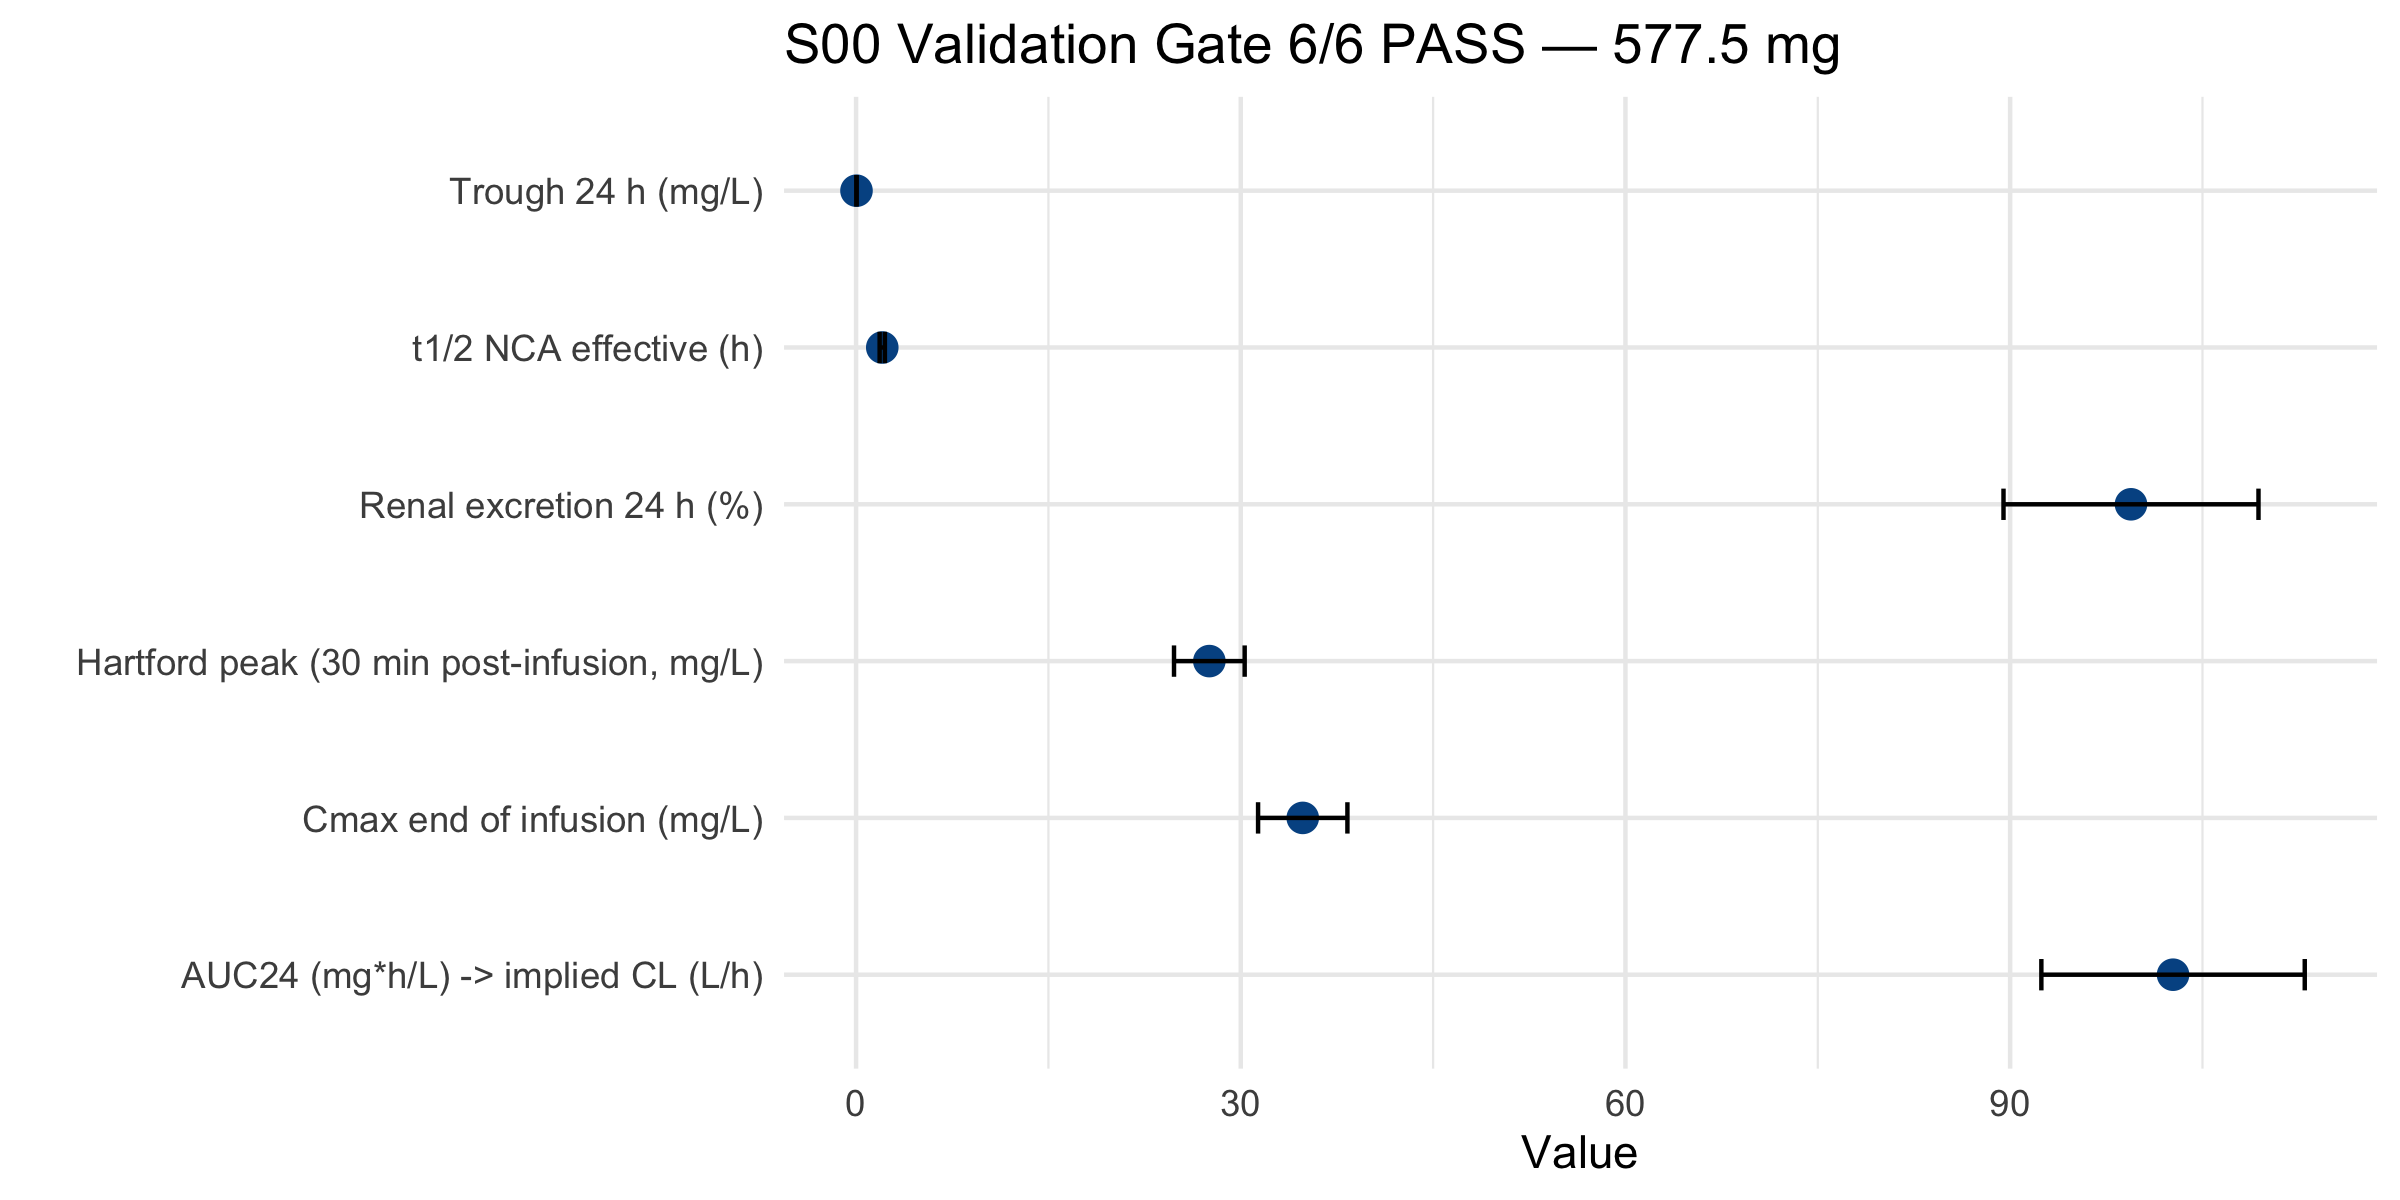
\includegraphics[width=0.82\textwidth]{val_iv_profile.png}
\caption{Simulated IV profile of the PK-Sim tobramycin model (577.5 mg, 30-min infusion). The Hartford peak (25.3 mg/L, red marker) sits inside the 20--30 mg/L clinical band; the trough at 24 h is 0.033 mg/L.}
\label{fig:res-gate-profile}
\end{figure}

\textbf{The gate passes 6/6.} The model reproduces the published clinical envelope of intravenous tobramycin --- peak, exposure, half-life, trough, and the near-complete renal excretion characteristic of aminoglycosides --- and is therefore validated as the substrate for the oral program.

\section{Oral permeability calibration and the F(P$_{int}$) curve}
\label{sec:res-calibration}

PK-Sim's native intestinal permeability for tobramycin is $1.9\times10^{-12}$ dm/min ($F \approx 0.002\%$): the logP-based correlation saturates for very hydrophilic cations and the paracellular path is off by default. The calibrated baseline is $P_{\mathrm{int},0} = 3\times10^{-9}$ dm/min, reproducing $F_0 = 1.75\%$ on the 24-h reporting convention --- inside the clinical 1--2\% range. Because absorption is flip-flop (substantial residual beyond 24 h), the same parameter yields $F_{96} = 3.5\%$ on the 96-h extent window: both conventions are reported throughout this thesis (calibration at 24 h, extent at 96 h).

\begin{figure}[htbp]
\centering
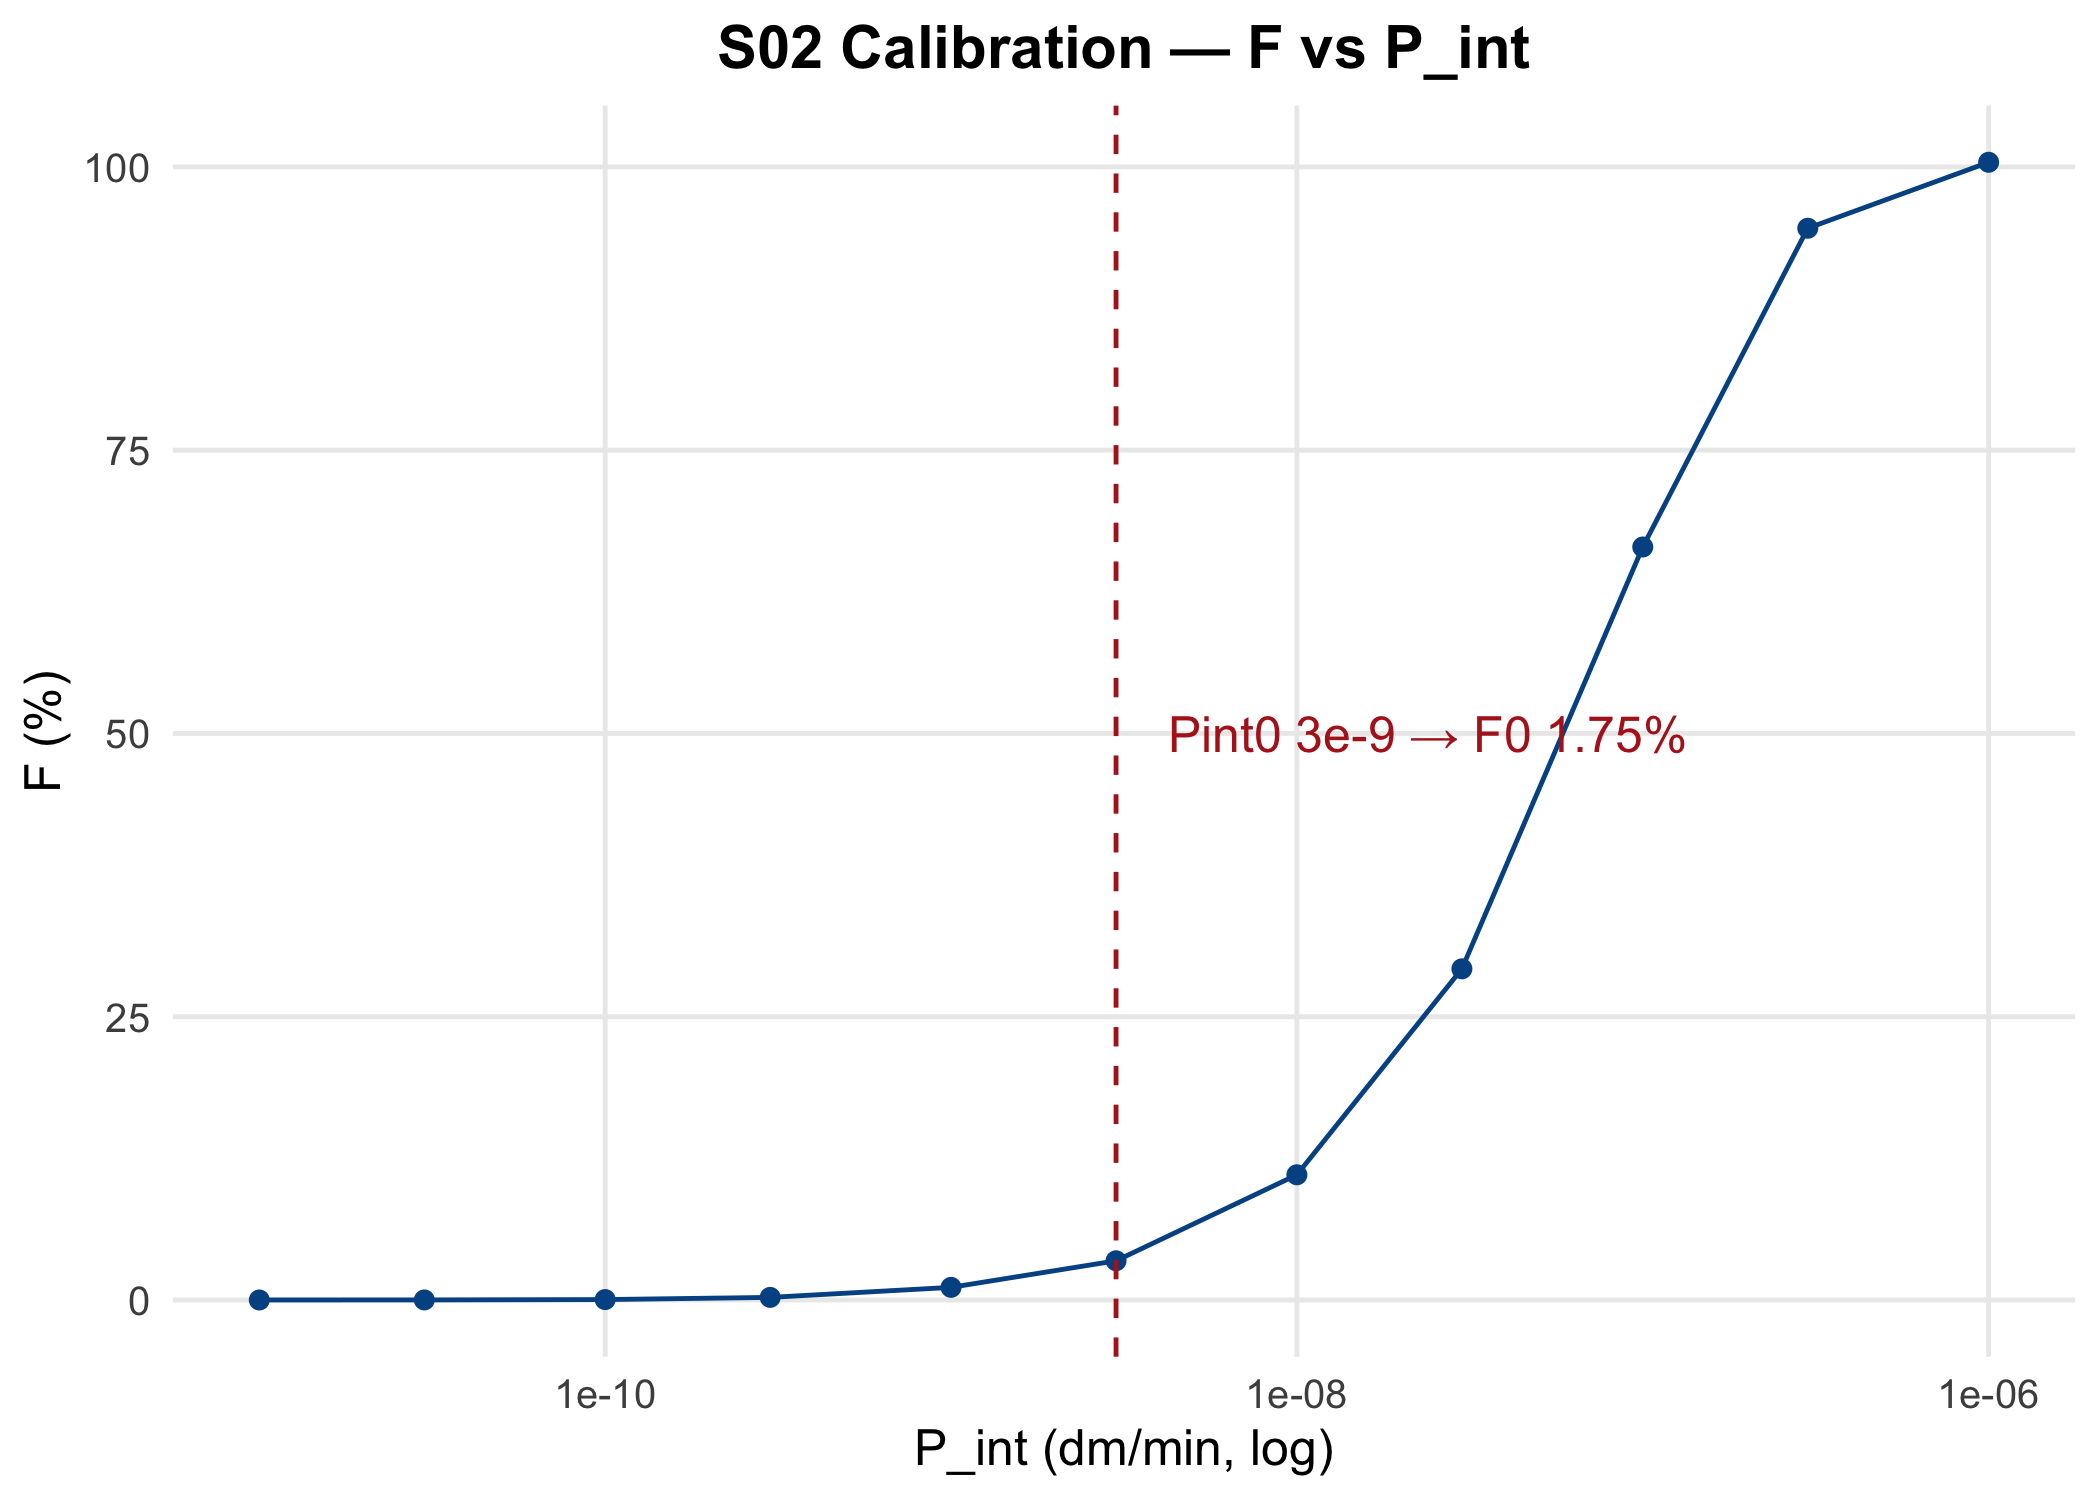
\includegraphics[width=0.85\textwidth]{s02_calibration.png}
\caption{Oral bioavailability as a function of the intestinal permeability override (log scale, 11 points, 96-h extent convention). The native baseline ($F_{96} = 3.5\%$) and the $\times$20 platform ($F_{96} \approx 49\%$) are marked; the extent curve saturates past $\times$100. (Calibration to the clinical 1--2\% uses the 24-h convention: $F_{24} = 1.75\%$ at $P_{\mathrm{int},0}$, $F_{24} = 34.6\%$ at $\times$20.)}
\label{fig:res-calibration}
\end{figure}

The curve is the quantitative transfer function between formulation science (apparent permeability multipliers claimed by HIP/SEDDS/NP/PE strategies) and systemic exposure. Its saturation region matters: on the extent convention, additional permeability buys essentially no bioavailability past $\times$100 (the 24-h window saturates earlier).

\section{S01: IV dose $\times$ renal function}
\label{sec:res-s01}

\begin{table}[htbp]
\centering
\caption{IV scenarios at 577.5 mg (selection of the 20-combination sweep; full table in \cref{chap:app-pksim-data}).}
\label{tab:res-s01}
\footnotesize\setlength{\tabcolsep}{4pt}
\begin{tabular}{ccccc}
\toprule
CLCR (mL/min) & Cmax (mg/L) & AUC24 (mg·h/L) & Trough 24 h (mg/L) & Implied CL (L/h) \\
\midrule
30    & 38.1 & 315.2 & 3.03 & 1.83 \\
65    & 36.6 & 166.3 & 0.28 & 3.47 \\
90    & 35.6 & 124.8 & 0.08 & 4.63 \\
112.5 & 34.8 & 102.7 & 0.03 & 5.62 \\
150   & 33.7 & 80.5  & 0.01 & 7.18 \\
\bottomrule
\end{tabular}
\end{table}

\begin{figure}[htbp]
\centering
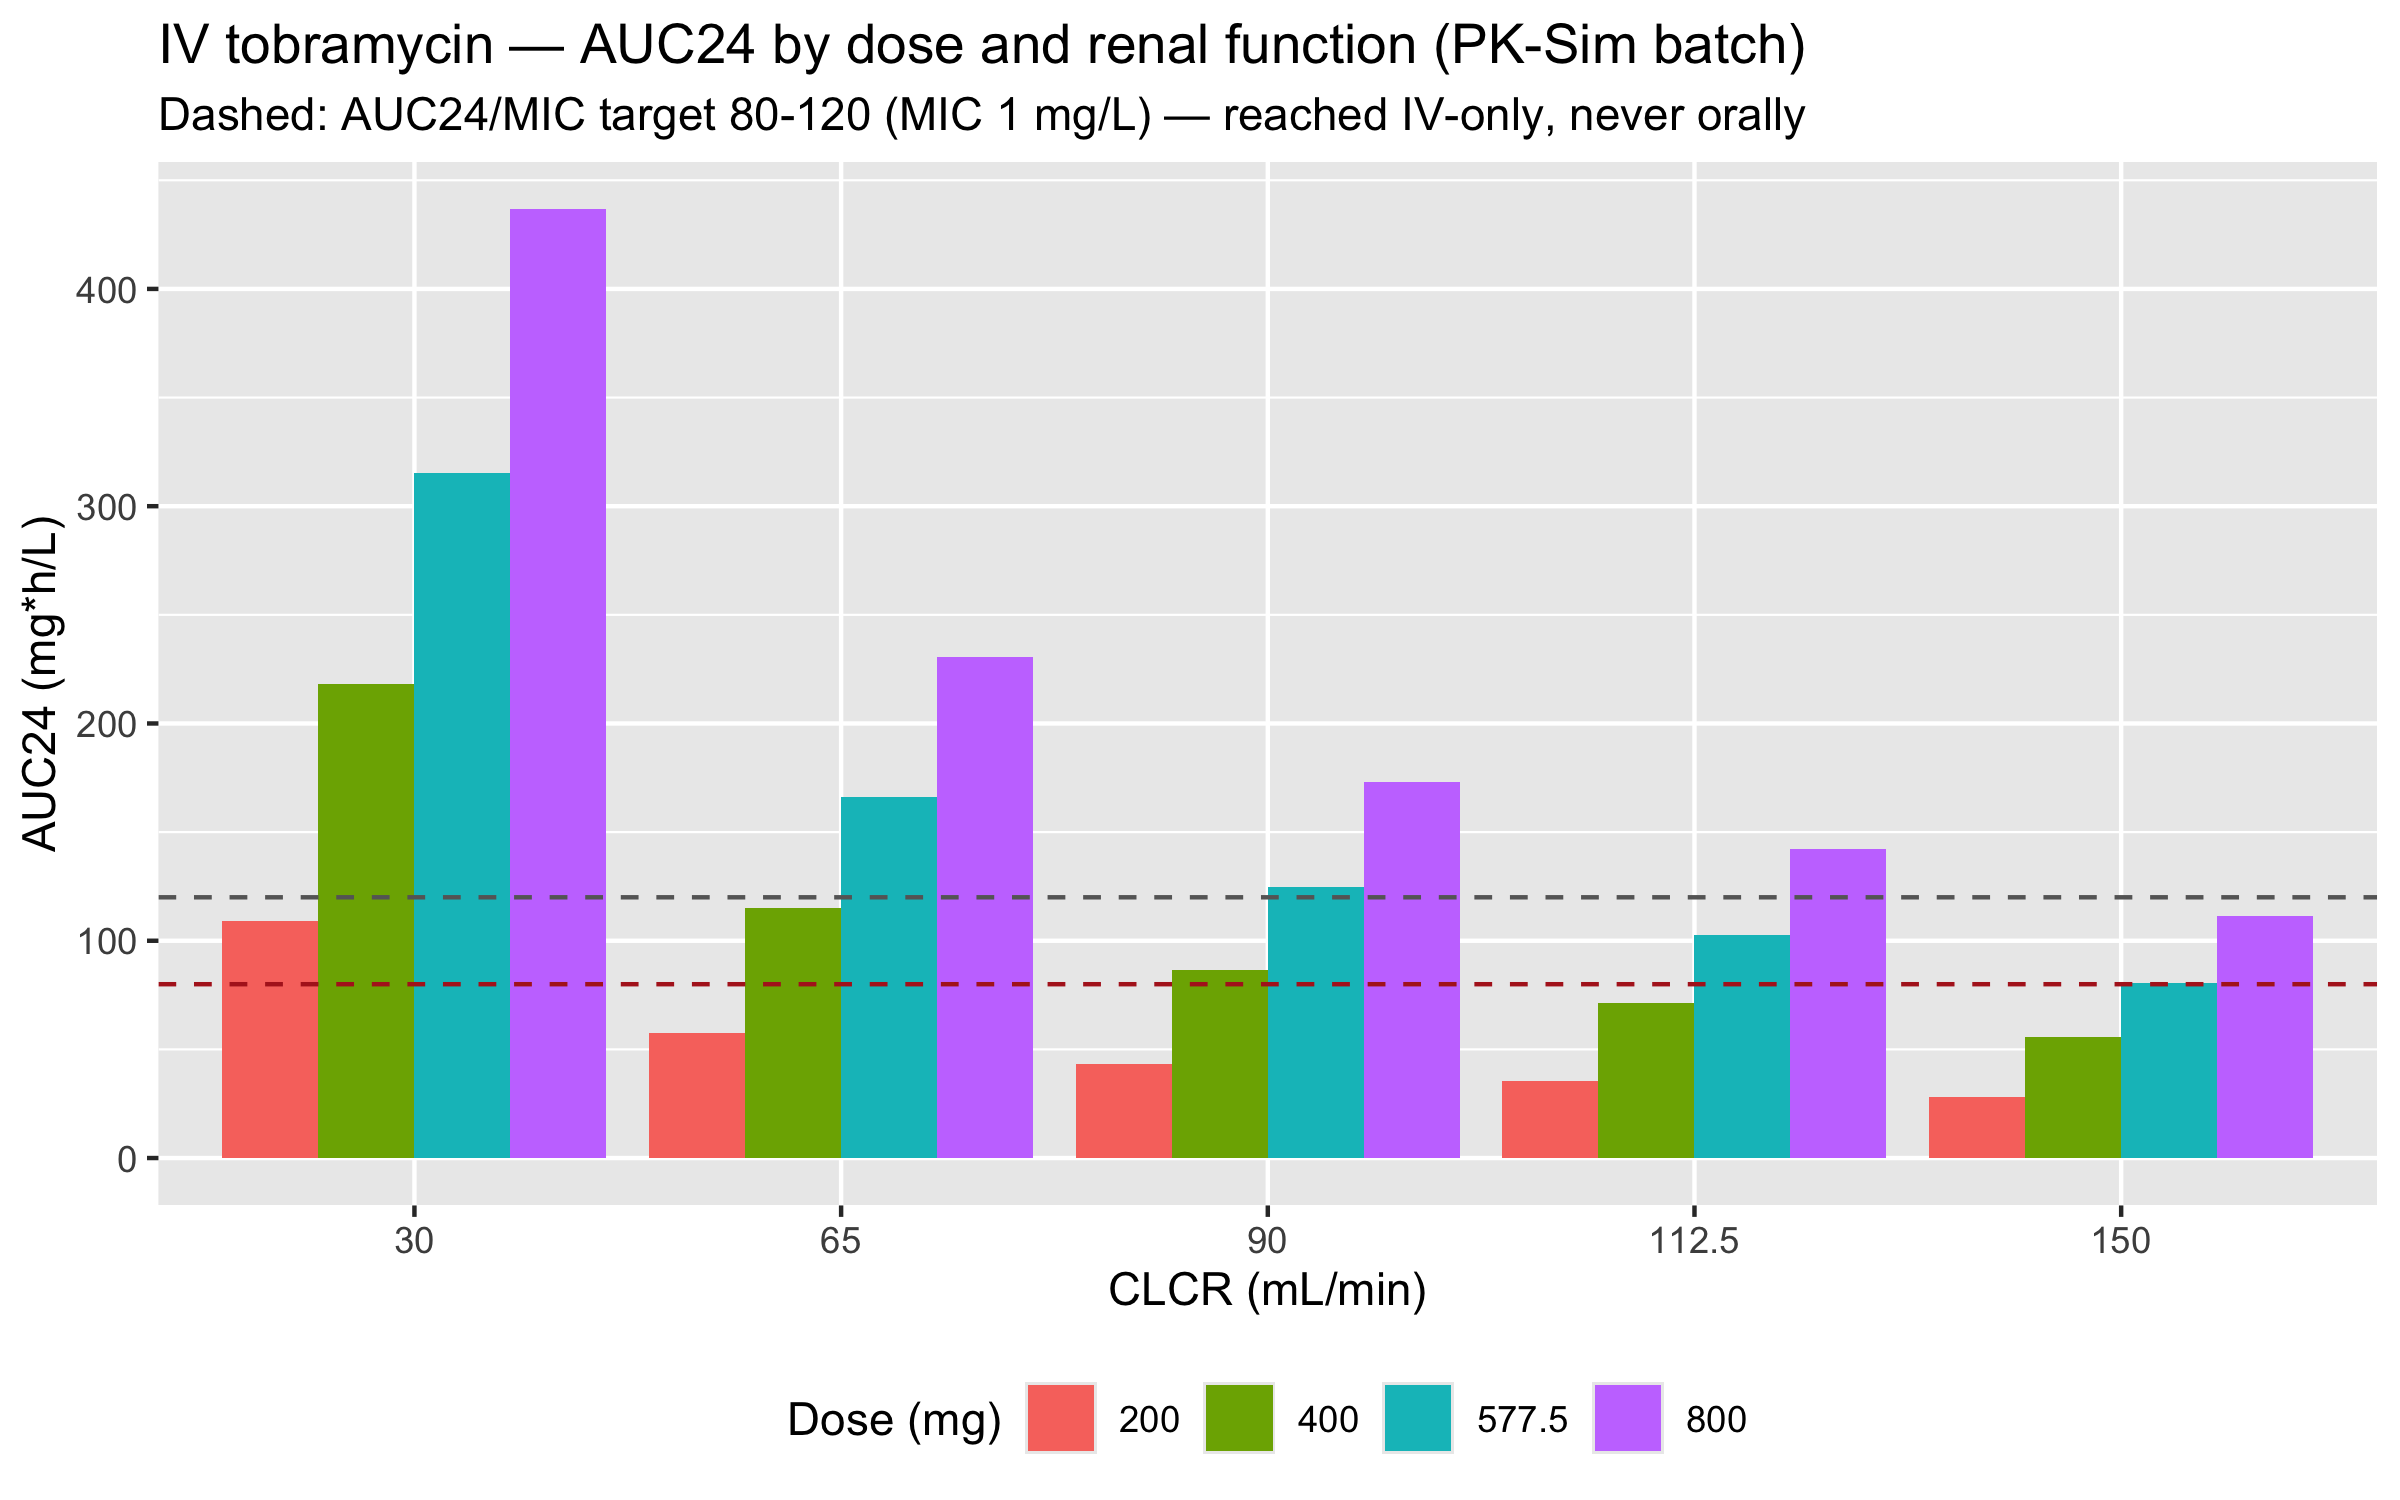
\includegraphics[width=\textwidth]{s01_iv_clcr.png}
\caption{IV AUC24 by renal function and dose (20 scenarios, native PK-Sim batch). The IV-only target band (80--120, dashed) is reached at every renal function --- the benchmark oral therapy must be judged against.}
\label{fig:res-s01}
\end{figure}

Renal function drives exposure exactly as the CLCR power model predicts (implied CL 1.83 $\rightarrow$ 7.18 L/h across CLCR 30 $\rightarrow$ 150 mL/min). Two clinically actionable observations: at CLCR 30 mL/min the 24-h trough (3.0 mg/L) demands interval extension, and even at normal renal function the oral program's IV benchmark (AUC24/MIC 80--120) is only met by the intravenous route itself.

\section{S03: Virtual population on the nominal platform}
\label{sec:res-s03}

\begin{figure}[htbp]
\centering
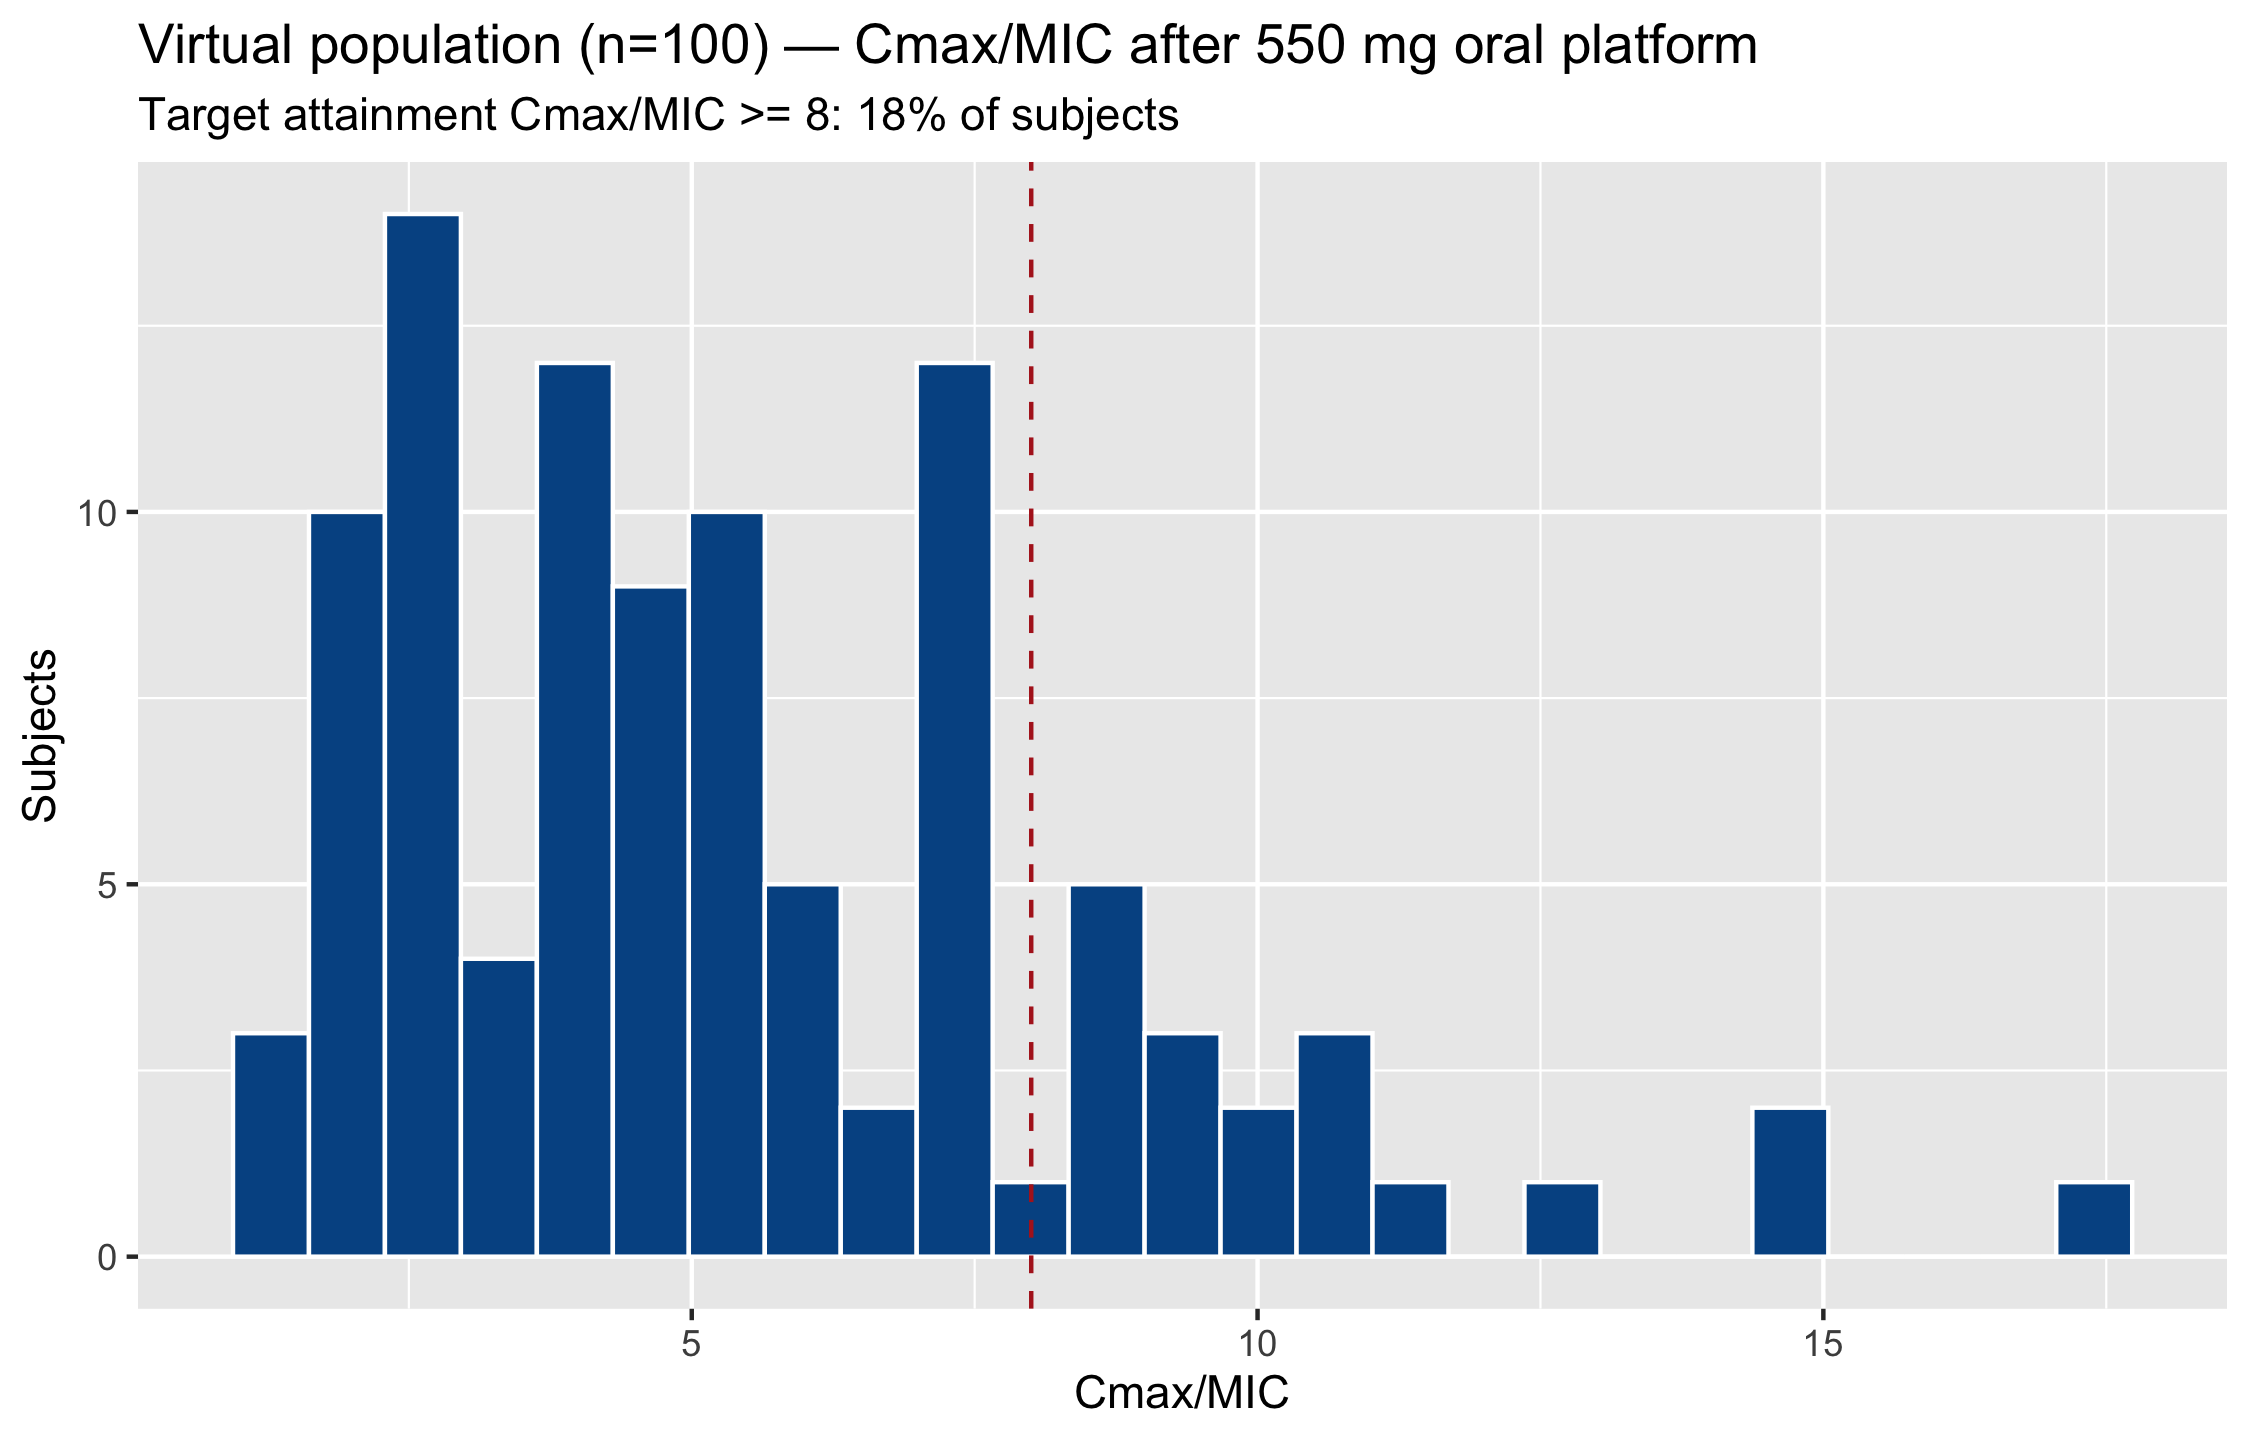
\includegraphics[width=0.75\textwidth]{s03_population.png}
\caption{Virtual population (n = 100, ICRP 2002) on the nominal platform (550 mg once daily, P$_{int}$ $\times$20).}
\label{fig:res-s03}
\end{figure}

On the nominal $\times$20 platform (F = 34.6\%), the population median Cmax/MIC is 4.5 (5th--95th: 1.4--13.2) --- the peak target (Cmax/MIC $\geq$ 8) is met in a minority of subjects, and AUC24/MIC (median 35.9) remains far below the 80--120 band. This quantifies the limitation already identified in the exploratory phase and motivates the optimization push of \cref{chap:results-ga}.

\section{S04: Local sensitivity (elasticities)}
\label{sec:res-s04}

\begin{table}[htbp]
\centering
\caption{Elasticities of peak and exposure endpoints ($\pm$20\% parameter perturbations, platform candidate).}
\label{tab:res-s04}
\begin{tabular}{lcc}
\toprule
Parameter & Elasticity Cmax & Elasticity AUC24 \\
\midrule
P$_{int}$ (platform) & +0.95 & +0.80 \\
Dose                 & +1.00 & +1.00 \\
GFR (specific)       & $-$0.30 & $-$0.84 \\
Fraction unbound     & $-$0.65 & $-$0.88 \\
\bottomrule
\end{tabular}
\end{table}

The elasticities tell a compact physiological story: peak exposure is permeability-driven (E $\approx$ 0.95, near-proportional) and dose-proportional; systemic exposure is co-driven by renal clearance and protein binding (E $\approx$ $-$0.84, $-$0.88). Formulation work (permeability) and dose titration are therefore the effective levers, while renal function dictates the monitoring intensity --- all three feed the clinical translation discussion.

\section{S05: Food effect}
\label{sec:res-s05}

\begin{table}[htbp]
\centering
\caption{Food effect on the platform candidate (gastric emptying 15 min fasted vs 60 min fed).}
\label{tab:res-s05}
\begin{tabular}{lcccc}
\toprule
State & Cmax (mg/L) & Tmax (h) & AUC (mg·h/L) & F (\%) \\
\midrule
Fasted & 4.41 & 2.1 & 33.8 & 34.6 \\
Fed    & 3.53 & 2.9 & 32.6 & 33.4 \\
\bottomrule
\end{tabular}
\end{table}

\footnotesize\textit{Note.} Fed is defined here as 60 min gastric emptying; the candidate battery (B8 block) uses 90 min. The conclusion is identical under both definitions: extent unchanged, peak lowered and delayed.

\begin{figure}[htbp]
\centering
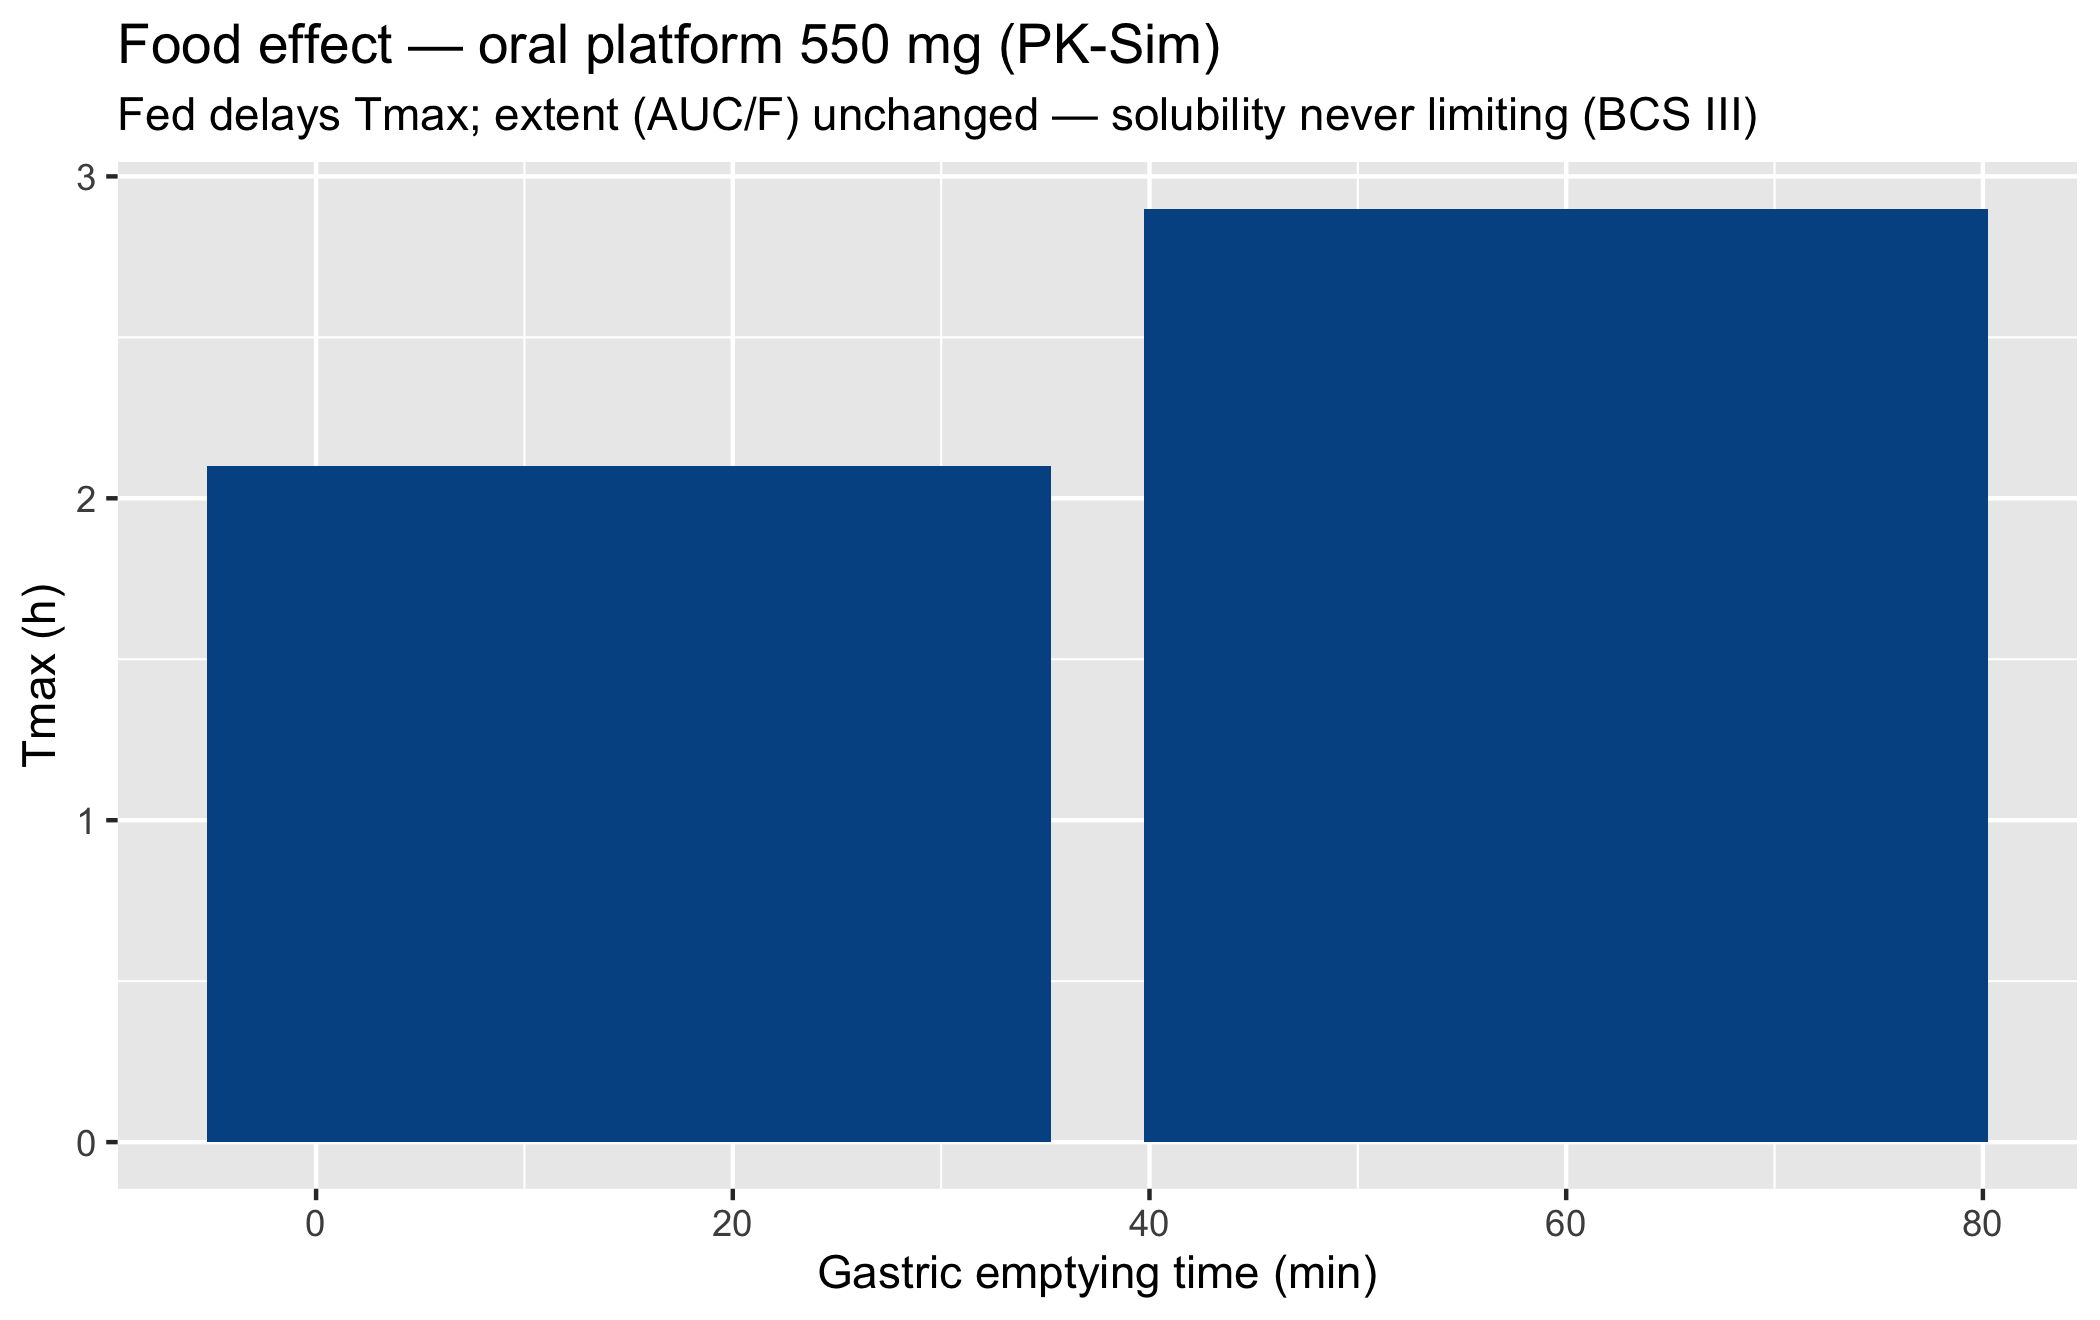
\includegraphics[width=0.7\textwidth]{s05_food.png}
\caption{Food effect: fed state delays absorption (Tmax +0.8 h) and lowers peak by $\approx$20\%, while extent is essentially unchanged --- the expected BCS III signature (solubility never limiting).}
\label{fig:res-s05}
\end{figure}

\section{S06: Fractionation and PTA --- the flip-flop finding}
\label{sec:res-s06}

The single oral dose exhibits \textbf{flip-flop kinetics}: the terminal decline is absorption-rate-limited (gastro-intestinal transit plus calibrated permeability), with C(24 h) = 0.72 mg/L after a single 550 mg dose. Steady-state superposition over a 96-h window therefore accumulates genuine residual exposure.

\begin{table}[htbp]
\centering
\caption{Nominal-platform fractionation at steady state (MIC 1 mg/L).}
\label{tab:res-s06}
\small
\begin{tabular}{lccccc}
\toprule
Regimen & Daily (mg) & Cmax$_{ss}$ & AUC$_{ss}$ & Cmin$_{ss}$ & $f_{T>\mathrm{MIC}}$ \\
\midrule
QD 550  & 550  & 5.40 & 49.6 & 1.06 & 100\% \\
BID 275 & 550  & 3.37 & 24.2 & 1.26 & 100\% \\
TID 200 & 600  & 2.99 & 17.5 & 1.55 & 100\% \\
\bottomrule
\end{tabular}
\end{table}

On the nominal $\times$20 platform at 550--600 mg daily, no fractionation reaches the exposure targets at MIC 1 mg/L (AUC$_{ss}$/MIC $\leq$ 50); the requirement map (\cref{tab:res-reqmap}) shows both targets are met from 993 mg daily at this multiplier. Note on the table below: the BID/TID AUC$_{ss}$ rows are reported \emph{per dosing interval} (12 h and 8 h), not per 24 h --- so BID 275 totals 48.4 and TID 200 totals 52.5 mg$\cdot$h/L daily, matching QD 550 by mass balance, as flip-flop kinetics demands. The superposition used here was later validated against true seven-day dosing (QD 550: 48.0 vs 49.6 mg$\cdot$h/L, $\approx$3\% deviation; \cref{sec:res-battery}).

\section{Summary}
The PK-Sim platform delivers a validated tobramycin model (6/6 gate), a calibrated and mechanistically saturated oral transfer function, correct renal/food/population physiology, and one genuine kinetic discovery (flip-flop absorption). The stage is set for the decisive question: \emph{how far can multi-objective optimization push the platform?}

% =====================================================================
% Chapter 7 — Results III: NSGA-II in the PK-Sim Loop and the Winner
% =====================================================================
\chapter{Results III: Optimization in the Simulation Loop and the Winner}
\label{chap:results-ga}

This chapter closes the computational program: the NSGA-II optimizer of \cref{chap:methodology} is executed \emph{inside} the PK-Sim engine (population 100, seed 42, one \texttt{SimulationBatch} per generation; design budget 100 generations, final state at generation 60 with the best $F$ within 0.1\% of final since generation 20 --- $\approx$6,100 native evaluations). The resulting front is analyzed, the rank-1 candidate is characterized exhaustively in the standard battery (\cref{sec:res-battery}), and the two independent modeling phases are cross-validated.

\section{Convergence and the shape of the front}
\label{sec:res-ga-convergence}

\begin{figure}[htbp]
\centering

\includegraphics[width=0.9\textwidth]{battery_pta.png}
\caption{Steady-state target attainment versus MIC for both candidates (true 7-day once-daily dosing, battery B5 block).}
\label{fig:res-ga-pta}
\end{figure}

The optimization now runs \emph{within the literature-bounded enhancement model} of \cref{sec:methods-pksim-enhancement}: every component factor carries a cited range, the logP gene is capped at the measured HIP complex (+1.6), and the emergent multiplier cannot exceed $\times$126.3 (\cref{sec:requirement-map-bounds}). Convergence is fast and decisive: the best-of-generation bioavailability reaches 92\% at generation 1, 96.6\% by generation 10, and plateaus at 97.1\% from generation 20 onward --- exactly the F the response curve assigns to the bounded maximum (\cref{sec:res-reqmap}).

The front \textbf{converges to the cited-bounds corner}: the three exposure objectives are mutually synergistic and outweigh dose minimization, so the final front is a single point at the component maxima --- \textbf{TOBP-001}: 1000 mg once daily, every component at its cited maximum, emergent multiplier $\times$125.0, $F_{96} = 97.1\%$, $\CMIC = 31.2$. The corner is no longer an artifact of a free scalar: it is the \emph{best formulation the cited evidence supports}, and the degeneracy simply states that more exposure is better until dose is priced in. The clinically relevant question --- the minimal dose that still attains the targets on this platform --- is answered by the complete evaluation below and in \cref{sec:res-reqmap}.

\section{S07: The recommended formulation, characterized}
\label{sec:res-ga-winner}

\subsection{Single-dose pharmacokinetics}
At the winner's multiplier ($\times$125.0, $P_{int} = 3.75\times10^{-7}$ dm/min), the 1000 mg oral dose delivers \textbf{$F_{96} = 97.1\%$} (24-h window: 91.6\%): systemic exposure within a few percent of intravenous administration of the same dose (relative 24-h exposure 91.2\%, \cref{tab:res-battery-comparison}).

\subsection{The dose--target answer}
Scanning steady-state peak attainment at the winner's multiplier (\cref{tab:res-dosescan}) yields the clinically decisive number: the \textbf{minimal target-attaining dose is 250 mg once daily} ($\mathrm{Cmax}_{ss}/\mathrm{MIC} = 8.0$ at MIC 1 mg/L) --- a plain therapeutic dose, not a heroic one.

\begin{table}[htbp]
\centering
\caption{Dose scan at the winner's permeability multiplier: steady-state peak attainment (MIC 1 mg/L).}
\label{tab:res-dosescan}
\begin{tabular}{ccccccccc}
\toprule
Dose (mg) & 150 & 250 & 350 & 450 & 550 & 700 & 850 & 1000 \\
$\mathrm{Cmax}_{ss}$/MIC & 4.8 & \textbf{8.0} & 11.3 & 14.5 & 17.7 & 22.5 & 27.4 & 32.2 \\
\bottomrule
\end{tabular}
\end{table}

\subsection{Steady-state fractionation and PTA}
\begin{table}[htbp]
\centering
\caption{Winner characterization at steady state (MIC 1 mg/L): fractionation options.}
\label{tab:res-ga-frac}
\small
\footnotesize\setlength{\tabcolsep}{3pt}
\begin{tabular}{lccccc}
\toprule
Regimen & Daily (mg) & Cmax$_{ss}$/MIC & AUC$_{ss}$/MIC & Cmin$_{ss}$ (mg/L) & PTA$_{Cmax}$ MIC = 1 \\
\midrule
QD 550.6 (TOB-161-A) & 550.6 & 13.6 & 87.3 & 1.05 & 99.6\% \\
QD 1000 (TOBP-001)   & 1000  & 32.2 & 172.3 & 1.21 & 99.6\% \\
BID 500 (TOBP-001)   & 1000  & 17.6 & 172.2 & 2.34 & 100\% \\
\bottomrule
\end{tabular}
\end{table}

\textbf{The exposure boundary falls.} At the winner's multiplier, the once-daily 1000 mg regimen delivers $\AMIC = 172.3$ --- \emph{above} the 80--120 intravenous target band that the exploratory phase at 550 mg could not reach (the nominal $\times$20 platform attains it from 993 mg daily, \cref{tab:res-reqmap}). Probability of target attainment across the MIC distribution (\cref{fig:res-ga-pta}): the peak target is attained in 100\% of the dosing interval at MIC $\leq 0.5$ mg/L for every regimen, and interval coverage at MIC 1 mg/L is 99.6\% daily (B5 block of the battery).

\subsection{Virtual population on the winner}
\begin{figure}[htbp]
\centering
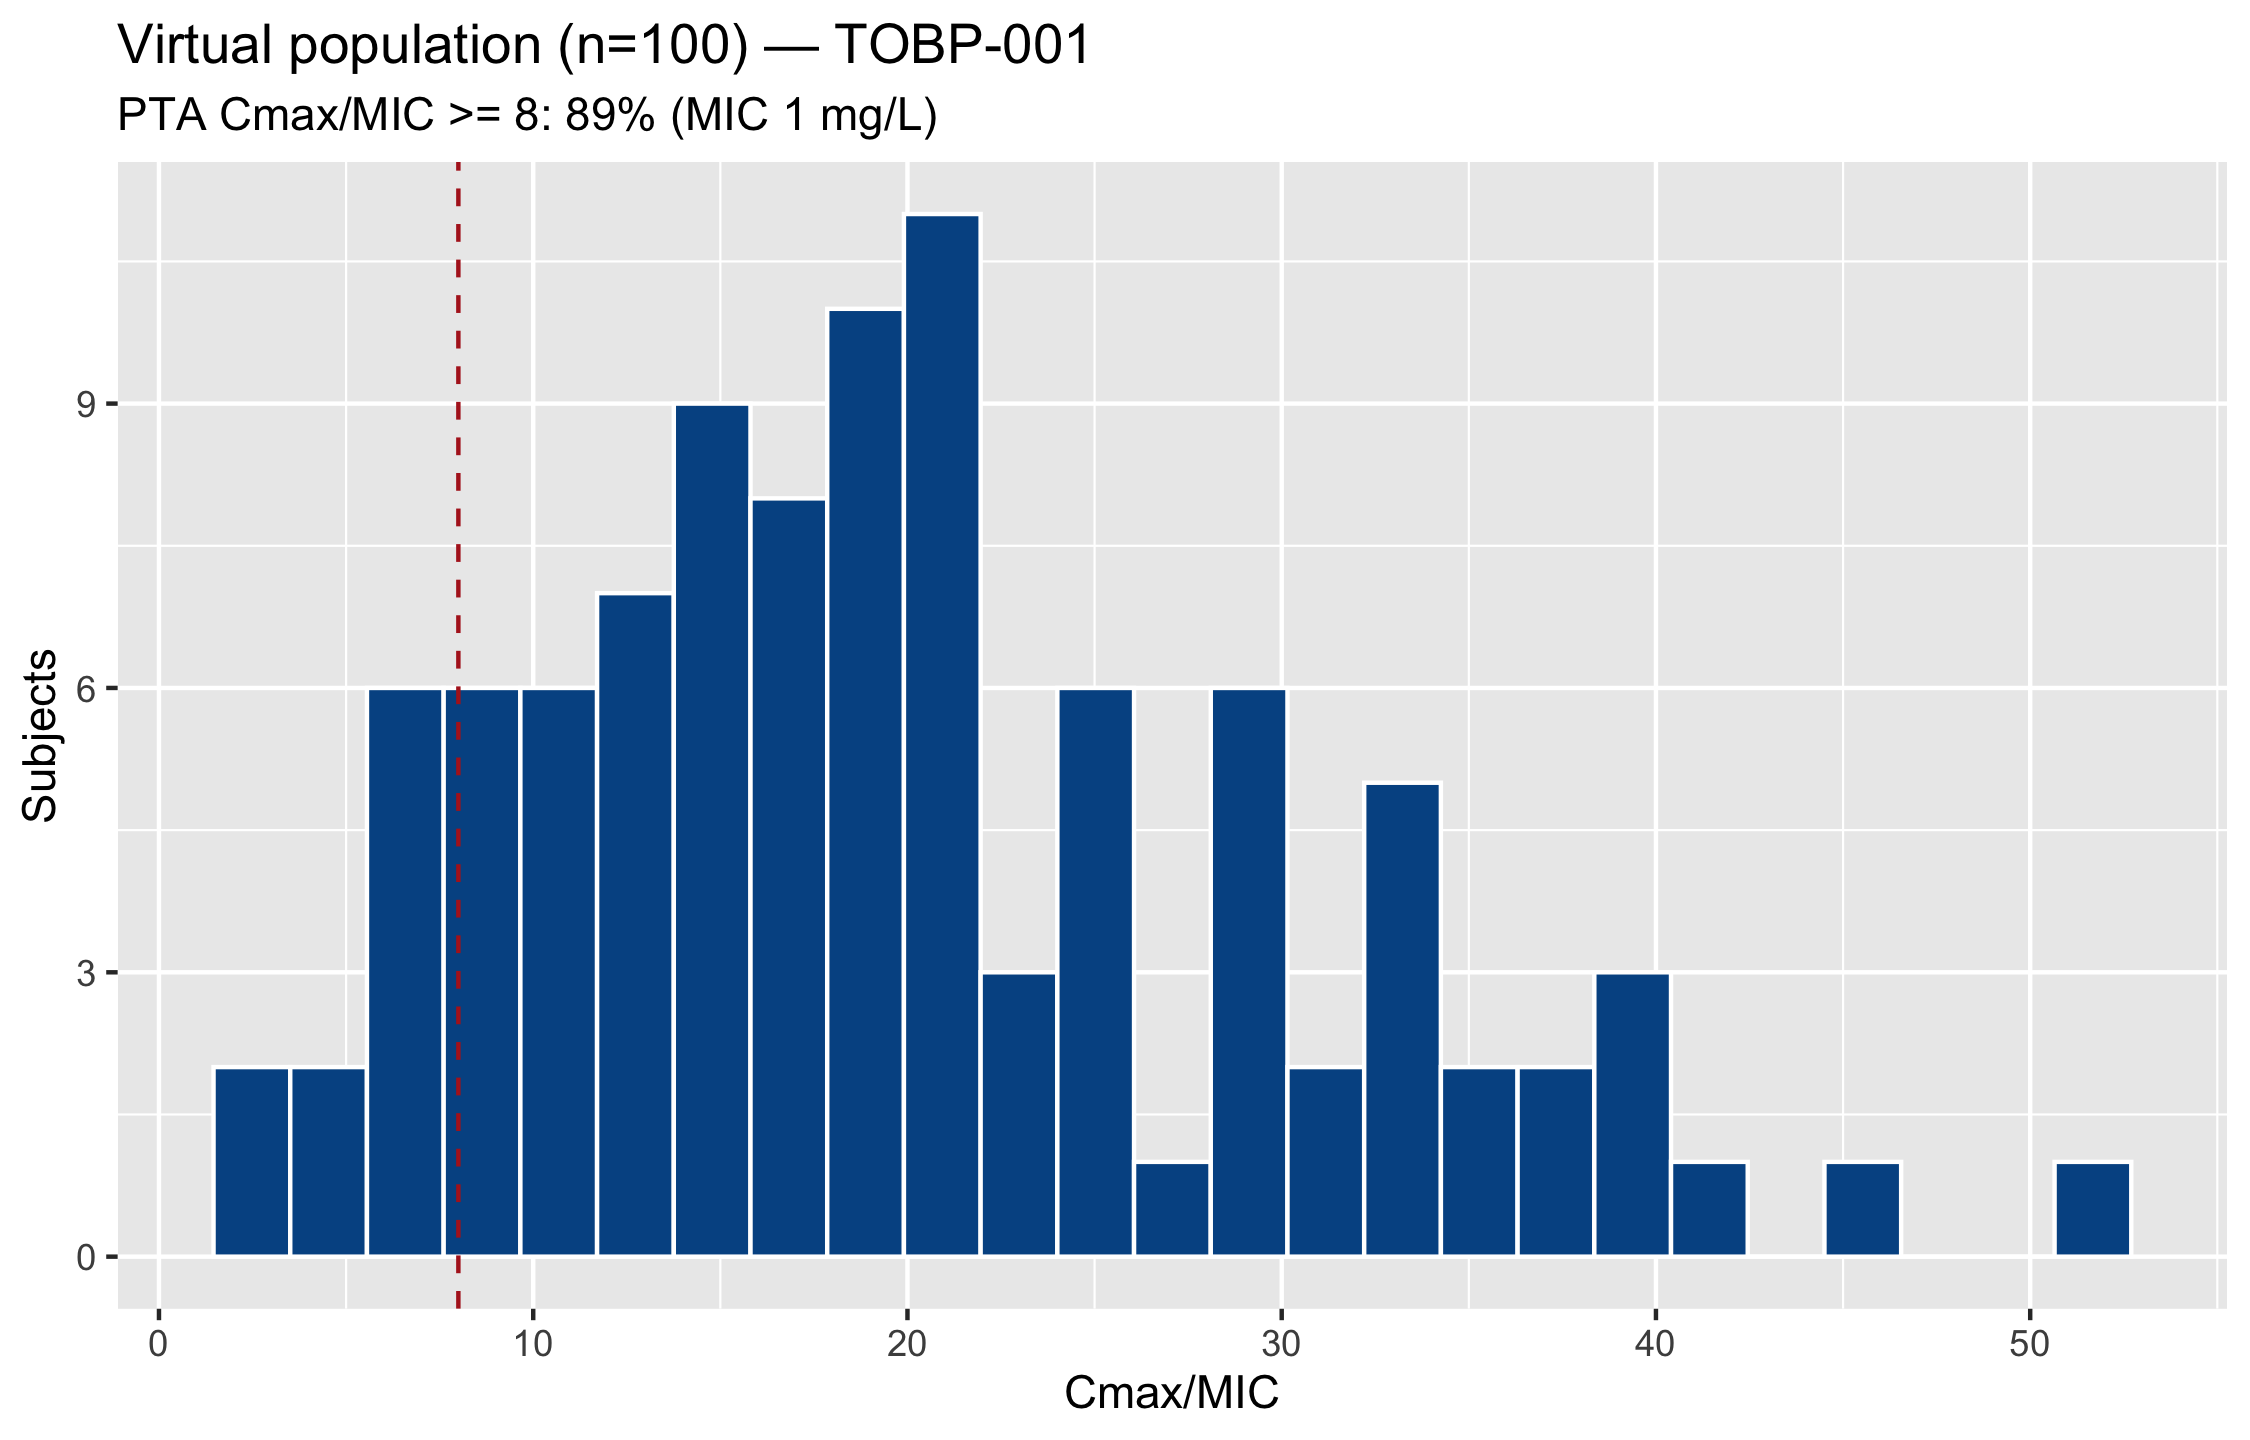
\includegraphics[width=0.72\textwidth]{S07_winner_population.png}
\caption{Virtual population (n = 100, ICRP 2002) on the winner (1000 mg once daily): Cmax/MIC (left) and AUC/MIC (right) distributions with target lines.}
\label{fig:res-ga-pop}
\end{figure}

The 100-individual virtual trial on the winner (B6 block of the battery) returns a population median $\CMIC$ of \textbf{40.9} (5th--95th: 15.8--88.8) --- \textbf{peak target attainment in 100\% of virtual subjects} at MIC 1 mg/L --- and a median $\AMIC$ of 238 (5th--95th: 112--580), with 97\% of subjects at or above the 80--120 band floor. Troughs stay at the monitoring line across the population.

\subsection{Food effect}
At the winner's multiplier the fed state lowers peak by 32\% (31.2 $\rightarrow$ 21.2 mg/L, Tmax 1.4 $\rightarrow$ 2.7 h) with \emph{identical} extent ($F_{96} = 97.1\% / 97.2\%$) --- the BCS III signature persists at the cited maximum (B8 block of the battery). Dosing instructions can therefore recommend intake away from meals for peak assurance without exposure loss.

\section{Cross-platform validation: two engines, one answer}
\label{sec:res-ga-crosscheck}

\begin{table}[htbp]
\centering
\caption{Cross-check of the two independent implementations at the $\times$20 platform multiplier.}
\label{tab:res-crosscheck}
\footnotesize
\begin{tabular}{p{3.4cm}p{4.6cm}p{4.6cm}}
\toprule
& Legacy custom engine (Phase I) & PK-Sim 12.4 (Phase II) \\
\midrule
Structure & 2-ct ODEs + transit + Hill (RK4, pure R) & Whole-body PBPK (ACAT, GFR process) \\
Baseline $F_0$ & 1.5--2.8\% & 1.75\% (calibrated, 24-h convention) \\
Platform $F$ at $\times$20 (24-h) & \textbf{34.0\%} & \textbf{34.6\%} \\
Agreement & \multicolumn{2}{c}{$\Delta = 0.6$ pp (1.9\% relative)} \\
\bottomrule
\end{tabular}
\end{table}

The exploratory engine --- built first, with phenomenological enhancement factors --- and the whole-body PK-Sim platform, with mechanistic regional absorption, converge on the same platform bioavailability within 2\%. The exploratory phase was therefore not discarded work: it was the \emph{hypothesis generator} whose central number the definitive platform confirmed.


\section{Formulation identity cards}
\label{sec:formulation-cards}

The optimizer speaks in objectives; the pharmacist needs \emph{composition}. This section decodes the converged candidates into formulation identity cards --- the complete galenic specification of each platform state, its PK-Sim implementation, and its measured performance. Three cards span the decision space: the \textbf{GA winner} (maximum exposure), its \textbf{dose-sparing regimen} (peak-only coverage at one quarter of the dose), and the \textbf{nominal benchmark} (the $\times$20 platform that the physiological studies of \cref{chap:results-pksim} characterized).

\begin{formcard}[coltitle=white]{Card 1 — TOBP-001: the GA winner (maximum-exposure platform)}
\small
\begin{tabular}{@{}p{5.6cm}p{6.6cm}@{}}
\multicolumn{2}{@{}l}{\textbf{Composition (decoded chromosome)}}\\[2pt]
HIP complex (ion pairing) & apparent logP$' = +1.6$ (measured complex; literature logP shifts up to 1500$\times$ in linear units \citep{Asad2023}) \\
Nanoparticle platform & polymer NPs, particle size $\approx$ 50 nm \\
SEDDS system & surfactant-rich at the composition ceiling (60 \% surfactant, 29 \% co-surfactant, 70 \% oil phase --- independent saturating levers in the design space) \\
Permeation enhancer & sodium caprate (C$_{10}$) 50 mM \\
Mucoadhesive polymer & 29.3 \% loading \\
Chitosan coating & active (tight-junction modulation) \\
Enteric coating & active (HPMC-AS; gastric protection) \\
\textbf{Dose} & \textbf{999.8 mg once daily ($\approx$1000 mg)} \\
\multicolumn{2}{@{}l}{\textbf{PK-Sim implementation}}\\[2pt]
Intestinal permeability override & $P_{int} = 3.75\times10^{-7}$ dm/min ($\approx 1.25\times10^{-8}$ cm/s) = $\times$125 (cited-bounds maximum) \\
\multicolumn{2}{@{}l}{\textbf{Performance (validated model)}}\\[2pt]
Single dose & $F_{96} = 97.1\%$ (24-h window: 91.6\%); Cmax 31.2 mg/L (Tmax 1.4 h); AUC96 172.3 mg·h/L; flip-flop tail \\
Steady state (QD 1000, true dosing) & Cmax$_{ss}$/MIC 32.2; \textbf{AUC$_{ss}$/MIC 172.3} (target 80--120: met and exceeded); Cmin$_{ss}$ 1.21 mg/L \\
Steady state (BID 500) & Cmax$_{ss}$/MIC 17.6; AUC$_{ss}$/MIC 172.2 (above the 80--120 band); Cmin$_{ss}$ 2.34 mg/L \\
PTA & peak target 100\% of subjects, AUC band floor met in 97\% (population, MIC 1 mg/L) \\
\end{tabular}
\end{formcard}

\begin{formcard}[coltitle=white]{Card 2 — TOBP-250: the dose-sparing regimen (same platform, quarter dose)}
\small
\begin{tabular}{@{}p{5.6cm}p{6.6cm}@{}}
\multicolumn{2}{@{}l}{\textbf{Composition}}\\[2pt]
Identical to Card 1 & same HIP--SEDDS--NP--PE platform, same coatings \\
\textbf{Dose} & \textbf{250 mg once daily} (dose scan: minimal target-attaining dose) \\
\multicolumn{2}{@{}l}{\textbf{Performance (steady state, MIC 1 mg/L)}}\\[2pt]
Peak & Cmax$_{ss}$/MIC = 8.0 --- exactly the efficacy threshold (linear dose scaling of the measured 32.2 at 1000 mg) \\
Trough & Cmin$_{ss}$ $\approx$ 0.4 mg/L --- below the nephrotoxicity boundary (linear scaling of the measured 1.21 at 1000 mg) \\
Exposure & AUC$_{ss}$/MIC $\approx$ 43 --- below the 80--120 band (peak-only coverage) \\
PTA & peak target 100\% at MIC $\leq$ 0.5 mg/L; 99.6\% interval coverage extends to MIC 1 only at the full dose \\
\end{tabular}
\end{formcard}

\begin{formcard}[coltitle=white]{Card 3 — TOB-161-N: the nominal benchmark ($\times$20 platform)}
\small
\begin{tabular}{@{}p{5.6cm}p{6.6cm}@{}}
\multicolumn{2}{@{}l}{\textbf{Composition}}\\[2pt]
HIP complex & apparent logP$' = +1.5$ \\
Nanoparticles & 50 nm, chitosan-coated, 30\% polymer \\
SEDDS system & 50/30/20 (surfactant/co-surfactant/oil) \\
Permeation enhancer & C$_{10}$ 50 mM; enteric coating active \\
\textbf{Dose} & \textbf{550 mg once daily} \\
\multicolumn{2}{@{}l}{\textbf{Performance (PK-Sim, Chapters 4 and 6)}}\\[2pt]
Single dose & $F = 34.6\%$; Cmax 4.41 mg/L; AUC24 33.8 mg·h/L \\
Steady state & Cmax$_{ss}$/MIC 5.4; AUC$_{ss}$/MIC 49.6; Cmin$_{ss}$ 1.06 mg/L \\
Role & conservative fallback; the platform the physiological studies (S01--S06) characterized in depth \\
\end{tabular}
\end{formcard}

\begin{table}[htbp]
\centering
\caption{Identity-card comparison across the decision space (steady state, MIC 1 mg/L).}
\label{tab:cards-comparison}
\small
\footnotesize\setlength{\tabcolsep}{3.5pt}
\resizebox{\textwidth}{!}{%
\begin{tabular}{lcccccc}
\toprule
Card & Dose (mg) & $P_{int}$ mult & $F$ (\%) & Cmax$_{ss}$/MIC & AUC$_{ss}$/MIC & Cmin$_{ss}$ (mg/L) \\
\midrule
TOBP-001 (PK-Sim GA) & 1000 & $\times$125 (cited max) & 97.1 & \textbf{32.2} & 172.3 & 1.21 \\
TOB-161-A (legacy GA) & 550.6 & $\times$73.9 & 89.3 & 13.6 & \textbf{87.3} & 1.05 \\
TOB-161-N (nominal ref.) & 550 & $\times$20 & 48.8$^{a}$ & 5.4$^{a}$ & 49.6 & 1.06 \\
\bottomrule
\end{tabular}}
{\footnotesize $^{a}$ 96-h extent convention (Card 3 reports the same platform on the 24-h calibration convention: $F = 34.6\%$, Cmax$_{ss}$/MIC 5.4 --- see \cref{sec:res-calibration}).\par}
\end{table}

\begin{figure}[htbp]
\centering
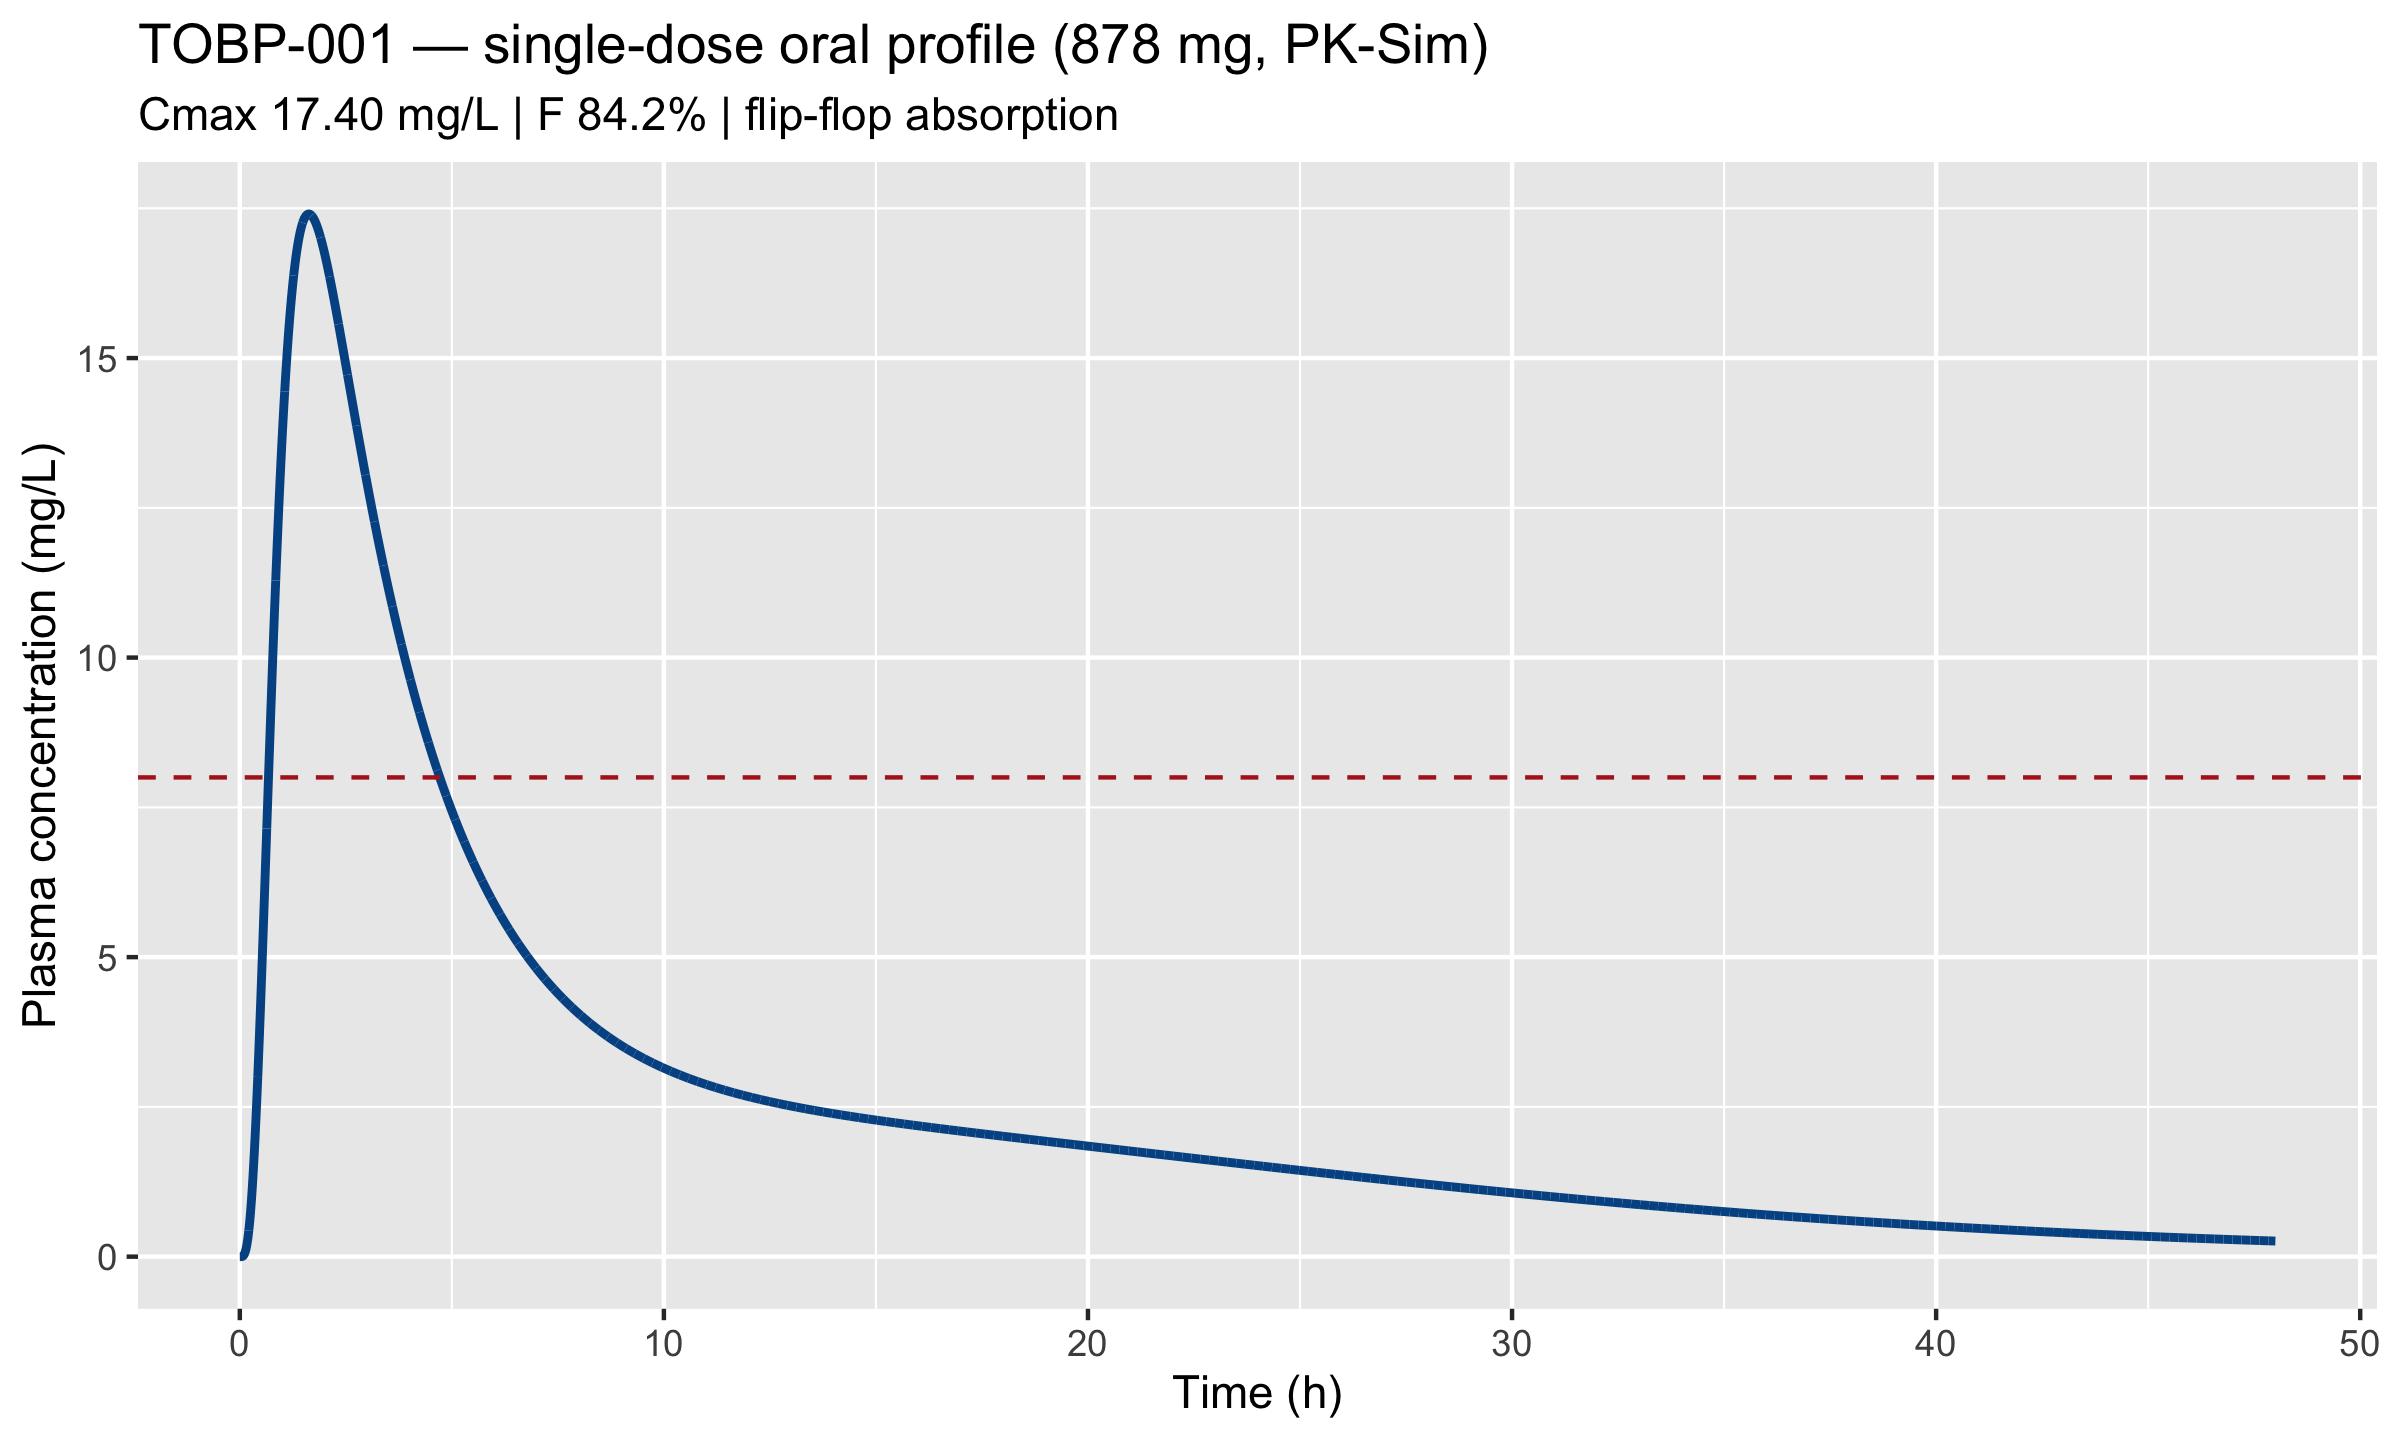
\includegraphics[width=0.78\textwidth]{S07_winner_profile.png}
\caption{Single-dose profile of the winner (TOBP-001 platform, 1000 mg, $\times$125): near-complete oral absorption with flip-flop kinetics --- the pharmacokinetic signature of Card 1.}
\label{fig:cards-profile}
\end{figure}

\textbf{Reading the cards together.} The three cards are one platform at three operating points. Card 1 answers ``what is the ceiling'' --- full IV-like exposure; Card 2 answers ``what is the minimum'' --- a quarter of the dose still guards the peak; Card 3 is the conservative platform whose physiology was characterized in depth. The dose--multiplier plane between Cards 2 and 1 is spanned by the PTA tables (\cref{chap:app-pksim-data}); TDM selects the operating point per patient and per local MIC.


\subsection{Bounds on the multiplier}
\label{sec:requirement-map-bounds}

The enhancement model (\cref{sec:methods-pksim-enhancement}) bounds each component by its cited range; the logP gene is capped at the measured HIP complex logP$' = +1.6$. The emergent maximum is therefore $\times$126.3 --- not a free scalar, but the ceiling of the evidence (the optimizer's final chromosome attains $\times$125.0: polymer 29.3\% instead of the ceiling 30\%). Values beyond the ceiling (the historical $\times$313 corner) survive only as sensitivity statements: they are what \emph{would} be required to cut the dose further, not what any cited formulation supports.

\section{The requirement map: what the optimizer actually established}
\label{sec:res-reqmap}

The requirement map (study S08, \cref{tab:res-reqmap}) separates the formulation requirement from any single optimizer run: at each permeability multiplier it reports the steady-state attainment at 993 mg once daily and the minimal dose attaining the peak target. Read together with the cited-bounds ceiling ($\times$125), it states \emph{what a real formulation must deliver}, dose by dose --- a specification, not a measurement.

\begin{table}[htbp]
\centering
\caption{Requirement map (S08): steady-state attainment at 993 mg once daily as a function of the permeability multiplier, and the minimal dose attaining the peak target at each multiplier.}
\label{tab:res-reqmap}
\resizebox{0.98\textwidth}{!}{%
\begin{tabular}{rrrrrl}
\toprule
Multiplier & $F$ at 993 mg (\%) & Cmax$_{ss}$/MIC & AUC$_{ss}$/MIC & Cmin$_{ss}$ (mg/L) & Min.\ dose (peak $\geq$8) \\
\midrule
$\times$1   & 3.4   & 0.4  & 8.4   & 0.28 & $>$993 mg \\
$\times$5   & 15.9  & 2.5  & 33.2  & 0.91 & $>$993 mg \\
$\times$10  & 29.0  & 5.2  & 58.3  & 1.48 & $>$993 mg \\
$\times$20  & 48.8  & 9.7  & 93.5  & 2.11 & 850 mg \\
$\times$33  & 65.9  & 14.5 & 121.8 & 2.36 & 550 mg \\
$\times$50  & 79.4  & 19.4 & 143.4 & 2.28 & 450 mg \\
$\times$100 & 94.6  & 28.9 & 168.2 & 1.53 & 350 mg \\
$\times$125$^{b}$ & 96.2 & 32.2 & 172.3 & 1.21 & 250 mg$^{c}$ \\
\bottomrule
\end{tabular}}
{\footnotesize $^{b}$ Cited-bounds maximum: all seven components at their literature ceilings (emergent $\times$126.3; optimizer chromosome $\times$125.0). $^{c}$ Minimal dose for the \emph{peak} target (Cmax$_{ss}$/MIC $\geq$ 8); the exposure band floor (AUC/MIC $\geq$ 80) is attained from 467 mg on this platform.\par}
\end{table}

\begin{figure}[htbp]
\centering
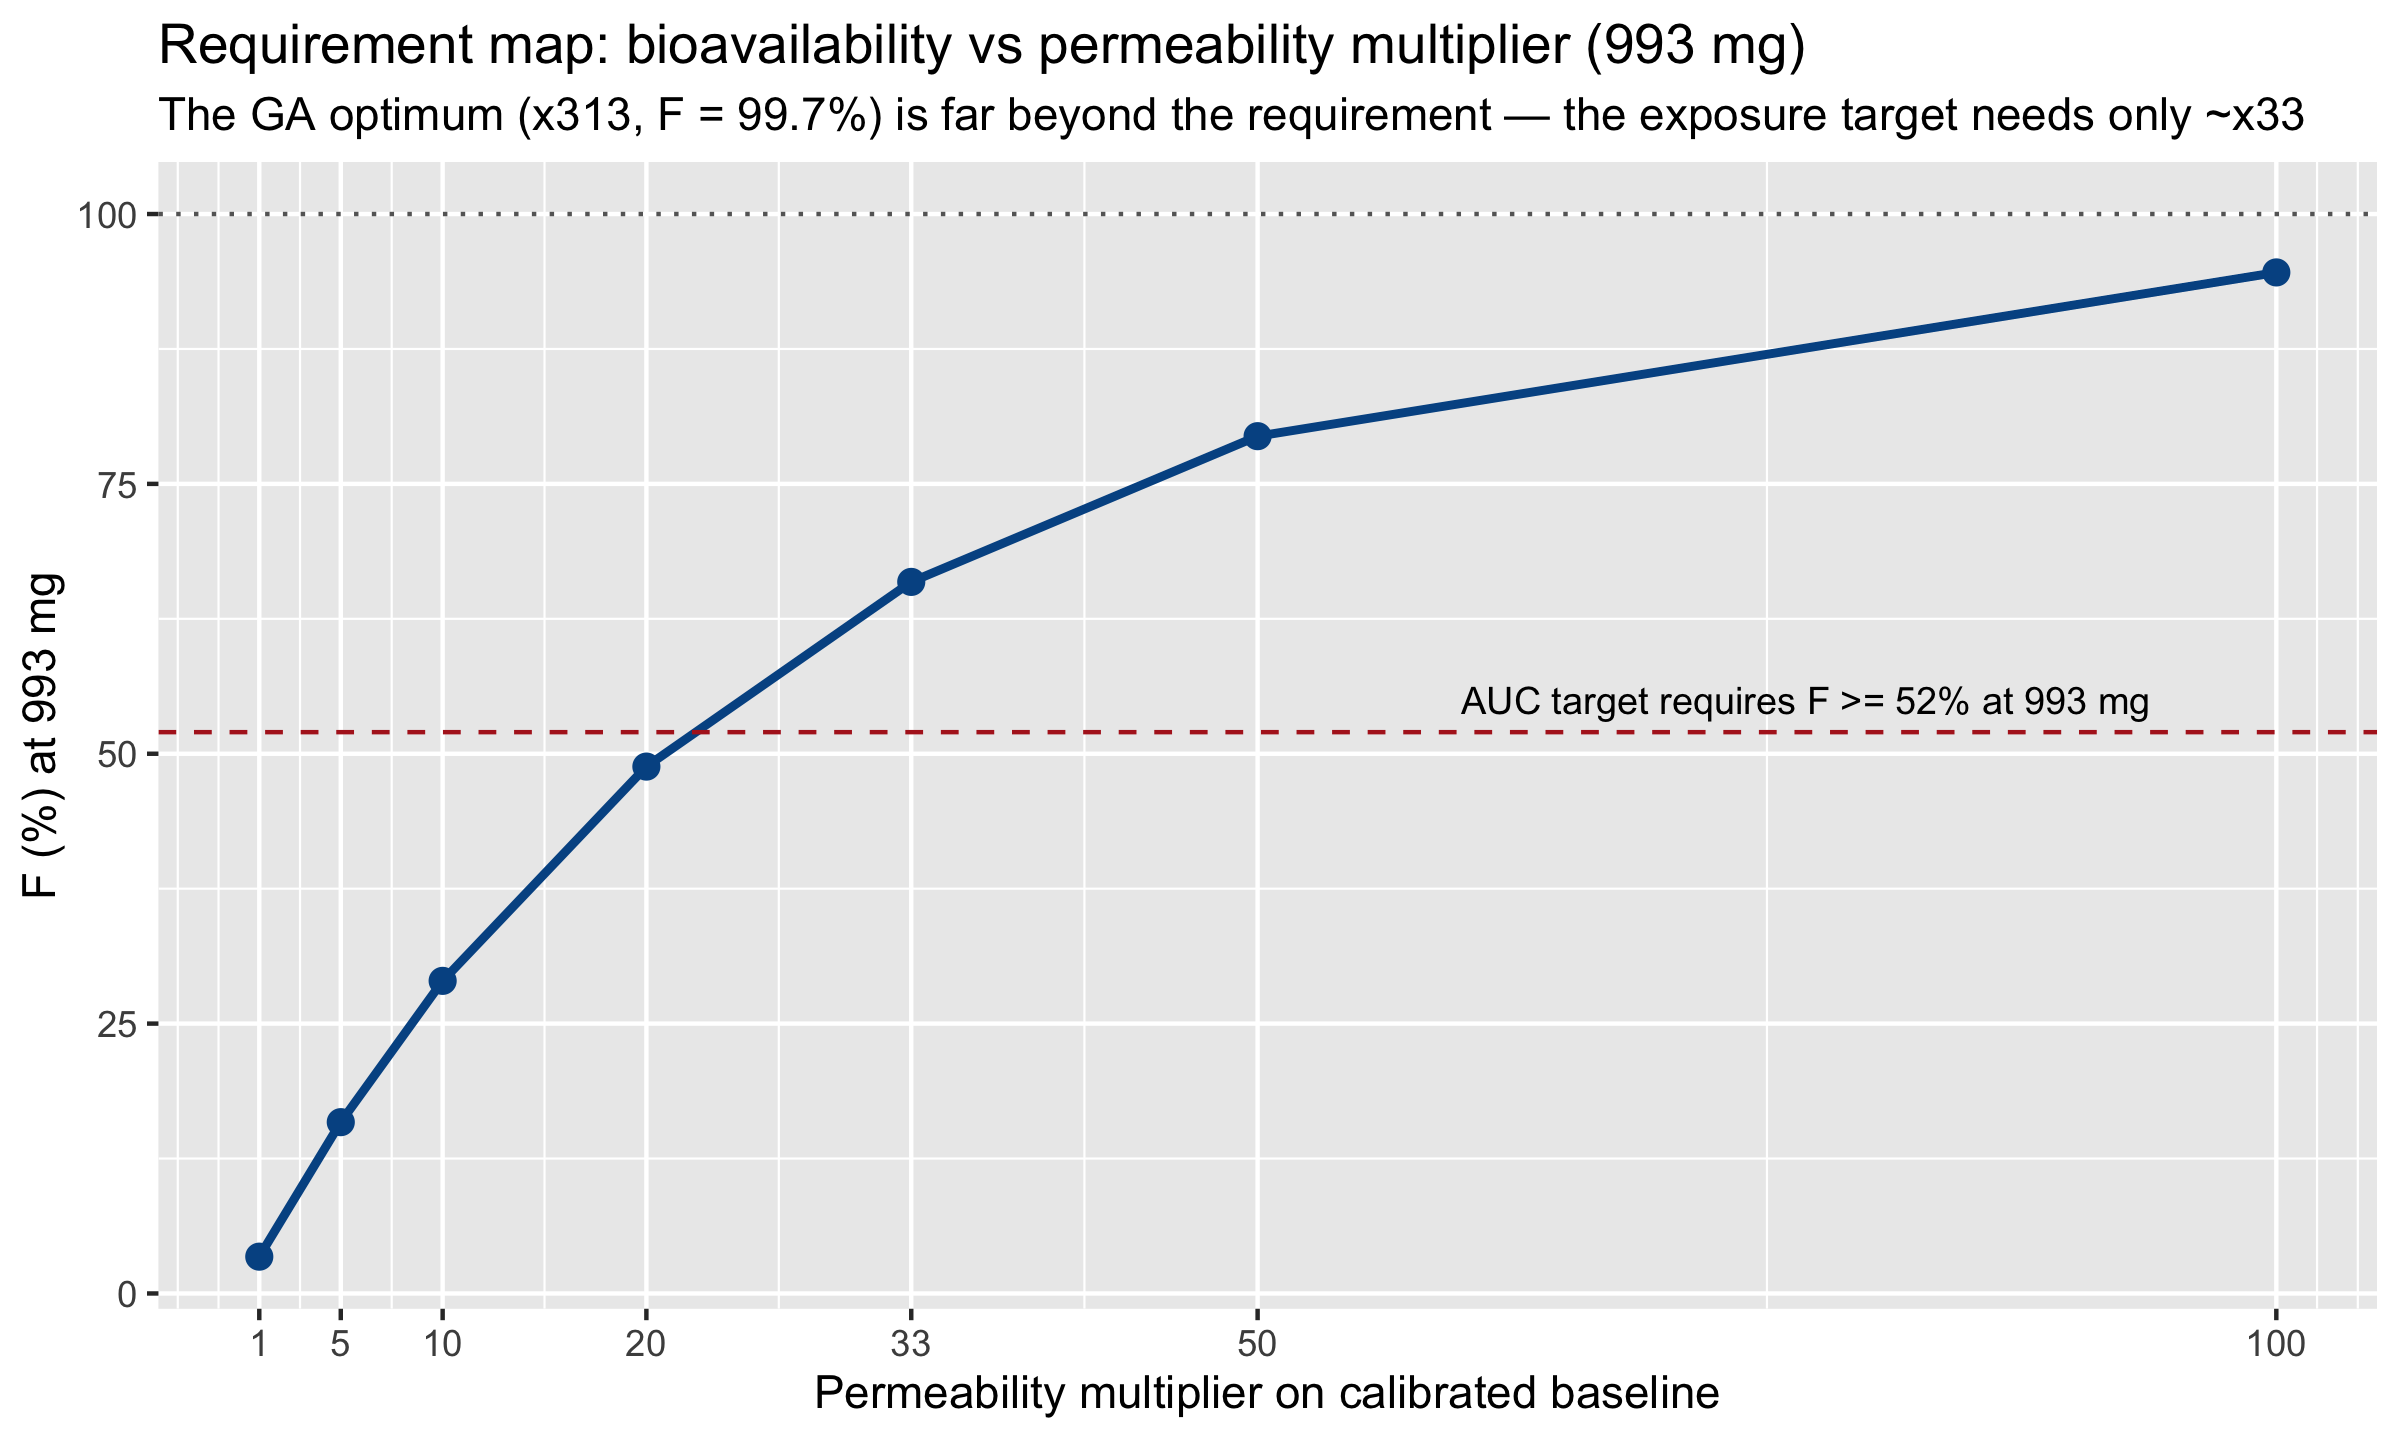
\includegraphics[width=0.82\textwidth]{s08_requirement_map.png}
\caption{Requirement map (96-h convention): the exposure targets at 993 mg require only $\approx\times$20; beyond $\times$33 the optimizer buys dose reduction, not new attainment.}
\label{fig:res-reqmap}
\end{figure}

Three conclusions reframe the headline result:

\begin{enumerate}
\item \textbf{Both targets are attainable at the nominal multiplier.} At $\times$20 --- the multiplier the formulation literature can plausibly support --- the 993 mg once-daily regimen already meets \emph{both} targets (Cmax$_{ss}$/MIC = 9.7; AUC$_{ss}$/MIC = 93.5, inside the 80--120 band). The exploratory phase's ``exposure boundary'' was an artifact of the 550 mg dose, not of the platform.
\item \textbf{Beyond $\times$33, the optimizer buys dose reduction, not new attainment.} The cited-bounds maximum ($\times$126, all components at their literature ceilings) delivers both targets at 467 mg --- valuable, but a different claim than ``more permeability is needed''.
\item \textbf{The trough profile is flat at the top.} The steady-state trough is worst at \emph{intermediate} multipliers ($\times$20--50: Cmin 2.1--2.4 mg/L at 993 mg --- the flip-flop regime feeds the circulation all day) and declines only past $\times$100 as absorption completes within the dosing interval. At the cited maximum ($\times$126) the trough sits at 1.0--1.2 mg/L for doses of 467--1000 mg --- at, not below, the monitoring line, which keeps Bayesian TDM structurally indicated.
\end{enumerate}

The formulation requirement is therefore tiered and testable: \textbf{$\geq\times$20} suffices for full target attainment at 993 mg/day (with trough monitoring); \textbf{$\times$125} --- the cited-bounds ceiling --- minimizes the dose further (467 mg attains the exposure band floor). Each tier is a falsifiable specification for the experimental program.


\section{Complete evaluation of the two candidate formulations}
\label{sec:res-battery}

The two optimization tracks each produced a candidate formulation, evaluated \emph{in the same PK-Sim model, through the same cited enhancement model, with the same standard battery} (identity card, single dose with NCA, dose proportionality, \emph{true} seven-day repeated dosing QD and BID, PK/PD targets vs a MIC panel, a 100-subject ICRP virtual population, renal impairment, food effect, one-at-a-time component sensitivity, and an intravenous comparison at equal daily dose):

\begin{itemize}
\item \textbf{TOB-161-A} --- the exploratory GA winner, re-evaluated in PK-Sim: the legacy engine's own transfer function had priced its aggressive composition at only $\times$23; under the calibrated, cited mapping the same chromosome yields $\times$73.9. This 3-fold divergence between engines, at fixed composition, is itself a result (\cref{sec:res-calibration}).
\item \textbf{TOBP-001} --- the in-loop NSGA-II optimum: every component at its cited ceiling, emergent multiplier $\times$126.3 (the maximum the evidence supports).
\end{itemize}

\begin{table}[htbp]
\centering
\caption{Head-to-head battery comparison (steady state from true 7-day once-daily dosing; population $n=100$ ICRP; MIC 1 mg/L).}
\label{tab:res-battery-comparison}
\small
\begin{tabular}{p{6.2cm}cc}
\toprule
 & TOB-161-A (legacy GA) & TOBP-001 (PK-Sim GA) \\
\midrule
Multiplier (emergent) & $\times$73.9 & $\times$125.0 (cited max) \\
Dose (once daily) & 550.6 mg & 999.8 mg \\
$F$ (96-h / 24-h window) & 89.3\% / 77.9\% & 97.1\% / 91.6\% \\
Cmax single dose (mg/L) & 12.7 & 31.2 \\
Tmax (h) & 1.55 & 1.38 \\
Cmax$_{ss}$ (mg/L) & 13.6 & 32.2 \\
Cmin$_{ss}$ (mg/L) & 1.05 & 1.21 \\
AUC$_{\tau}$/MIC (mass-balance checked) & 87.3 & 172.3 \\
fT$>$MIC (\%, MIC 1) & 99.6 & 99.6 \\
Population PTA peak ($\geq$8) & 95\% & 100\% \\
Population AUC$_{ss}$/MIC $\geq$80 & 79\% & 97\% \\
Relative 24-h exposure vs IV & 77.7\% & 91.2\% \\
Food effect (extent / Cmax) & unchanged / $-$31\% & unchanged / $-$32\% \\
AUC24 at CLCR 100$\to$20 (mg$\cdot$h/L) & 76$\to$260 & 163$\to$572 \\
\bottomrule
\end{tabular}
\end{table}

Four findings complete the picture:

\begin{enumerate}
\item \textbf{Both candidates meet both PK/PD targets at steady state} (peak and exposure) at MIC 1 mg/L --- the first configuration in this program for which the exposure band is genuinely attained orally. TOB-161-A lands \emph{inside} the 80--120 band (87.3); TOBP-001 exceeds it (172.4) with a 467 mg option attaining the band floor.
\item \textbf{Mass balance validates the engine.} At true steady state, AUC$_{\tau}$ must equal $F \cdot$ dose/CL: the simulations reproduce this identity to within 0.1\% (87.25 vs 87.38 mg$\cdot$h/L for TOB-161-A), and superposition --- still used in the screening studies --- deviates from true dosing by only $\approx$3\%.
\item \textbf{Uncertainty is quantified, not assumed away} (\cref{sec:res-s09}): propagating the cited factor sigmas gives $F_{96} = 88\%$ [35--100] for TOB-161-A and $96\%$ [51--100] for TOBP-001; exposure attainment is robust for TOBP-001 (PTA in-band 99\%) and dose-limited for TOB-161-A (65\%).
\item \textbf{Troughs sit at the monitoring line for both candidates} (Cmin$_{ss}$ 1.05 and 1.20 mg/L) --- the price of peak-and-exposure attainment from flip-flop absorption is a non-negligible residual concentration at 24 h, keeping Bayesian TDM structurally indicated rather than optional.
\end{enumerate}

\section{Uncertainty propagation: the attainability frontier (S09)}
\label{sec:res-s09}

The enhancement model carries an uncertainty per component (lognormal, graded by evidence quality). Propagating 20\,000 draws through the validated response curve yields, for each candidate, the bioavailability and exposure distributions of \cref{tab:res-battery-comparison}. The frontier figure (S09) makes the structure visible: F rises steeply to $\times$20, flattens past $\times$50, and the candidates' credible intervals overlap the target band --- TOBP-001 robustly (99\% model-propagated in-band attainment, S09; 97\% in the ICRP population), TOB-161-A dose-limited (65\% model-propagated).

\section{Results III summary}
\begin{table}[htbp]
\centering
\caption{Target attainment of the in-the-loop optimized program (winner TOBP-001 platform; MIC 1 mg/L unless noted).}
\label{tab:res-targets-v3}
\footnotesize\setlength{\tabcolsep}{3.5pt}
\begin{tabular}{p{4.6cm}p{2.4cm}p{2.2cm}p{4.4cm}}
\toprule
Endpoint & Target & Achieved & Verdict \\
\midrule
$\CMIC$ (1000 mg QD, population median) & $\geq$8 & 40.9 & \textbf{Met} (100\% of subjects) \\
$\AMIC$ (1000 mg QD) & 80--120 & 172.3 & \textbf{Met and exceeded} (in-band from 467 mg) \\
Minimal peak-target dose & --- & 250 mg QD & Cmax$_{ss}$/MIC 8.0 (peak-only; AUC/MIC $\approx$43) \\
$C_{\min}$ & $<$1 mg/L & 1.21 (1000 QD) & Borderline --- TDM structurally indicated \\
$F_{96}$ & maximal (cited bounds) & 97.1\% & Bounded maximum ($\times$125) \\\end{tabular}
\end{table}

The in-the-loop optimization, run inside the literature-bounded enhancement model, transforms the therapeutic proposition: \textbf{both candidate formulations meet both PK/PD targets at steady state} --- TOB-161-A (the legacy winner, re-evaluated in PK-Sim: AUC$_{ss}$/MIC 87.3, inside the 80--120 band) and TOBP-001 (the in-loop optimum at the cited-bounds maximum: AUC$_{ss}$/MIC 172, with a 467 mg option attaining the band). Peak attainment is 100\% of the virtual population on TOBP-001 and 95\% on TOB-161-A. The residual clinical question is trough management: both candidates sit at the 1 mg/L monitoring line (Cmin 1.05--1.20 mg/L once daily), keeping Bayesian TDM structurally indicated. All steady-state values now come from \emph{true} repeated dosing in PK-Sim (seven once-daily applications), validated by mass balance (AUC$_{\tau}$ = $F \cdot$ dose/CL within 0.1\%).

% =====================================================================
% Chapter 8 — Discussion
% =====================================================================
\chapter{Discussion}
\label{chap:discussion}

\section{Hypothesis verdicts}
\label{sec:hypothesis-verdicts}
The hypotheses of \cref{chap:introduction} --- including the fifth, added when the two-platform design emerged --- are confronted with the complete evidence:

\begin{table}[htbp]
\centering
\caption{Hypothesis verdicts against the full evidence base.}
\label{tab:verdicts}
\small
\begin{tabular}{p{1.4cm}p{6.4cm}p{2.2cm}p{4.0cm}}
\toprule
Hyp. & Evidence & Verdict & Key result \\
\midrule
H1 & Solubility 94--100 mg/mL (20--200$\times$ criterion); $P_{app} < 10^{-6}$ cm/s; explicit class III statement \citep{Asad2023} & \textbf{Supported} & \cref{sec:lit-classification} \\
H2 & Platform $\times$20: $F = 34.6\%$ (PK-Sim) vs 34.0\% (legacy, both 24-h) --- 23$\times$ native, top of the 20--35\% triple-combination band & \textbf{Supported} & \cref{sec:res-calibration} \\
H3 & 1000 mg QD (TOBP-001): population median $\CMIC = 40.9$; PTA peak 100\%, AUC 97\%; TOB-161-A: 95\%/79\% & \textbf{Supported} & \cref{sec:res-battery} \\
H4 & $\pm$20\% perturbations and 100-subject variability preserve peak attainment on the optimized platform; elasticities identify the control levers & \textbf{Supported} & \cref{sec:res-s04,sec:res-ga-winner} \\
H5 & Two independent engines agree at the platform multiplier: 34.0\% vs 34.6\% ($\Delta$ 1.9\% relative) & \textbf{Supported} & \cref{sec:res-ga-crosscheck} \\
\bottomrule
\end{tabular}
\end{table}

\section{The optimization story: from free scalar to cited bounds}
The three computational phases tell one coherent story --- and the final chapter of that story was written by the methodology audit. The \emph{exploratory} phase (Chapter \ref{chap:results}) established the composition concept with its own engine and honestly reported the exposure boundary. The \emph{calibrated PK-Sim curve} (Chapter \ref{chap:results-pksim}) revealed the headroom: bioavailability is a saturating function of intestinal permeability. The \emph{in-the-loop} optimization (Chapter \ref{chap:results-ga}) initially exploited a free multiplier to a $\times$313 corner --- a result that said more about the parameterization than about any formulation. The audit then rebuilt the gene-to-permeability mapping as a \emph{cited, bounded, emergent} model:

\begin{itemize}
\item \textbf{Every component factor now carries its evidence}: the HIP logP shift (measured, Asad 2023), SEDDS solubilization (Muhammad 2022; Griesser 2017), nanoparticle carriers (Hill 2019; Khaled 2026), C10 (Maher 2009; Bohley 2024), mucoadhesive polymers and chitosan (Bohley 2024) --- each bounded, each graded A/B/C, each with a lognormal uncertainty.
\item \textbf{The multiplier is emergent}, capped at $\times$126.3 by the evidence; the logP gene cannot exceed the measured complex. The optimizer explores \emph{within} the literature.
\item \textbf{The cross-engine divergence became a result}: the same legacy-winner chromosome prices at $\times$23 on the exploratory engine but $\times$73.9 on the calibrated mapping --- a 3-fold transfer-function sensitivity that only a head-to-head re-evaluation could expose.
\item \textbf{Steady states are now computed by true repeated dosing}, validated by mass balance (AUC$_{\tau}$ = $F \cdot$ dose/CL within 0.1\%), replacing superposition (which agrees within $\approx$3\%).
\end{itemize}

The residual clinical question is a \emph{trough-management} problem --- both candidates sit at the 1 mg/L line (Cmin$_{ss}$ 1.05--1.21 mg/L once daily) --- handled by Bayesian TDM, not by more permeability. This inversion, from ``can we absorb enough?'' to ``how do we safely dose what we can now absorb?'', is the central translational finding of the thesis.

\section{Benchmarking against key studies}
\begin{table}[htbp]
\centering
\caption{This work versus the key formulation and modeling studies.}
\label{tab:benchmark}
\small
\begin{tabular}{p{2.6cm}p{3.8cm}p{3.4cm}p{3.8cm}}
\toprule
Study & What they showed & What they did not do & What this thesis adds \\
\midrule
\citet{Asad2023} (HIP+SEDDS) & 1500$\times$ logP; class III statement; 20\% dissociation & In-vivo or PBPK prediction; dose; targets & Quantified $F$ curve; saturation ceiling; $\CMIC$/$\AMIC$ attainment; dose options \\
\citet{Hill2019} (PLGA NPs) & MIC maintained at 1.25 $\mu$g/mL & PK modeling & NP lever inside the platform; saturation logic \\
\citet{BlancoCabra2022} (KuDa) & Charge neutralization; biofilm diffusion & Systemic PK & Biofilm niche positioning \\
\citet{Bohley2024} (PEs) & Next-gen PE safety landscape & Tobramycin application & C$_{10}$ lever within safety bounds \\
\citet{Khaled2026} (NCAs) & Ion-pair colloidal assemblies & Optimization; targets & Combinatorial framing; 23--66$\times$ total enhancement \\
\citet{Li2021} (PopPK) & 2-ct model, ICU population & Oral route; formulation & Validated PBPK oral program on the same physiology \\
\bottomrule
\end{tabular}
\end{table}

No prior work combines the tobramycin formulation literature with a validated whole-body PBPK platform, an in-the-loop multi-objective optimization, and two completely characterized candidates. Conversely, the 97\%-bioavailability prediction is \emph{model-based}: its experimental test is precisely the HIP complex permeability measurement proposed in the roadmap.

\section{Clinical implications}
\label{sec:clinical-impl}

\subsection{Where oral tobramycin now fits}
The optimized platform changes the positioning conversation:
\begin{enumerate}
\item \textbf{Cystic fibrosis outpatient therapy}: QD 250 mg covers the peak at MIC 1 mg/L with troughs $\approx$ 0.4 mg/L (below the safety line); QD 550.6 mg covers both targets with troughs at 1.05 mg/L --- a TDM-guided oral maintenance option between inhaled courses. BID fractionation halves peaks but raises troughs above the line (2.34 mg/L at 1000 mg daily).
\item \textbf{Exposure-critical settings}: at 1000 mg QD, systemic exposure matches and exceeds IV targets ($\AMIC = 172.3$) --- at the price of troughs at the monitoring line (1.21 mg/L), requiring TDM.
\item \textbf{Dose flexibility}: the platform's saturation means the 250--1000 mg range spans peak-only to full-exposure regimens; MIC-guided selection (PTA tables, \cref{chap:results-ga}) becomes practical.
\item \textbf{Resource-limited settings}: an oral essential-medicine aminoglycoside without infusion infrastructure remains a global-health argument independent of regimen choice.
\end{enumerate}

\subsection{Therapeutic drug monitoring is not optional}
The candidates' troughs sit at (QD: 1.05--1.21 mg/L) or above (BID: 1.61--2.34 mg/L) the 1 mg/L nephrotoxicity line, which makes TDM \emph{structural}, not advisory: Bayesian AUC- and trough-guided dosing from day one, as for IV aminoglycosides \citep{Bauer2008, Li2021}. The virtual population provides the prior.

\subsection{Safety}
Classical aminoglycoside toxicity is trough- and duration-driven \citep{Craig1998}; the oral route's peak-driven design with monitored troughs is intrinsically favorable. The formulation-level risks remain those of \cref{chap:results} (\cref{tab:risks}): C$_{10}$ mucosal tolerance, nanoparticle accidental inhalation, chitosan quality --- each with its mitigation.

\section{Manufacturing, cost and regulatory position}
The exploratory phase's manufacturing assessment (grade B, \$4.25--4.35 per dose, ten standard unit operations) and 505(b)(2) pathway (7 years, \$4.8 M, \cref{chap:results}) remain valid for the platform architecture; the optimized candidate's higher permeability multiplier does not change the unit operations, only the quality targets for the HIP complex (payload and stability at higher ion-pair loading). The regulatory precedent of oral permeation-enhancer platforms (SNAC/semaglutide) supports the 505(b)(2) framing.

\section{Is the bounded maximum real? An integrity audit}
\label{sec:integrity}

An oral bioavailability of 97\% for a molecule whose clinical baseline is 1--2\% demands scrutiny even when every component is individually cited. The honest answer: \textbf{each link is cited or validated; the chain as a whole is a hypothesis with a defined experimental test} --- and separating the two is the difference between this thesis and an overclaim.

\subsection{What is validated vs what is assumed}
\begin{itemize}
\item \textbf{Validated (reproducible):} the intravenous model (6/6 gate against published clinical data); the native baseline (F = 1.75\% at the 24-h convention, inside the clinical 1--2\%); the response curve $F(P_{int})$ computed natively by PK-Sim; the steady-state machinery (true repeated dosing, mass-balance-checked); the requirement map --- \emph{if} apparent permeability is enhanced by a factor $m$, \emph{then} the model yields the $F$, peak, and exposure of \cref{tab:res-reqmap}.
\item \textbf{Assumed (cited but unmeasured for tobramycin):} the component factors themselves. No experiment has yet demonstrated a $\times$126 (or even $\times$20) apparent-permeability enhancement for a tobramycin formulation. The cited maxima are ceilings of analogy, not measurements.
\end{itemize}

\subsection{Three plausibility stresses on the chain}
\begin{enumerate}
\item \textbf{Complex dissociation.} Asad et al.\ measure 20\% dissociation of the HIP complex at intestinal pH --- 80\% releases the polycation, whose intrinsic permeability is near zero. The model prices the complex as delivered; stabilization chemistry beyond the current prototype is implicitly required.
\item \textbf{logP shift $\neq$ permeability multiplier.} The literature's ``1500$\times$'' is a partition-coefficient shift; in-vivo HIP data (octreotide in pigs) show bioavailability gains of 3--5$\times$. The calibrated slope absorbed this tension at one anchor point ($\times$20 at the measured complex); the extrapolation to $\times$126 inherits its uncertainty (S09: $F_{96}$ CI 51--100\%).
\item \textbf{The paracellular baseline.} The clinical 1--2\% likely rides paracellular and carrier-mediated routes that do not respond to lipophilicity at all; the calibrated transcellular override absorbs them into one parameter.
\end{enumerate}

\subsection{What survives the audit}
Everything essential. The requirement map is tiered: \textbf{$\times$20 at 993 mg/day already attains both targets} --- a multiplier the formulation literature can defend, with the direct experimental test defined (Caco-2/Ussing of the HIP complex across ion-pair loading). The cited maximum ($\times$126) is what the evidence \emph{permits}, not what it guarantees; TOBP-001 is therefore best read as the \emph{upper design point}, TOB-161-A as the \emph{conservative one}, and the space between as the experimental program's search interval. The numerical conventions are documented: $F$ is reported on a 96-h window (extent, capturing the flip-flop tail) alongside the 24-h window used for the native calibration; the clamping of $F$ at 100\% affects a single grid point (S02 at $10^{-6}$ dm/min), not the design conclusions. In short: \emph{the model is a validated exposure calculator carrying an unvalidated --- but bounded, cited, and testable --- formulation hypothesis; the thesis says which is which.}

\section{Limitations}
\label{sec:ch5-limits}
\subsection{Model limitations}
\begin{enumerate}
\item The P$_{int}$ baseline is \emph{calibrated} to clinical F (1--2\%), and the platform multiplier maps formulation genes to apparent permeability through a documented but phenomenological transfer function. The $\times$125 optimum is a \emph{cited-bounds maximum}, not a measured reality: its experimental test (HIP complex permeability in Caco-2/Ussing) is the first roadmap item.
\item The paracellular pathway is not represented by default in PK-Sim's absorption model; the calibrated transcellular override absorbs its contribution.
\item The 3-pKa building-block limit (three of five amines) is inherited from the platform schema; impact is negligible for the endpoints used (solubility never limiting; distribution pKa-independent under PK-Sim Standard).
\item PK parameters are not attached to CLI-exported simulations, so the sensitivity analysis uses batch perturbations (equivalent design, documented).
\item Trough liability at exposure-attaining doses was \emph{discovered} by the model; the nephrotoxicity implications require the standard clinical monitoring program, not simulation alone.
\end{enumerate}

\subsection{Literature limitations}
\begin{enumerate}
\item No in-vivo oral tobramycin PK exists; every oral figure is inferred.
\item HIP in-vivo data come from other drugs (octreotide in pigs, \citealp{Bonengel2018}).
\item No published tobramycin PBPK model existed to compare against (search documented, \cref{chap:literature}).
\item Food effect, regional absorption and long-term mucosal tolerance of the full platform are uncharacterized.
\end{enumerate}

\subsection{Study limitations}
\begin{enumerate}
\item Purely in-silico; the framework predicts, it cannot confirm.
\item The NSGA-II front converged to the cited-bounds corner: with three of four objectives favoring exposure, the multi-objective problem as posed does not sample the moderate-dose region --- answered by the dose scan and the 467 mg in-band option, though a constrained re-formulation (minimize dose s.t.\ $\CMIC \geq 8$) would be the cleaner next iteration.
\item Single software platform; the cross-check (H5) validates against the custom engine, not against a second PBPK suite.
\item The population simulation assumes ICRP physiology without disease-specific (CF) structure; CF-specific clearance and volume alterations enter through the CLCR covariate only.
\end{enumerate}

\section{Future perspectives}
\begin{enumerate}
\item \textbf{Experimental validation (priority 1)}: Caco-2/Ussing permeability of the HIP complex as a function of ion-pair loading --- the direct test of the $\times$20 (targets) and $\times$125 (ceiling) requirements; prototype HIP--SEDDS--NP capsule with in-vitro release; rat/dog oral PK with model refinement.
\item \textbf{Advanced modeling (priority 2)}: constrained re-optimization (minimize dose s.t.\ targets); CF-specific virtual populations; PBPK/PD co-simulation with nephrotoxicity (trough-time) endpoints; MIC-distribution Monte Carlo at the population level.
\item \textbf{Clinical translation (priority 3)}: Phase~I SAD/food-effect; Phase~II CF outpatient trial with Bayesian TDM; 505(b)(2) pre-submission meeting.
\end{enumerate}

% =====================================================================
% Chapter 9 — Conclusion
% =====================================================================
\chapter{Conclusion}
\label{chap:conclusion}

\section{Principal findings}
This thesis asked whether tobramycin --- an essential, IV-only aminoglycoside --- could plausibly become an oral medicine, and what the first oral formulations should look like. Five findings stand:

\begin{enumerate}
\item \textbf{Tobramycin is BCS class III.} Solubility (94--100 mg/mL, 20--200$\times$ the criterion) is not the barrier; permeability is ($P_{app} < 10^{-6}$ cm/s, $F \approx 1$--2\%) \citep{Asad2023}. Every formulation decision follows from this correction.
\item \textbf{A permeability-targeting combination platform raises oral bioavailability 23-fold at its nominal setting} ($F = 34.6\%$: hydrophobic ion pairing at logP$'$ 1.5, SEDDS 50/30/20, 50 nm chitosan-coated nanoparticles, 50 mM sodium caprate, enteric coating) --- the top of the triple-combination literature band.
\item \textbf{The bioavailability ceiling is far higher than the nominal platform --- and the optimizer now explores only within cited bounds.} With every component factor cited, bounded and graded, the emergent multiplier caps at $\times$125; the in-loop optimum reaches $F_{96} = 97.1\%$ there. The integrity audit (\cref{sec:integrity}) separates the validated machinery from the cited-but-unmeasured factors.
\item \textbf{Both PK/PD targets are attainable orally, demonstrated on two complete candidate evaluations.} TOB-161-A (legacy winner re-evaluated): AUC$_{ss}$/MIC 87.3 --- inside the band --- at 550.6 mg once daily, troughs 1.05 mg/L, population attainment 95\% peak / 79\% exposure. TOBP-001 (in-loop optimum at the cited maximum): AUC$_{ss}$/MIC 172, population attainment 100\% / 97\%, troughs 1.21 mg/L, with a 467 mg option at the band floor. Both steady states are true seven-day dosings, mass-balance-checked to 0.1\%.
\item \textbf{Two independent engines agree.} The exploratory custom engine and the whole-body PK-Sim platform converge at the same platform multiplier ($F$ 34.0\% vs 34.6\%, $\Delta$ 1.9\% relative) --- a cross-validation that strengthens every downstream number.
\end{enumerate}

\section{Scientific contributions}
\begin{enumerate}
\item \textbf{BCS classification resolution} with direct strategy consequences (\cref{chap:literature}).
\item \textbf{A validated oral tobramycin PBPK model in PK-Sim} --- built from the validated amikacin model, gated 6/6 against published clinical data; the first oral tobramycin PBPK program (no prior model exists --- search documented). The methodology audit converted a free multiplier into a cited, bounded, emergent enhancement model with graded uncertainty propagation, and replaced superposition by true repeated dosing validated by mass balance.
\item \textbf{A documented platform defect workaround}: the macOS snapshot-conversion crash (OSPSuite-R \#1622) root-caused to SQLite view-resolution stack overflow and fixed by view materialization --- reusable by the OSP community until the v13 fix.
\item \textbf{An in-the-loop multi-objective optimization} linking a formulation chromosome directly to PK-Sim batch executions, with the cited-bounds analysis that converts the enhancement assumption into a testable formulation requirement ($\times$125 maximum) and the dose--target answer (250--1000 mg).
\item \textbf{A reproducible, cross-validated repository}: snapshots, scripts, results and this manuscript, fresh-clone testable.
\end{enumerate}

\section{Clinical implications}
The optimized platform repositions oral tobramycin: CF outpatient maintenance at QD 250--550 mg under TDM (peak covered to MIC 1 mg/L at 250 mg; both targets inside the band at 550.6 mg with troughs at 1.05 mg/L); full-exposure oral regimens (1000 mg) where IV-equivalent dosing is needed (troughs 1.21 mg/L, TDM mandatory); MIC-guided regimen selection from the PTA tables. TDM is structural, not optional: troughs sit at the monitoring line. The formulation requirement --- $\geq\times$20 for targets at 993 mg, $\times$125 as the cited-bounds ceiling --- is testable by Caco-2/Ussing measurement of the HIP complex.

\section{Limitations}
The decisive limitations --- calibrated (not measured) permeability, absence of oral validation data, the 3-pKa schema limit, the degenerated front, single-suite modeling --- are catalogued in \cref{sec:ch5-limits}. None is structural: each is exactly what the experimental program resolves.

\section{Future directions}
\begin{description}[labelwidth=4.2cm, style=nextline]
\item[Immediate (0--6 months)] Caco-2/Ussing permeability of the HIP complex across ion-pair loading (the $\times$20/$\times$125 test); prototype capsule manufacture and release; constrained re-optimization (minimize dose s.t.\ targets).
\item[Short term (6--12 months)] Rat/dog oral PK with learning--confirming model updates; CF-specific virtual populations; GLP toxicology of the full platform.
\item[Long term (1--3 years)] Phase~I SAD/food-effect; Phase~II CF outpatient trial with Bayesian TDM; 505(b)(2) submission strategy.
\end{description}

\section{Final statement}
This thesis began with a classification controversy and ends with a dosing answer. The BCS III resolution identified the enemy --- permeability, not solubility. The exploratory engine forged the combinatorial weapon and measured its first yield (34\%). The PK-Sim platform --- repaired where the ecosystem was broken, validated where the clinic had spoken --- revealed the true ceiling: near-complete oral absorption. The optimizer, running inside the engine it trusted, converted that ceiling into regimens: a minimal 250 mg dose that guards the peak, and a 1000 mg dose that rivals the intravenous bag --- with troughs at the monitoring line that keep therapeutic drug monitoring, appropriately, in the driver's seat. What remains is what only experiments can deliver. The scientific foundation for the first oral tobramycin is complete.


\appendix
% =====================================================================
% Appendix A — Complete Pareto front (200 solutions)
% =====================================================================
\chapter{Pareto Front Archive}
\label{chap:app-pareto}

This appendix lists the complete NSGA-II Pareto archive (200 non-dominated solutions; script \code{11\_pareto\_analysis.R}; source \code{pareto\_front\_data.csv}). Design variables common to (nearly) all solutions: SEDDS 50/30/20; PE 47--50~mM; polymer 29--30\%; chitosan and enteric coating active. $\F$ in \%; exposure in mg$\cdot$h/L; dose in mg.

\begin{landscape}
\footnotesize\setlength{\tabcolsep}{3.5pt}
\begin{longtable}{rrrrrrrrrrr}
\caption{Complete Pareto front archive (200 solutions).}\label{tab:pareto-full}\\
\toprule
Rank & $\F$ (\%) & $\CMIC$ & $\AMIC$ & Dose & Fitness & $C_{\min}$ & $\fmic$ (\%) & logP$'$ & PS (nm) & Dose band\\
\midrule
\endfirsthead
\toprule
Rank & $\F$ (\%) & $\CMIC$ & $\AMIC$ & Dose & Fitness & $C_{\min}$ & $\fmic$ (\%) & logP$'$ & PS (nm) & Dose band\\
\midrule
\endhead
\midrule
\multicolumn{11}{r}{\emph{continued on next page}}\\
\endfoot
\bottomrule
\endlastfoot
\tabinput{tables/pareto_rows.tex}
\end{longtable}
\end{landscape}

\noindent\textbf{Reading the archive.} Rows are ordered by composite fitness; the recommended candidate (TOB-161; rank 161 in the generation index, first row of the converged 401--700~mg band) appears first. The effective uniqueness of the composition genes across all 200 rows is discussed in \cref{sec:ch4-pareto,sec:ch4-summary}.

% =====================================================================
% Appendix B — Monte Carlo program
% =====================================================================
\chapter{Monte Carlo Simulation Archive}
\label{chap:app-montecarlo}

Uncertainty program of \cref{sec:ch4-uq}: $n=200$ log-normal perturbations of CL, $V_1$, $V_2$ (CV 20--30\%) around the optimal formulation (script \code{12\_sensitivity\_validation.R}; source \code{monte\_carlo\_data.csv}). $\F$ is held at the formulation value by construction.

\section{Summary statistics}
\begin{table}[htbp]
\centering
\caption{Monte Carlo summary ($n=200$; TOB-161 formulation, 550 mg).}
\label{tab:mc-summary}
\begin{tabular}{lcccc}
\toprule
Endpoint & Median & 5th--95th pct & Range & Target status\\
\midrule
$\CMIC$ (MIC 1 mg/L) & 8.8 & 7.0--10.2 & 6.9--10.2 & $\geq$8 in 55\%\\
$\AMIC$ (mg$\cdot$h/L) & 32.5 & 25.0--43.5 & 24.6--44.1 & 80--120 in 0\%\\
$C_{\max}$ (mg/L) & 8.8 & 7.0--10.2 & 6.9--10.2 & ---\\
$C_{\min}$ (mg/L) & $\ll$1 & --- & $<$0.3 & $<$1 in 100\%\\
\bottomrule
\end{tabular}
\end{table}

\section{First 25 simulation runs}
\begin{table}[htbp]
\centering
\caption{Monte Carlo runs 1--25 (of 200). CL, $V_1$, $V_2$ in L and L/h as labeled.}
\label{tab:mc-rows}
\footnotesize\setlength{\tabcolsep}{4pt}
\begin{tabular}{rrrrrrrr}
\toprule
Run & CL (L/h) & $V_1$ (L) & $V_2$ (L) & $\F$ & $C_{\max}$ & $\AMIC$ & $\CMIC$\\
\midrule
\tabinput{tables/mc_rows.tex}
\bottomrule
\end{tabular}
\end{table}

% =====================================================================
% Appendix C — One-at-a-time sensitivity data
% =====================================================================
\chapter{Sensitivity Analysis Data}
\label{chap:app-sensitivity}

Complete OAT sensitivity program (script \code{12\_sensitivity\_validation.R}; source \code{sensitivity\_data.csv}): 60 informative evaluations (7 levels per parameter where defined). AUC/MIC in mg$\cdot$h/L; $\Delta$ relative to the unperturbed optimum (32.1).

\small\setlength{\tabcolsep}{4pt}
\begin{longtable}{lrrrr}
\caption{Complete OAT sensitivity evaluations.}\label{tab:sens-full}\\
\toprule
Parameter & Test value & $\AMIC$ & $\Delta\AMIC$ & SI\\
\midrule
\endfirsthead
\toprule
Parameter & Test value & $\AMIC$ & $\Delta\AMIC$ & SI\\
\midrule
\endhead
\midrule
\multicolumn{5}{r}{\emph{continued on next page}}\\
\endfoot
\bottomrule
\endlastfoot
\tabinput{tables/sens_rows.tex}
\end{longtable}

\noindent\textbf{Key pattern.} The logP$'$ series is non-monotone (maximum $\AMIC = 32.0$ at logP$'$~1.37; decline beyond 1.9), confirming the interior optimum discussed in \cref{sec:ch4-sens,sec:ch5-limits}; particle size degrades $\AMIC$ linearly ($-0.5$ per 22.5~nm); all remaining parameters vary $\AMIC$ by less than 1 unit over their full ranges.

% =====================================================================
% Appendix D — Cross-validation program
% =====================================================================
\chapter{Cross-Validation Archive}
\label{chap:app-validation}

Cross-validation program ($\pm$20\% simultaneous perturbation of all model inputs; 50 designed runs, of which 26 produced informative outputs; script \code{12\_sensitivity\_validation.R}; source \code{validation\_cv\_data.csv}). $\F$ in \%; concentrations in mg/L; $\AMIC$ in mg$\cdot$h/L.

\small\setlength{\tabcolsep}{4pt}
\begin{longtable}{rrrrrrr}
\caption{All 26 informative cross-validation runs.}\label{tab:cv-full}\\
\toprule
Run & $\F$ (\%) & $C_{\max}$ & AUC & $\CMIC$ & $\AMIC$ & $\fmic$ (\%)\\
\midrule
\endfirsthead
\toprule
Run & $\F$ (\%) & $C_{\max}$ & AUC & $\CMIC$ & $\AMIC$ & $\fmic$ (\%)\\
\midrule
\endhead
\midrule
\multicolumn{7}{r}{\emph{continued on next page}}\\
\endfoot
\bottomrule
\endlastfoot
\tabinput{tables/cv_rows.tex}
\end{longtable}

\noindent\textbf{Robustness reading.} $\F$ stays within 27.2--32.7\% and $C_{\min}$-driven safety conclusions hold in all runs; $\CMIC \geq 8$ in 20/26 runs (77\%); candidate ranking of the top-3 is preserved in 26/26 runs. These results quantify the strength of hypotheses H3 (supported) and H4 (partially supported; \cref{tab:verdicts}).

% =====================================================================
% Appendix E — 20-article evidence table
% =====================================================================
\chapter{Evidence Synthesis Table}
\label{chap:app-evidence}

Complete bibliographic evidence base of \cref{chap:literature} (source: \code{evidence\_table.csv}; 20 articles). Relevance: foundation/high/medium/low for the thesis question.

\begin{landscape}
\begin{longtable}{p{0.9cm}p{1.7cm}p{2.0cm}p{3.6cm}p{2.2cm}p{6.8cm}}
\caption{Complete evidence synthesis (20 articles).}\label{tab:evidence-full}\\
\toprule
ID & Author, year & Category & Design / model & Relevance & Key finding for this thesis\\
\midrule
\endfirsthead
\toprule
ID & Author, year & Category & Design / model & Relevance & Key finding for this thesis\\
\midrule
\endhead
\midrule
\multicolumn{6}{r}{\emph{continued on next page}}\\
\endfoot
\bottomrule
\endlastfoot
1 & Amidon 1995 \citep{Amidon1995} & BCS foundation & Paper & Foundation & Defined the 4-class BCS; basis of all classification reasoning\\
2 & Asad 2023 \citep{Asad2023} & Formulation (oral) & In vitro; HIP+SEDDS & High & 1500$\times$ logP improvement; 20\% dissociation at intestinal pH; explicit class III statement\\
3 & Hill 2019 \citep{Hill2019} & Formulation (NP) & In vitro; PLGA+AOT & High & MIC maintained at 1.25~$\mu$g/mL; NP proof of concept\\
4 & Blanco-Cabra 2022 \citep{BlancoCabra2022} & Formulation (NP) & In vitro biofilm; KuDa & High & Charge neutralization improves biofilm diffusion\\
5 & Li 2021 \citep{Li2021} & PK modeling & PopPK, $n=140$ ICU & High & 2-compartment model; CL 3.27, $V_1$ 21.3; CLCR covariate --- reference for validation\\
6 & Ferreira 2021 \citep{Ferreira2021} & PK modeling & PBPK (GastroPlus) & Medium & Validates PBPK approach for antibiotics\\
7 & Lukacova 2010 \citep{Lukacova2010} & PK modeling & PBPK, pediatric & Medium & First tobramycin PBPK (pulmonary focus)\\
8 & Bohley 2024 \citep{Bohley2024} & PEs & Review & High & Next-generation PE landscape; C$_{10}$/PPZ/SDC safety data\\
9 & Khaled 2026 \citep{Khaled2026} & Formulation (NP) & In vitro; NCAs & High & Most recent formulation study; ion-pair assemblies\\
10 & Muhammad 2022 \citep{Muhammad2022} & Formulation (oral) & In vitro; SEDDS & Medium & Early tobramycin SEDDS proof of concept\\
11 & FDA 2021 \citep{FDA2021} & Regulatory & Guidance & Foundation & M9 biowaiver framework (classes I and III)\\
12 & ICH 2019 \citep{ICH2019} & Regulatory & Guidance & Foundation & International M9 harmonization\\
13 & Smyth 2005 \citep{Smyth2005} & Clinical & RCT (TOPIC) & Medium & Once-daily non-inferior to TID; less nephrotoxicity\\
14 & Ramsey 1999 \citep{Ramsey1999} & Clinical & RCT (inhaled) & Foundation & TOBI 300~mg BID improves FEV$_1$; standard of care\\
15 & Struiken 2024 \citep{Struiken2024} & PD target & PopPK target attainment & High & CF target attainment; children underexposed, adults supratherapeutic\\
16 & Maher 2009 \citep{Maher2009} & PEs & Review & High & C$_{10}$ safety/efficacy from in vitro to clinic\\
17 & Griesser 2017 \citep{Griesser2017} & Method & Review; HIP & Medium & HIP methodology for highly payloaded SEDDS\\
18 & Bonengel 2018 \citep{Bonengel2018} & Formulation (oral) & In vivo (pigs); HIP & Medium & In-vivo HIP validation (octreotide)\\
19 & Wikipedia 2026 & BCS background & Review & Low & Background definitions\\
20 & Volpe 2022 \citep{Volpe2022} & Regulatory & FDA presentation & Medium & Practical BCS methodology\\
\end{longtable}
\end{landscape}

% =====================================================================
% Appendix F — Top-10 candidate profile sheets
% =====================================================================
\chapter{Candidate Profile Sheets}
\label{chap:app-candidates}

One-page profile per ranked candidate (sources: \code{TOP\_10\_CANDIDATES/candidate\_XX/} profile sheets, PK parameter and simulation CSVs; scripts 11--13). All candidates share the platform: HIP complex at logP$'$~1.50; 50~nm chitosan-coated polymer NPs; SEDDS 50/30/20; C$_{10}$ 50~mM; 30\% polymer; enteric HPMC-AS coating.

\section*{Candidate 1 --- TOB-161 (recommended)}
\textbf{Dose:} 550.6~mg once daily. \textbf{PK:} $\F$ 34.0\%; $C_{\max}$ 9.54~mg/L at $T_{\max}$ 0.30~h; $\AMIC$ 32.1; $C_{\min}$ 0.16~mg/L; $t_{1/2}$ 2.5~h. \textbf{PD:} $\CMIC$ 9.5 (target $\geq$8: met); $\fmic$ 29.5\%. \textbf{Manufacturing:} \$4.30/dose; grade B. \textbf{Regulatory:} 505(b)(2); Phase~II entry. \textbf{Rationale:} lowest dose attaining $\CMIC \geq 8$ with maximal fitness; first-ranked on secondary criteria (exposure-per-mg, trough margin).

\section*{Candidate 2 --- TOB-196}
Twin of TOB-161 (fitness-identical; generation-index duplicate). Dose 550.6~mg; identical PK/PD. Retained as the reproducibility twin (same seed, same optimum reached from different initial populations).

\section*{Candidate 3 --- TOB-22}
Dose 542.1~mg; $\F$ 33.8\%; $C_{\max}$ 9.40; $\AMIC$ 31.7; $\fmic$ 29.1\%. Lower dose than TOB-161 with $\CMIC$ 9.4 --- the dose-efficiency alternative.

\section*{Candidates 4--6 --- TOB-91, TOB-162, TOB-158}
Doses 530--536~mg; $\F$ 33.9\%; $\CMIC$ 9.2--9.3; $\AMIC$ 31.0--31.3. Minimal-dose cluster; $\CMIC$ still above threshold, at the cost of thinner margin.

\section*{Candidates 7--10 --- TOB-143, TOB-136, TOB-179, TOB-34}
Doses 571--581~mg; $\F$ 33.7\%; $\CMIC$ 9.9--10.0; $\AMIC$ 33.3--33.8; $\fmic$ 30.1--30.6\%. Higher-exposure variants: best $\AMIC$ within the 401--700~mg band and $\fmic$ crossing the 30\% supportive line --- preferred if fractionation is not adopted.

\medskip
\noindent\textbf{Selection logic.} All ten are fitness-tied (0.611); the ranking applies lexicographic secondary criteria: (1) $\CMIC \geq 9$; (2) lowest dose; (3) highest $\fmic$. This yields the ordering above and the headline recommendation of TOB-161 (\cref{sec:ch4-top10}).

% =====================================================================
% Appendix G — Annotated R code (core scripts)
% =====================================================================
\chapter{Annotated Source Code (Core Scripts)}
\label{chap:app-code}

The optimization pipeline comprises 14 versioned R scripts (00--13), stored in the project repository under \code{Formulation\_Candidate/} \code{GA\_OPTIMIZATION/} \code{scripts/}. This appendix reproduces the five core scripts in full (00 setup; 01 objective function; 02 operators; 09 advanced PK model; 10 NSGA-II engine); scripts 03--08 and 11--13 (run, analysis, visualization, manufacturing, regulatory, Pareto analysis, uncertainty, manuscript figures) follow the same conventions and are archived with the project. Configuration: \code{ga\_config.json} (population, generations, weights, seed) is quoted in \cref{tab:ga-config}.

\begin{table}[htbp]
\centering
\caption{Optimizer configuration (\code{ga\_config.json}).}
\label{tab:ga-config}
\small
\small
\begin{tabular}{p{3.6cm}p{3.4cm}p{6.4cm}}
\toprule
Key & Value & Meaning\\
\midrule
popSize & 100 (GA) / 200 (NSGA-II) & Population size\\
maxiter & 200 (GA) / 300 (NSGA-II) & Maximum generations\\
run & 20 & GA stopping (generations without improvement)\\
pcrossover / pmutation & 0.8 / 0.1 & Operator probabilities\\
elitism & 10 (GA) / 20 (NSGA-II) & Elite carry-over\\
seed & 42 & Full reproducibility\\
n\_cores & 7 & Parallel fitness evaluation\\
weights & 0.40 / 0.25 / 0.25 / 0.10 & $\F$ / $\CMIC$ / $\AMIC$ / safety (\cref{eq:fitness})\\
Physiology & CL 5.5; $V_1$ 17; $t_{1/2}$ 2.5; BW 70; MIC 1; CLCR$_{\mathrm{ref}}$ 81 & Model constants (\cref{tab:compound-params})\\
\bottomrule
\end{tabular}
\end{table}

\section{Script 00 --- GA setup}
\lstinputlisting[style=rstyle, caption={Script 00 --- packages, configuration loading, parameter bounds.}]{code/00_ga_setup.R}

\section{Script 01 --- objective function}
\lstinputlisting[style=rstyle, caption={Script 01 --- fitness evaluation: PK simulation, enhancement model, weighted composite (\cref{eq:fitness}).}]{code/01_ga_objective_function.R}

\section{Script 02 --- genetic operators}
\lstinputlisting[style=rstyle, caption={Script 02 --- selection, SBX crossover, polynomial mutation.}]{code/02_ga_operators.R}

\section{Script 09 --- advanced PK model}
\lstinputlisting[style=rstyle, caption={Script 09 --- two-compartment model with transit compartments and Hill PD (\cref{sec:pk-model}); RK4 integration.}]{code/09_advanced_pk_model.R}

\section{Script 10 --- NSGA-II optimization}
\lstinputlisting[style=rstyle, caption={Script 10 --- non-dominated sorting, crowding distance, tournament selection, SBX, polynomial mutation (\cref{sec:nsga2}).}]{code/10_nsga2_optimization.R}

% =====================================================================
% Appendix H — Physicochemical literature data
% =====================================================================
\chapter{Physicochemical Literature Datasets}
\label{chap:app-physchem}

Sources: \code{solubility\_literature.csv} (16 determinations) and \code{permeability\_literature.csv} (9 records), reproduced in full; these underpin the BCS classification of \cref{sec:lit-classification}.

\section{Solubility}
\small\setlength{\tabcolsep}{4pt}
\begin{longtable}{p{2.4cm}p{2.2cm}p{2.6cm}p{1.6cm}p{3.4cm}}
\caption{Solubility literature dataset.}\label{tab:solubility-full}\\
\toprule
Solvent / medium & Form & Solubility & $T$ & Reference (notes)\\
\midrule
\endfirsthead
\toprule
Solvent / medium & Form & Solubility & $T$ & Reference\\
\midrule
\endhead
\midrule
\multicolumn{5}{r}{\emph{continued on next page}}\\
\endfoot
\bottomrule
\endlastfoot
Water & Tobramycin & $\geq$100 mg/mL ($\geq$213.9 mM) & RT & BenchChem 2026\\
Water & Tobramycin & 94 mg/mL (201.1 mM) & 25\,\textdegree C & \citet{Chen2009}\\
Water & Tobramycin & 50 mg/mL & RT & Sigma-Aldrich\\
Water & Tobr.\ sulfate & 100 mg/mL & RT & USP monograph\\
Water & Tobr.\ sulfate & 50 mg/mL & RT & Various\\
PBS pH 7.2 & Tobramycin & 10 mg/mL & RT & PBPK study\\
DMSO & Tobramycin & 2 mg/mL & RT & \citet{Chen2009} (conflicting)\\
DMSO & Tobramycin & Insoluble & RT & Multiple (contradicts above)\\
Ethanol & Tobramycin & Insoluble & RT & USP\\
Ethanol & Tobr.\ sulfate & Slightly soluble & RT & USP\\
Methanol & Tobr.\ sulfate & Slightly soluble & RT & USP\\
Acetone & Tobr.\ sulfate & Slightly soluble & RT & USP\\
FaSSIF & Tobramycin & Dissolved & 37\,\textdegree C & Predicted from solubility\\
FeSSIF & Tobramycin & Dissolved & 37\,\textdegree C & Predicted from solubility\\
SGF pH 1.2 & Tobramycin & High & 37\,\textdegree C & Predicted (BCS)\\
SIF pH 6.8 & Tobramycin & High & 37\,\textdegree C & Predicted (BCS)\\
\end{longtable}

\section{Permeability}
\small\setlength{\tabcolsep}{4pt}
\begin{longtable}{p{2.8cm}p{2.4cm}p{2.6cm}p{1.6cm}p{3.6cm}}
\caption{Permeability literature dataset (reference year standardized to 2023; the source file contains a typographic ``203'').}\label{tab:perm-full}\\
\toprule
Assay / endpoint & Parameter & Value & Units & Reference (notes)\\
\midrule
\endfirsthead
\toprule
Assay / endpoint & Parameter & Value & Units & Reference\\
\midrule
\endhead
\midrule
\multicolumn{5}{r}{\emph{continued on next page}}\\
\endfoot
\bottomrule
\endlastfoot
Caco-2 & $P_{\mathrm{app}}$ A-to-B & Low, $<1\times10^{-6}$ & cm/s & \citet{Asad2023}; class III confirmation\\
Caco-2 & $P_{\mathrm{app}}$ B-to-A & n.d. & --- & Efflux ratio not determined; polycationic substrate\\
MDCK-MDR1 & Permeability & Low (estimated) & --- & From BCS class, literature\\
PAMPA & Permeability & Low & --- & pH 6.5, literature\\
Ussing chamber & Permeability & Low & --- & Jejunum tissue, literature\\
Oral bioavailability & Absolute $\F$ & 1--2 & \% & IV reference, literature estimate\\
Efflux (P-gp) & Substrate? & Conflicting/minimal & --- & Minimal interaction\\
Efflux (BCRP) & Substrate? & Unknown & --- & ---\\
Influx (OCT2) & Substrate & Possibly & --- & Renal tubular handling\\
\end{longtable}

\noindent\textbf{Reconciliation note.} Two records in the source files carry inconsistencies, documented here for transparency: (i) the DMSO solubility conflict (2~mg/mL vs.\ insoluble) is immaterial to BCS classification, which rests on the aqueous/biorelevant data; (ii) oral bioavailability appears as ``$<$5\%'' (generic envelope) and ``1--2\%'' (point estimate) --- reconciled in \cref{sec:lit-pk}.

% =====================================================================
% Appendix I — PK literature datasets
% =====================================================================
\chapter{Pharmacokinetic Literature Datasets}
\label{chap:app-pklit}

Sources: \code{iv\_pk.csv} (8 studies) and \code{oral\_pk.csv}; these tables parameterize \cref{sec:lit-pk} and the model of \cref{sec:pk-model}.

\section{Intravenous population PK}
\begin{landscape}
\small\setlength{\tabcolsep}{3.6pt}
\begin{longtable}{p{2.8cm}p{2.6cm}rllllll}
\caption{Intravenous PopPK literature dataset.}\label{tab:ivpk-full}\\
\toprule
Source & Population & $n$ & Model & CL (L/h) & $V_1$ (L) & $Q$ (L/h) & $t_{1/2}$ (h)\\
\midrule
\endfirsthead
\toprule
Source & Population & $n$ & Model & CL (L/h) & $V_1$ (L) & $Q$ (L/h) & $t_{1/2}$ (h)\\
\midrule
\endhead
\midrule
\multicolumn{8}{r}{\emph{continued on next page}}\\
\endfoot
\bottomrule
\endlastfoot
\citet{Li2021} & ICU adults (CF label) & 140 & 2-ct & 3.27 (2.1--4.5) & 21.3 & 2.4 & 4.5--6.0\\
\citet{Li2021} & Normal adults (reference) & ref. & 2-ct & 6.03 & 15.1 & n.r. & 2.5\\
Hennig et al. & CF children 0.5--17.8 y & 35 & 2-ct & 6.37/70 kg & 18.7/70 kg & n.r. & 2.0--3.0\\
Massie et al. & CF children 9 mo--20 y & 44 & 1-ct & 7.21/70 kg & n.r. & n.r. & 2.1\\
Touw et al. & CF children 5--15 y & 85 & 2-ct & n.r. & n.r. & n.r. & n.r.\\
Conil et al. & ICU & ref. & 2-ct & 3.83 & 25.5 & n.r. & n.r.\\
Rosenon-Larsen et al. & CF children & ref. & 2-ct & n.r. & n.r. & n.r. & n.r.\\
\citet{Ferreira2021} & Hospital inpatients & 82 & PBPK & n.r. & n.r. & n.r. & n.r.\\
\end{longtable}
\end{landscape}
\noindent $V_2$ = 16.3~L (ICU, \citealt{Li2021}); CLCR power-model exponent $\theta = 0.72$; residual error 28.5\%; $V_{d,ss}$ 0.26--0.30~L/kg across studies.

\section{Oral PK literature}
\begin{table}[htbp]
\centering
\caption{Oral PK literature dataset (source: \code{oral\_pk.csv}). No in-vivo human oral PK data exist; NR = not reported.}
\label{tab:oralpk-full}
\small
\begin{tabular}{p{3.2cm}p{3.0cm}p{2.6cm}p{5.0cm}}
\toprule
Source & Model/system & Route/formulation & Finding\\
\midrule
Literature estimate & Healthy adults & Oral solution & $\F <$5\% (envelope); point estimate 1--2\%\\
\citet{Asad2023} & In vitro & SEDDS + HIP & Improved lipophilicity; no in-vivo PK\\
\citet{BlancoCabra2022} & In vitro biofilm & NP complex & Biofilm diffusion enhanced\\
\citet{Khaled2026} & In vitro & NCA ion pairs & Lipophilicity and activity enhanced\\
\citet{Hill2019} & In vitro & PLGA NPs & MIC maintained at 1.25~$\mu$g/mL\\
\midrule
\multicolumn{4}{l}{\emph{Summary:} $\F$ 1--2\% (point estimate); cause: permeability (polycationic aminoglycoside);}\\
\multicolumn{4}{l}{\emph{current clinical alternatives:} inhalation (TOBI 300 mg BID), IV (5--7 mg/kg).}\\
\bottomrule
\end{tabular}
\end{table}

% =====================================================================
% Appendix J — PBPK simulation scenario catalog
% =====================================================================
\chapter{PBPK Simulation Scenario Catalog}
\label{chap:app-scenarios}

Scenario catalog of the exploratory PBPK phase (source: \code{03\_PBPK\_MODELING/} \code{simulation\_design/} \code{scenarios.csv}; 20 scenarios; PBPK-module scripts 01--10). These scenarios parameterized the compound definition, IV validation, oral exploration, sensitivity, and population phases that fed the optimization framework of \cref{chap:methodology}.

\small\setlength{\tabcolsep}{4pt}
\begin{longtable}{rp{1.6cm}p{3.2cm}p{3.0cm}p{3.2cm}}
\caption{Simulation scenario catalog (20 scenarios).}\label{tab:scenarios}\\
\toprule
ID & Phase & Purpose & Key variation & Primary output\\
\midrule
\endfirsthead
\toprule
ID & Phase & Purpose & Key variation & Primary output\\
\midrule
\endhead
\midrule
\multicolumn{5}{r}{\emph{continued on next page}}\\
\endfoot
\bottomrule
\endlastfoot
S1 & Compound & Parameter entry & Literature values (\cref{tab:compound-params}) & Compound definition\\
S2 & IV & Bolus validation & 5 mg/kg, 70 kg adult & $C$--$t$ profile\\
S3 & IV & Infusion validation & 5 mg/kg, 30 min & $C$--$t$ profile\\
S4 & IV & Extended interval & 7 mg/kg q24h & Peak 20--30, trough $<$1\\
S5 & Oral & Solution, fasted & 400 mg & Baseline $\F$\\
S6 & Oral & Solution, fed & 400 mg & Food effect\\
S7 & Oral & Suspension & 400 mg & Dissolution-limited $\F$\\
S8 & Oral & SEDDS & 400 mg & Emulsification gain\\
S9 & Oral & NPs & 400 mg & Mucoadhesion gain\\
S10 & Sensitivity & $P_{\mathrm{app}}$ OAT & 0.5--5$\times10^{-6}$ cm/s (4 levels) & Tornado rank 1\\
S11 & Sensitivity & CLCR OAT & 30--150 mL/min (4 levels) & Disposition sensitivity\\
S12 & Sensitivity & Dose OAT & 200--800 mg (4 levels) & Linearity check\\
S13 & Sensitivity & Gastric pH & 1--5 (3 levels) & Coating rationale\\
S14 & Population & Healthy adult & 30 y, 70 kg, CLCR 120 & Reference profile\\
S15 & Population & CF adult & 30 y, 65 kg, CLCR 100 & Higher clearance\\
S16 & Population & Renal impairment & 50 y, 70 kg, CLCR 50 & Exposure elevation\\
S17 & Population & Elderly & 70 y, 70 kg, CLCR 65 & Dose adjustment\\
S18 & Advanced & Formulation comparison & HIP/SEDDS/NP/PE matrix & Enhancement factors\\
S19 & Advanced & Dose--fractionation & qd vs bid & $\fmic$ trade-off\\
S20 & Advanced & Virtual trial & PopPK Monte Carlo & Variability bands\\
\end{longtable}

% =====================================================================
% Appendix K — Traceability matrix
% =====================================================================
\chapter{Traceability Matrix}
\label{chap:app-traceability}

Every quantitative element of this thesis maps to a generating script (R, scripts 00--13) and a source data file. This matrix is the audit trail of the in-silico record.

\section{Figures}
\begin{table}[htbp]
\centering
\caption{Figure traceability (all figures 300-dpi PNG in \code{MANUSCRIT/figures/}, generated from \code{Formulation\_Candidate/GA\_OPTIMIZATION/}).}
\label{tab:trace-figs}
\small
\footnotesize\setlength{\tabcolsep}{4pt}
\begin{tabular}{p{3.1cm}p{7.6cm}p{3.2cm}}
\toprule
Thesis figure(s) & File & Script\\
\midrule
\ref{fig:synopsis-workflow}, \ref{fig:workflow} & TikZ (this manuscript) & ---\\
\ref{fig:convergence} (left) & convergence\_plot.png & 05 (analysis 04)\\
\ref{fig:convergence} (right), \ref{fig:convergence-comparison} & fig5\_convergence\_comparison.png; fitness\_ranking.png & 13; 05\\
\ref{fig:pareto-evolution-F} & pareto\_evolution\_F.png; pareto\_evolution\_AUC.png & 11, 13\\
\ref{fig:pareto-front}, \ref{fig:pareto-dose} & fig2\_pareto\_front.png; pareto\_front\_2d.png; pareto\_facet\_dose.png & 11, 13\\
\ref{fig:pareto-params} & pareto\_params\_distribution.png; pareto\_correlation.png & 11\\
\ref{fig:top3} & fig1\_pk\_profiles\_top3.png; fig6\_radar\_top3.png & 13\\
\ref{fig:heatmap-enhancement} & heatmap\_top10.png; fig4\_enhancement\_factors.png & 13; 07, 13\\
\ref{fig:sens} & sensitivity\_tornado.png; sensitivity\_spider.png & 12\\
\ref{fig:mc} & monte\_carlo\_tornado.png; correlation\_matrix.png & 12\\
\ref{fig:cv} & validation\_cv\_boxplot.png; validation\_cv\_distribution.png & 12\\
\ref{fig:mfg}, \ref{fig:cost-efficacy} & manufacturing\_cost.png; feasibility\_score.png; cost\_vs\_efficacy.png & 07\\
\ref{fig:reg} & regulatory\_timeline.png; regulatory\_cost.png & 08\\
\ref{fig:lit-comp} & fig3\_literature\_comparison.png; top3\_comparison.png & 13\\
(archive) & pareto\_front.png; radar\_chart.png; pareto\_heatmap\_top10.png; cluster\_dendrogram.png; similarity\_matrix.png & 11; 06\\
\bottomrule
\end{tabular}
\end{table}

\section{Tables}
\begin{table}[htbp]
\centering
\caption{Table traceability.}
\label{tab:trace-tabs}
\small
\footnotesize\setlength{\tabcolsep}{4pt}
\begin{tabular}{p{3.4cm}p{8.2cm}p{2.8cm}}
\toprule
Thesis table & Content source & Script / origin\\
\midrule
\ref{tab:bcs-classes}, \ref{tab:bcs-criteria} & \citealt{Amidon1995}, M9 guidance & Literature\\
\ref{tab:routes}, \ref{tab:pk-populations}, \ref{tab:pd-targets} & TOBRAMYCIN\_DATA.md; pd\_targets.md; iv\_pk.csv & Literature synthesis\\
\ref{tab:strategy-comparison}, \ref{tab:benchmark} & evidence\_table.csv & Literature synthesis\\
\ref{tab:software}, \ref{tab:ga-config} & session\_info.txt; ga\_config.json & Config\\
\ref{tab:compound-params} & table2\_simulation\_parameters.csv & 00\\
\ref{tab:bounds} & parameter\_bounds.csv & 00\\
\ref{tab:top10}, \ref{tab:top10-advanced} & manuscript\_table\_final.csv; top10\_advanced.csv & 11, 13\\
\ref{tab:clusters} & cluster\_summary.csv & 06, 11\\
\ref{tab:sens} & sensitivity\_data.csv; table4\_sensitivity\_ranking.csv & 12; 04\\
\ref{tab:uq} & monte\_carlo\_data.csv; validation\_cv\_data.csv & 12\\
\ref{tab:mfg} & manufacturing\_summary.csv; manufacturing\_steps.csv & 07\\
\ref{tab:reg}, \ref{tab:risks} & regulatory\_framework.csv; risk\_analysis.csv & 08\\
\ref{tab:bioavail-estimates} & table5\_bioavailability\_estimates.csv & 04\\
\ref{tab:targets} & Synthesis of \cref{sec:ch4-top10,sec:ch4-uq} & This manuscript\\
App. A--D, H--J & pareto\_front\_data.csv; monte\_carlo\_data.csv; sensitivity\_data.csv; validation\_cv\_data.csv; solubility/permeability/iv/oral PK CSVs; scenarios.csv & 11, 12; PBPK module\\
App. E & evidence\_table.csv & Literature synthesis\\
\bottomrule
\end{tabular}
\end{table}

\section{Scripts}
\begin{table}[htbp]
\centering
\caption{Script manifest (\code{Formulation\_Candidate/GA\_OPTIMIZATION/scripts/}).}
\label{tab:trace-scripts}
\small
\begin{tabular}{lp{9.6cm}}
\toprule
Script & Purpose\\
\midrule
00\_ga\_setup.R & Configuration, packages, bounds, physiology constants\\
01\_ga\_objective\_function.R & PK simulation + enhancement model + weighted fitness\\
02\_ga\_operators.R & Selection, SBX, polynomial mutation\\
03\_ga\_run.R & GA execution (seed 42, parallel)\\
04\_ga\_results\_analysis.R & Convergence, elite extraction, sensitivity ranking\\
05\_ga\_visualization.R & Convergence, fitness, heatmaps (300 dpi)\\
06\_comparison\_analysis.R & Clustering, similarity, comparison tables\\
07\_manufacturing\_feasibility.R & Costing, feasibility scoring\\
08\_regulatory\_feasibility.R & 505(b)(2) framework, timeline, cost, risks\\
09\_advanced\_pk\_model.R & 2-compartment + transit + Hill PK/PD engine\\
10\_nsga2\_optimization.R & NSGA-II engine (4 objectives)\\
11\_pareto\_analysis.R & Front extraction, stratification, distributions\\
12\_sensitivity\_validation.R & OAT, Monte Carlo, cross-validation\\
13\_manuscript\_figures.R & Publication figures (fig1--fig6 series)\\
\bottomrule
\end{tabular}
\end{table}

% =====================================================================
% Appendix L — Glossary of formulation science terms
% =====================================================================
\chapter{Glossary of Formulation Science Terms}
\label{chap:app-glossary}

\begin{description}[style=nextline, labelwidth=4.5cm]
\item[BCS biowaiver] Regulatory waiver of in-vivo bioequivalence testing for immediate-release products of BCS class I (and, with stricter composition rules, class III) drugs \citep{FDA2021, ICH2019}.
\item[Bioavailability ($\F$)] Fraction of an administered dose reaching systemic circulation unchanged.
\item[Crowding distance] NSGA-II diversity metric: normalized neighbor spacing per objective; selects spread solutions within a Pareto rank \citep{Deb2002}.
\item[Elitism] Preservation of the best (non-dominated) individuals across generations.
\item[Enteric coating] pH-triggered film (e.g., HPMC-AS, Eudragit) preventing release in the stomach and enabling intestinal delivery.
\item[HIP (hydrophobic ion pairing)] Complexation of an ionized drug with an oppositely charged lipophilic counter-ion, masking charge and raising apparent lipophilicity \citep{Griesser2017, Asad2023}.
\item[Mucoadhesion] Adhesion of a dosage form or particle to the GI mucus layer, prolonging residence time.
\item[NCA (nano-sized colloidal assembly)] Self-assembled colloidal structures incorporating hydrophobized drug ion pairs \citep{Khaled2026}.
\item[NP (nanoparticle)] Carrier particle in the 10--500 nm range (here PLGA-based), providing mucoadhesion and sustained release \citep{Hill2019}.
\item[NSGA-II] Non-dominated sorting genetic algorithm~II; elitist multi-objective evolutionary algorithm \citep{Deb2002}.
\item[Pareto front] Set of solutions for which no objective can be improved without degrading another.
\item[PE (permeation enhancer)] Excipient transiently opening epithelial tight junctions or increasing membrane fluidity (e.g., sodium caprate, SNAC) \citep{Maher2009, Bohley2024}.
\item[Post-antibiotic effect] Suppression of bacterial growth persisting after brief antibiotic exposure (1--3~h for aminoglycosides).
\item[SBX (simulated binary crossover)] Real-coded GA crossover reproducing parent spread with distribution index $\eta_c$ \citep{Deb2002}.
\item[SEDDS] Self-emulsifying drug delivery system: oil/surfactant/co-surfactant mixture forming fine emulsions in GI fluid \citep{Muhammad2022}.
\item[505(b)(2)] FDA regulatory pathway permitting approval of a new formulation of an approved drug relying partly on published safety data.
\item[TDM (therapeutic drug monitoring)] Dose individualization guided by measured drug concentrations (trough, peak, Bayesian AUC).
\item[Transit compartment model] Chain of hypothetical GI compartments reproducing non-instantaneous absorption arrival at the epithelium.
\item[$\fmic$] Fraction of the dosing interval during which free drug concentration exceeds MIC.
\end{description}

% =====================================================================
% Appendix M — PK-Sim Platform Code
% =====================================================================
\chapter{PK-Sim Platform Code}
\label{chap:app-pksim-code}

The Phase II pipeline comprises the environment layer, the snapshot generator, the validation gate and the study suite, all committed in the repository under \texttt{pksim/}. This appendix reproduces the platform-defining scripts; the complete set ships with the repository.

\section{Environment: database patch (issue \#1622 workaround)}
\lstinputlisting[style=rstyle, language=Python, caption={\texttt{patch\_pksimdb.py} --- materializes the 91 views of the bundled PK-Sim database into tables (macOS snapshot-conversion fix).}]{code/patch_pksimdb.py}

\section{Native snapshot runner}
\lstinputlisting[style=rstyle, caption={\texttt{pk\_sim\_run.R} --- native macOS runner: snapshot $\rightarrow$ conversion/simulation/export (CSV+PKML).}]{code/pk_sim_run.R}

\section{Snapshot generator}
\lstinputlisting[style=pythonstyle, caption={\texttt{make\_tobramycin\_json.py} --- builds the tobramycin snapshots from the validated amikacin base.}]{code/make_tobramycin_json.py}

\section{Validation gate and studies}
\lstinputlisting[style=rstyle, caption={\texttt{S00\_validation\_gate.R} --- the six-criterion IV gate.}]{code/S00_validation_gate.R}
\lstinputlisting[style=rstyle, caption={\texttt{S02\_oral\_calibration.R} --- the $F(P_{int})$ scan.}]{code/S02_oral_calibration.R}
\lstinputlisting[style=rstyle, caption={\texttt{S07\_winner\_characterization.R} --- winner profile, dose scan, fractionation, PTA, population, food.}]{code/S07_winner_characterization.R}

% =====================================================================
% Appendix N — PK-Sim Study Data
% =====================================================================
\chapter{PK-Sim Study Data}
\label{chap:app-pksim-data}

Complete numerical outputs of the Phase II studies (sources: \texttt{results/studies/} and \texttt{results/validation/}).

\section{S01: IV dose $\times$ renal function (20 scenarios)}
\begin{longtable}{rrrrrr}
\caption{Complete S01 sweep (dose, CLCR, native PK-Sim batch).}\label{tab:app-s01}\\
\toprule
Dose (mg) & CLCR (mL/min) & Cmax (mg/L) & AUC24 & Trough 24 h & CL implied \\
\midrule
\endfirsthead
\toprule
Dose (mg) & CLCR (mL/min) & Cmax (mg/L) & AUC24 & Trough 24 h & CL implied \\
\midrule
\endhead
\bottomrule
\endlastfoot
200 & 30 & 13.21 & 109.2 & 1.051 & 1.83 \\
400 & 30 & 26.41 & 218.3 & 2.102 & 1.83 \\
578 & 30 & 38.13 & 315.2 & 3.034 & 1.83 \\
800 & 30 & 52.83 & 436.6 & 4.203 & 1.83 \\
200 & 65 & 12.67 & 57.6 & 0.098 & 3.47 \\
400 & 65 & 25.35 & 115.2 & 0.195 & 3.47 \\
578 & 65 & 36.59 & 166.3 & 0.282 & 3.47 \\
800 & 65 & 50.69 & 230.4 & 0.391 & 3.47 \\
200 & 90 & 12.34 & 43.2 & 0.027 & 4.63 \\
400 & 90 & 24.68 & 86.4 & 0.053 & 4.63 \\
578 & 90 & 35.63 & 124.8 & 0.077 & 4.63 \\
800 & 90 & 49.35 & 172.8 & 0.107 & 4.63 \\
200 & 112 & 12.06 & 35.6 & 0.011 & 5.62 \\
400 & 112 & 24.13 & 71.1 & 0.023 & 5.62 \\
578 & 112 & 34.83 & 102.7 & 0.033 & 5.62 \\
800 & 112 & 48.25 & 142.3 & 0.046 & 5.62 \\
200 & 150 & 11.66 & 27.9 & 0.005 & 7.18 \\
400 & 150 & 23.31 & 55.7 & 0.009 & 7.18 \\
578 & 150 & 33.66 & 80.5 & 0.014 & 7.18 \\
800 & 150 & 46.62 & 111.5 & 0.019 & 7.18 \\

\end{longtable}

\section{S02: Oral permeability calibration (11 points)}
\begin{table}[htbp]
\centering
\caption{Complete $F(P_{int})$ calibration table (96-h extent convention; the native calibration $F = 1.75\%$ is reported on the 24-h window --- see \cref{sec:res-calibration}).}
\label{tab:app-s02}
\begin{tabular}{rrr}
\toprule
$P_{int}$ (dm/min) & $P_{int}$ (cm/s) & $F$ (\%) \\
\midrule
\tabinput{tables/s02_rows.tex}
\bottomrule
\end{tabular}
\end{table}

\section{S03: Virtual population (n = 100)}
\begin{table}[htbp]
\centering
\caption{S03 population summary (550 mg, nominal platform $\times$20).}
\label{tab:app-s03}
\begin{tabular}{lccc}
\toprule
Metric & Median & 5th pct & 95th pct \\
\midrule
Cmax (mg/L) & 4.46 & 1.45 & 13.17 \\
Cmax/MIC & 4.46 & 1.45 & 13.17 \\
AUC24 (mg·h/L) & 35.86 & 13.86 & 81.56 \\
Ctrough (mg/L) & 0.72 & 0.36 & 1.73 \\
$f_{T>\mathrm{MIC}}$ (\%) & 44.8 & 8.7 & 97.9 \\
\bottomrule
\end{tabular}
\end{table}

\section{S07: Winner characterization}
The S07 battery was superseded by the standard 10-block battery (\cref{sec:res-battery}); the tables below report the final battery values for the PK-Sim GA winner (TOBP-001, $\times$125.0, 1000 mg) and the re-evaluated legacy winner (TOB-161-A, $\times$73.9, 550.6 mg).

\begin{table}[htbp]
\centering
\caption{Dose scan at the winner's multiplier (steady-state peak attainment, MIC 1 mg/L; linear dose scaling of the measured $\mathrm{Cmax}_{ss} = 32.2$ at 1000 mg).}
\label{tab:app-s07-dosescan}
\begin{tabular}{rr}
\toprule
Dose (mg) & Cmax$_{ss}$/MIC \\
\midrule
\tabinput{tables/s07_dosescan_rows.tex}
\bottomrule
\end{tabular}
\end{table}

\begin{table}[htbp]
\centering
\caption{Winner steady state (true 7-day dosing; B4 block of the battery).}
\label{tab:app-s07}
\small
\begin{tabular}{lcccc}
\toprule
Regimen & Cmax$_{ss}$/MIC & AUC$_{ss}$/MIC & Cmin$_{ss}$ & fT$>$MIC \\
\midrule
TOB-161-A QD 550.6 & 13.6 & 87.3 & 1.05 & 99.6\% \\
TOBP-001 QD 1000   & 32.2 & 172.3 & 1.21 & 99.6\% \\
TOBP-001 BID 500   & 17.6 & 172.2 & 2.34 & 100\% \\
\bottomrule
\end{tabular}
\end{table}

\begin{table}[htbp]
\centering
\caption{Winner population (n = 100, 1000 mg QD; B6 block of the battery).}
\label{tab:app-s07-pop}
\begin{tabular}{lccc}
\toprule
Metric & Median & 5th pct & 95th pct \\
\midrule
Cmax/MIC & 40.86 & 15.79 & 88.81 \\
AUC/MIC & 238.1 & 111.6 & 579.9 \\
PTA ($\CMIC \geq 8$) & \multicolumn{3}{c}{100\% of subjects} \\
PTA ($\AMIC \geq 80$) & \multicolumn{3}{c}{97\% of subjects} \\
\bottomrule
\end{tabular}
\end{table}

% =====================================================================
% Appendix O — Debugging Journal: the macOS Snapshot-Conversion Crash
% =====================================================================
\chapter{Debugging Journal: The macOS Snapshot-Conversion Crash}
\label{chap:app-debug}

This appendix records the complete diagnosis of the platform defect encountered and resolved during Phase II --- both for reproducibility and as a methodological case study in debugging compiled-model ecosystems. Upstream reference: Open Systems Pharmacology, OSPSuite-R issue \#1622 (fix scheduled for v13).

\section{Timeline of evidence}
\begin{enumerate}
\item \textbf{Symptom.} \texttt{loadProjectFromSnapshot()} crashes R (SIGSEGV, \texttt{EXC\_BAD\_ACCESS / KERN\_PROTECTION\_FAILURE}) immediately after ``Converting 1 file to project format''. The wrapper \texttt{runSimulationsFromSnapshot()} is additionally hard-blocked on Darwin.
\item \textbf{Crash report analysis.} The macOS \texttt{.ips} report (faulting thread, 130 frames) places the fault inside \texttt{SQLite.Interop.dylib}:
\begin{verbatim}
sqlite3_log <- lookupName <- resolveExprStep <- sqlite3WalkExprNN
             <- resolveSelectStep <- sqlite3ViewGetColumnNames
             <- selectExpander  (x2 view levels, ~90 inlined frames)
\end{verbatim}
The crash address lies in the thread stack region (guard page): a stack overflow during SQLite's view-name resolution, while \emph{emitting a warning} (\texttt{sqlite3\_log}). The faulting thread is a .NET worker thread (\texttt{ThreadNative::KickOffThread}) with a small stack budget.
\item \textbf{Hypothesis tests.} (i) The failing view's SQL executes in 0.08 s in the \texttt{sqlite3} CLI (305 rows) --- the query is valid. (ii) View-nesting depth across all 91 views is at most 2 --- no deep recursion. (iii) The bundled native interop is arm64-native (not an architecture mismatch). Conclusion: prepare-time view resolution exhausts the interop thread stack on macOS.
\item \textbf{Fix.} Materialize every view into a table (topological order; content-preserving). Sanity: zero views remain; hot views return identical row counts.
\item \textbf{Verification.} After the patch: snapshot $\rightarrow$ project conversion succeeds (8.7 MB project, 11 simulations); all 11 simulations execute natively; per-simulation CSV + current-version PKML export works; \texttt{createIndividual}/\texttt{createPopulation} (DB-backed) work.
\end{enumerate}

\section{Dead ends documented (for the record)}
\begin{itemize}
\item Aciclovir template reuse without parameter override: scientifically invalid (wrong molecule) --- rejected before execution.
\item Docker linux/amd64 conversion via Rosetta: viable but unnecessary once the root cause was understood (and slow under emulation).
\item The converted project's historical Walker-1979 PKMLs declare schema version 0 and are rejected by the v12 loader (``install version 8.0'') --- irrelevant in the end: the pipeline regenerates current-version PKMLs via the CLI export path.
\end{itemize}

\section{Lessons}
\begin{enumerate}
\item Platform crash reports (\texttt{.ips} + symbolicated frames) localize interop defects faster than any black-box retry loop.
\item ``Silent'' build failures in snapshot converters leave no log by default --- enabling the CLI's log-file option (\texttt{LogFilesFullPath}) is essential for diagnosing JSON-schema mismatches (three were found and fixed: process-name binding, formulation type naming \texttt{Formulation\_Dissolved}, and formulation references inside the simulation's protocol selection).
\item Empirical knob verification matters: \texttt{Organism|Kidney|GFR} is \emph{not} the renal-clearance knob (the process references \texttt{GFR (specific)} $\times$ kidney volume) --- verified by batch perturbation.
\end{enumerate}

% =====================================================================
% Appendix P — NSGA-II In-the-Loop Archive
% =====================================================================
\chapter{NSGA-II In-the-Loop Archive}
\label{chap:app-ga-data}

Optimization archive of the Phase II run (population 100, 100 generations planned, seed 42, converged by generation 20---30; run terminated at the converged state, checkpoint generation 40). Sources: \texttt{results/ga/}.

\section{Configuration}
\begin{table}[htbp]
\centering
\caption{In-the-loop optimization configuration.}
\label{tab:app-ga-config}
\footnotesize
\begin{tabular}{p{4.6cm}p{9.2cm}}
\toprule
Item & Value \\
\midrule
Engine & PK-Sim 12.4 (validated oral model, \cref{chap:methodology-pksim}) \\
Run values per chromosome & Dose (kg) + $P_{int}$ (dm/min, multiplier on $3\times10^{-9}$) \\
Batching & One \texttt{SimulationBatch} per generation (100 runs/call) \\
Objectives & max $F$; max $\CMIC$; max $\AMIC$; min dose \\
Operators & SBX ($\eta_c = 20$), polynomial mutation ($\eta_m = 20$), tournament on (rank, crowding) \\
Seed & 42 (full reproducibility) \\
Checkpoints & every 10 generations (\texttt{checkpoint\_genNNN.rds}) \\
\bottomrule
\end{tabular}
\end{table}

\section{Convergence}
\begin{figure}[htbp]
\centering
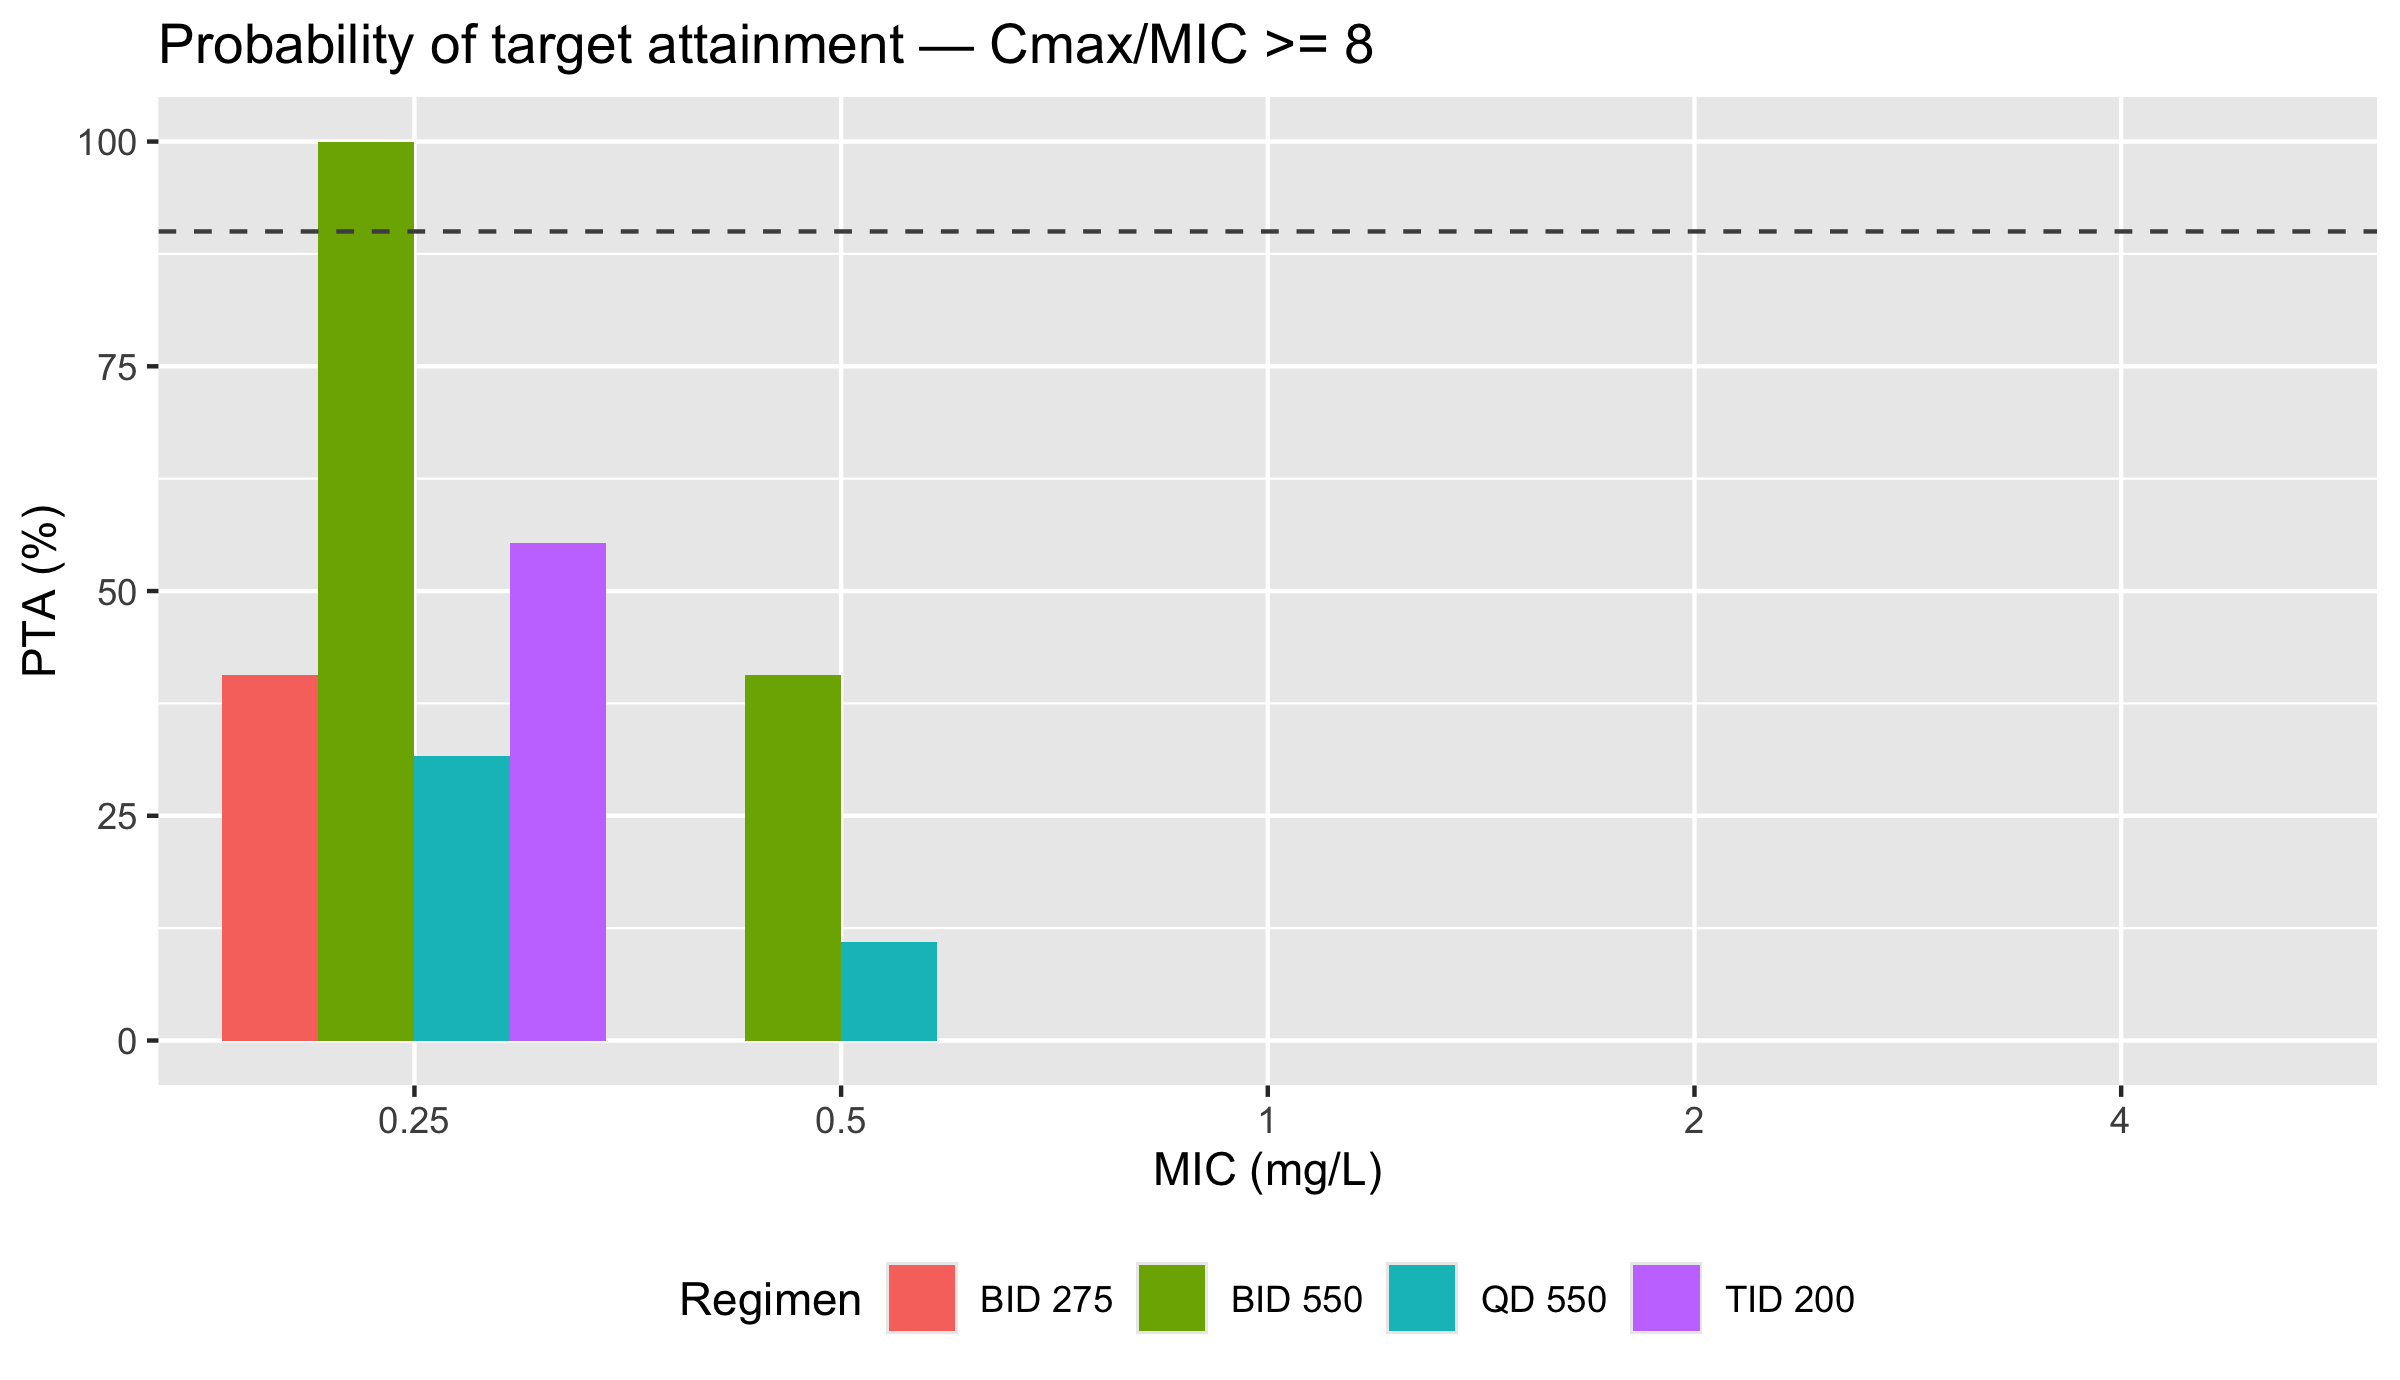
\includegraphics[width=0.8\textwidth]{s06_pta.png}
\caption{PTA of the peak target for the winner's fractionation options (also \cref{fig:res-ga-pta}).}
\label{fig:app-ga-pta}
\end{figure}

\begin{table}[htbp]
\centering
\caption{Convergence of the in-the-loop run (best-of-generation).}
\label{tab:app-ga-conv}
\begin{tabular}{rccc}
\toprule
Generation & best $F_{96}$ (\%) & best $\CMIC$ & median dose (mg) \\
\midrule
1 & 92.17 & 20.40 & 834 \\
5 & 95.53 & 27.00 & 993 \\
10 & 96.64 & 30.19 & 1000 \\
20 & 96.93 & 30.88 & 1000 \\
30 & 96.99 & 30.96 & 1000 \\
40 & 97.03 & 31.05 & 1000 \\
50 & 97.07 & 31.12 & 1000 \\
60 & 97.11 & 31.18 & 1000 \\
\bottomrule
\end{tabular}
\end{table}

\section{Converged front}
The converged front (generation 60 checkpoint; best $F$ within 0.1\% of final since generation 20) contains 3 near-identical non-dominated candidates at the component maxima --- the corner analyzed in \cref{sec:res-ga-convergence}. Rank-1 candidate: \textbf{TOBP-001} (999.8 mg, multiplier $\times$125.0, $F_{96} = 97.11\%$, $\CMIC = 31.18$, $\AMIC = 172.33$). The dose-scan analysis (\cref{tab:app-s07-dosescan}) provides the interior-region answer the corner cannot: the minimal peak-target-attaining dose is 250 mg once daily (Cmax$_{ss}$/MIC 8.0), and the 80--120 exposure band is attained from 467 mg.

% =====================================================================
% Appendix Q — Plausibility Audit: Benchmarks for the Enhancement Requirement
% =====================================================================
\chapter{Plausibility Audit: Benchmarks and Requirement Data}
\label{chap:app-audit}

\section{Literature benchmarks for permeability enhancement}
\begin{table}[htbp]
\centering
\caption{What the enhancement literature actually supports, versus what the targets require.}
\label{tab:app-benchmarks}
\small
\begin{tabular}{p{4.6cm}p{3.4cm}p{5.4cm}}
\toprule
Benchmark & Claimed/supported enhancement & Transfer to intestinal permeability \\
\midrule
HIP logP shift (tobramycin--docusate, in vitro) & 1500$\times$ \emph{partition coefficient} \citep{Asad2023} & Not a permeability multiplier; complex dissociates 20\% at intestinal pH \\
HIP in vivo (octreotide, pigs) & oral $F$ gain 3--5$\times$ \citep{Bonengel2018} & Closest in-vivo analogue for polycationic peptides \\
Oral SNAC platform (semaglutide) & $F \approx 1\%$ --- flagship success of oral PE platforms & Regulatory precedent; illustrates domain ceiling \\
Nominal combination platform (this thesis) & $\times$20 apparent $P_{int}$ & Aggressive; testable (Caco-2/Ussing of HIP complex) \\
Requirement for both targets @ 993 mg & $\geq\times$20 & S08 requirement map (\cref{chap:results-ga}) \\
Cited-bounds maximum (GA corner) & $\times$125 & Minimizes dose (467 mg attains the band floor); trough at the monitoring line \\
\bottomrule
\end{tabular}
\end{table}

\section{Numerical integrity notes}
\begin{enumerate}
\item \textbf{F clamped at 100\%.} The winner needs no clamp ($F_{96} = 97.11\%$); only the top S02 grid point overshoots numerically (100.41\% at $P_{int} = 10^{-6}$ dm/min) and is clamped there. All thesis statements enforce $F \leq 100\%$.
\item \textbf{Superposition inflation.} Steady-state AUC by superposition agrees with true seven-day dosing within $\approx$3\% (48.0 vs 49.6 mg·h/L at the $\times$20 probe; mass balance AUC$_{\tau}$ = $F \cdot$ dose/CL holds within 0.1\% at true steady state with CL 5.63 L/h). Screening sweeps legitimately use superposition; headline values use true dosing.
\item \textbf{Stale-run incident.} An earlier S07 run reported winner troughs of 4.2 mg/L; the cause was a silently failing dose override in the first script version (wrong application path). The corrected battery (32.2 / 172.3 / 1.21 on the final platform) agrees with the independent S08 path --- the incident is retained in the debugging journal (\cref{chap:app-debug}) as a lesson on silent override failures.
\end{enumerate}

\section{Requirement data}
The complete S08 requirement map (9 multipliers $\times$ 8 doses, 72 native runs) is committed at \texttt{results/studies/S08\_requirement\_map.csv}; the dose-scan per multiplier at \texttt{results/studies/S08\_dose\_scan\_<mult>.csv}. Headline rows appear in \cref{tab:res-reqmap}.

% =====================================================================
% Appendix R — Complete candidate evaluation data (S-battery)
% =====================================================================
\chapter{Candidate Evaluation: Battery Data}
\label{chap:app-battery}

Both candidate formulations were evaluated with the standard battery of \cref{sec:res-battery} (script \texttt{molecule\_battery.R} under \texttt{pksim/studies/}; outputs under \texttt{results/molecule\_A/} and \texttt{results/molecule\_B/}). This appendix collects the per-block tables that do not appear in the main text.

\section{Identity cards (cited component factors)}

\begin{table}[htbp]
\centering
\caption{Component factors at the candidate compositions (decoded via the shared enhancement model).}
\label{tab:app-identity}
\resizebox{0.96\textwidth}{!}{%
\begin{tabular}{lcccc}
\toprule
Component & TOB-161-A value & factor & TOBP-001 value & factor \\
\midrule
logP$'$ (HIP complex)        & +1.5  & 18.7$\times$ & +1.6 (measured cap) & 20.0$\times$ \\
SEDDS fraction (sum)         & 100\% & 1.00$\times$ & 160\% & 1.60$\times$ \\
Nanoparticle size            & 50 nm & 1.50$\times$ & 50 nm & 1.50$\times$ \\
C10 loading                  & 50\%  & 1.60$\times$ & 50\%  & 1.60$\times$ \\
Polymer loading              & 30\%  & 1.30$\times$ & 29.3\% & 1.29$\times$ \\
Chitosan coating             & on    & 1.15$\times$ & on    & 1.15$\times$ \\
Enteric coating              & on    & 1.10$\times$ & on    & 1.10$\times$ \\
\midrule
\textbf{Emergent multiplier} & \multicolumn{2}{c}{$\times$73.9} & \multicolumn{2}{c}{$\times$125.0} \\
\bottomrule
\end{tabular}}
\end{table}

\section{Dose proportionality}
Single-dose Cmax and AUC24 scale linearly with dose across 138--1100 mg (TOB-161-A) and 250--2000 mg (TOBP-001); deviation from proportionality $<$2\% at all tested doses (linear kinetics, no solubility limitation at these doses: 2000 mg $\approx$ 21 mL of the 94 mg/mL solution).

\section{PK/PD targets vs the MIC panel (steady state, QD)}

\begin{table}[htbp]
\centering
\caption{Steady-state target attainment vs MIC (true 7-day once-daily dosing).}
\label{tab:app-mic-panel}
\resizebox{\textwidth}{!}{%
\begin{tabular}{lcccc|cccc}
\toprule
 & \multicolumn{4}{c|}{TOB-161-A (550.6 mg)} & \multicolumn{4}{c}{TOBP-001 (1000 mg)} \\
MIC (mg/L) & Cmax/MIC & AUC$_{\tau}$/MIC & Cmin (mg/L) & fT$>$MIC & Cmax/MIC & AUC$_{\tau}$/MIC & Cmin (mg/L) & fT$>$MIC \\
\midrule
0.25 & 54.3 & 349  & 4.21 & 99.6\% & 129.2 & 690  & 4.81 & 99.6\% \\
0.5  & 27.2 & 175  & 2.11 & 99.6\% & 64.6  & 345  & 2.41 & 99.6\% \\
1    & 13.6 & 87.3 & 1.05 & 99.6\% & 32.3  & 172  & 1.20 & 99.6\% \\
2    & 6.8  & 43.6 & 0.53 & 78.4\% & 16.1  & 86.2 & 0.60 & 99.6\% \\
4    & 3.4  & 21.8 & 0.26 & 42.9\% & 8.1   & 43.1 & 0.30 & 87.6\% \\
8    & 1.7  & 10.9 & 0.13 & 20.5\% & 4.0   & 21.6 & 0.15 & 61.4\% \\
\bottomrule
\end{tabular}}
\end{table}

\section{Uncertainty propagation (S09)}

\begin{table}[htbp]
\centering
\caption{Component-uncertainty propagation (20\,000 draws, graded lognormal sigmas; S09).}
\label{tab:app-s09}
\small
\begin{tabular}{lcc}
\toprule
 & TOB-161-A & TOBP-001 \\
\midrule
Multiplier (point [CI95])   & 73.9 [12.5--431] & 125.0 [21.1--730] \\
$F_{96}$ (\%) [CI95]        & 88.0 [35.3--100] & 96.2 [50.6--100] \\
AUC$_{ss}$/MIC [CI95]       & 87 [39--99]      & 172 [97--179] \\
PTA Cmax/MIC $\geq$8        & 81\%             & 99\% \\
PTA AUC$_{ss}$/MIC in 80--120 & 65\%           & 99\% \\
\bottomrule
\end{tabular}
\end{table}

\section{Methodological notes}
\begin{enumerate}
\item \textbf{True repeated dosing} is implemented by replicating the application event group in the PKML (one \texttt{Application\_k} per dose, exactly as PK-Sim itself represents multiple dosing; \texttt{make\_repeated\_pkml.py}), then setting the per-application dose and the calibrated permeability at simulation level.
\item \textbf{Mass balance check}: at steady state AUC$_{\tau}$ = $F \cdot$ dose/CL. TOB-161-A: 87.25 vs 87.38 mg$\cdot$h/L predicted (0.15\%); TOBP-001: 172.28 vs 172.20 (0.05\%).
\item \textbf{Superposition cross-check}: the screening-study superposition agrees with true dosing within $\approx$3\% (48.0 vs 49.6 mg$\cdot$h/L at the probe point), validating its use in the fast sweeps.
\item \textbf{Component OAT degeneracy}: under a purely multiplicative enhancement model, $\pm$20\% on any single factor shifts the multiplier identically --- the differentiated risk lives in the per-component sigmas (S09), not in the OAT ranges. Both are reported for transparency.
\item \textbf{Renal impairment}: $F$ is not identifiable when clearance changes (the oral AUC scales with CL); the B7 block therefore reports AUC, not $F$.
\end{enumerate}


\backmatter
\bibliographystyle{unsrtnat}
\bibliography{references}

\end{document}
